%%%%%%%%%%%%%%%%%%%%%%%%%%%%%%%%%%%%%%%%%%%%%%%%%%%%%%%%%%%%%%%%%%%%%%%%%%%%%%%%
% data_set.tex:
%%%%%%%%%%%%%%%%%%%%%%%%%%%%%%%%%%%%%%%%%%%%%%%%%%%%%%%%%%%%%%%%%%%%%%%%%%%%%%%%
\chapter{Search Analysis for Long-Lived Neutral Particles }
\section{Analysis Strategy}\label{Analysis}
The search for a Long-Lived Neutral Particle in final state with at least one late photon and large Missing Transverse Energy~(\MET) is described. The photon arrival time is measured using the Electromagnetic Calorimeter~(ECAL). We use a counting method to perform the search where an excess number of events with photon time above a timing threshold over the expected number of background events indicates the presence of a new physics phenomenon like the decay of the lightest neutralino into a late photon and a gravitino. Since a final state with at least a late photon and large \MET is difficult for standard model interactions to mimic, we expect most of the background events to arise from processes other than proton-proton~($pp$) collision events.
%%%%%%%%%%%%%%%%%%%%%%%%%%%%%%%%%%%%%%%%%%%%%
\subsection{Signal and Background Events}
The decay of the lightest neutralino~(\PSneutralinoOne) to a late photon~(\Pphoton) and gravitino~($\tilde{G}$), $\PSneutralinoOne\rightarrow\Pphoton + \tilde{G}$, gives rise to events whose final state consist of a late photon and large \MET due to the undetected gravitino~($\tilde{G}~$) and since the \PSneutralinoOne is produced from the cascade decay of heavier sypersymmetric particles like gluino~($\PSgluino$) or squark~($\Psquark$), \ie $\Pg\Pg\rightarrow \PSgluino\PSgluino \rightarrow \Pquark\APquark\Pquark\APquark\PSneutralinoOne\PSneutralinoOne$ or $\Pquark\APquark\rightarrow \Psquark\APsquark\rightarrow \APquark\Pquark\PSneutralinoOne\PSneutralinoOne$, we expect the final state of a signal event to include multiple hiph-\pt jets. Thus, the final state of a typical signal event comprises of at least one late high-\pt photon, large \MET and multiple high-\pt jets. The multiple high-\pt jets provides an additional handle during event selection to help suppress background events with no jets.
\par 
If at all there are any background events with a similar final state to the signal event, they must be atypical events with late photons, large \MET and jets in the final state produced from either $pp$ collisions or some other source(s) which we refer to as \textit{non-collision} .
\newline
These non-collision background events include the so-called proton \textit{Beam Induced Backgrounds} or beam halo, cosmic rays and spikes. 
\newline
The background events produced from $pp$ collisions~(collision background events) that can emulate signal events are those events for which the photon time and/or \MET are mis-measured or those events produced from satellite bunch crossings described in section \ref{Ghost} which have late photons in the final state. Other collision events that could have real \MET and a misidentified photon in the final state include: inclusive $\PZ +$jets/$\PW +$jets events, inclusive top-anti-top~($t\bar{t}) +$jets events and inclusive $\PZ\PZ$/$\PW\PW$/$\PW\PZ +$jets events which have true \MET through the $\PZ \rightarrow \Pnu\APnu$ and $\PW\rightarrow\Pe\APnue$ decays with the undetected neutrino~(\Pnu) giving rise to \MET. Multijets and QCD events on the other hand give rise to fake \MET~(instrumental \MET), where an undetected particle is not part of the event but the \MET arises due to poor reconstruction of the energies of the particles. The late photon arises when one of the jets or an electron is misidentified as a photon and its ECAL time is mis-measured. The other jets in the event might satisfy the high-\pt multiple jets requirement.
\subsection{Samples}
\subsection*{Datasets}
The data sample used for this search was recorded by the CMS detector and is equivalent to a total integrated luminosity of 19.1~\fbinv. It contains events passing an HLT trigger which requires that at least one photon belongs to the final state. These events were produced during LHC Run 1 $pp$ collisions at the center of mass energy, $\sqrt{S} = 8$\TeV.
\subsection*{Monte Carlo Samples}
The MC samples are made with \textit{Summer 2012} prescription of the calibration and alignment status of the CMS detector and pile up conditions at 8\TeV.
\newline
The SPS8 benchmark GMSB samples are produced for different mean lifetime~($c\tau$) of the lightest neutralino~(\PSneutralinoOne) ranging from 500\mm~($\tau = 1.7\ns$) to 10000\mm~($\tau = 33.3\ns$) for each effective SUSY breaking scale~($\mathbf{\Lambda}$) or mass of the lightest neutralino~($m_{\PSneutralinoOne}$) point. We vary $\mathbf{\Lambda}$ from 100\TeV to 220\TeV which is equivalent to $m_{\PSneutralinoOne}$ ranging from 139\GeVcc to 314\GeVcc.
Each sample has 50,000 events for each $c\tau$ and $\mathbf{\Lambda}$.  Table \ref{tab:mc_GMSB_sample} shows a summary of our signal MC samples used where for each sample, equally given is the number of events, cross-section and branching ratio for \PSneutralinoOne production and decay to $\gamma$ and $\tilde{G}$ for each $\mathbf{\Lambda}$.
\newline
The $\gamma +$jet MC samples were generated for different momentum of the colliding parton~($\hat{\pt}$) and normalized to the 19.1 \fbinv of integrated luminosity. The cross-sections, momentum of the colliding parton and the number of events in each sample is summarized in Table \ref{tab:mc_QCD_sample}. The $\hat{\pt}$ range is from 50\GeVc to 800\GeVc.

\vspace{5mm}
%\paragraph*{}\mbox{}\\
\begin{minipage}{0.94\textwidth} 
\begin{center}
%\begin{table}[ht]
%\renewcommand\arraystretch{1.2}
\centering
\begin{tabular}{c c c c c c}
     %\hline
       %\textbf{Signal MC [mGMSB~(SPS8)]}
       \toprule
        \hline
        $\Lambda$~[TeV] & $m_{\PSneutralinoOne}$[\GeVcc] & $c\tau$~(mm) & $\sigma_{LO}$~(pb) & \bfseries{Total Events} & \bfseries{BR}\\
       \hline
       \toprule
       100 & 140 &500-10,000  & 0.368  & 50,000 & 0.9444\\
       120 & 169 &500-10,000  & 0.133  & 50,000 & 0.9042\\
       140 & 198 &500-10,000  & 0.0574 & 50,000 & 0.8711\\
       160 & 227 &500-10,000  & 0.0277 & 50,000 & 0.8464\\
       180 & 256 &500-10,000  & 0.0145 & 50,000 & 0.8282\\
       220 & 314 &500-10,000  & 0.0044 & 50,000 & 0.8282\\
      % 260 & 250-12,000  & 0.0015 & 50,000 & 0.8282\\
      % 300 & 500-12,000  & 0.0008 & 50,000 & 0.8282\\
       \hline
       \bottomrule
       \end{tabular}  
\captionof{table}{Signal GMSB SPS8 Monte Carlo samples for different $\mathbf{\Lambda}$ with $50\cm < c\tau < 1000\cm$ and Branching Ratios~(BR).}
\label{tab:mc_GMSB_sample}
%\end{table}
\end{center}
\end{minipage}

\vspace{5mm}
%\paragraph*{}\mbox{}\\
\begin{minipage}{0.90\linewidth} 
\begin{center}
%\begin{table}[ht]
%\renewcommand\arraystretch{1.2}
\begin{tabular}{c c c}
\toprule
\hline
$\hat{\pt}$ & $\sigma_{LO}$ (pb) & \bfseries{Number of Events}\\
\hline
\toprule
 50 $\sim$ 80  & 3322.3  & 1995062 \\
 80 $\sim$ 120 &  558.3  & 1992627 \\
120 $\sim$ 170 &  108.0  & 2000043 \\
170 $\sim$ 300 &   30.1  & 2000069 \\
300 $\sim$ 470 &    2.1  & 2000130 \\
470 $\sim$ 800 &  0.212  & 1975231 \\
\hline
\bottomrule
\end{tabular}
\captionof{table}{The $\gamma +$ jets samples for $\hat{\pt}$ from  50\GeVc to 800\GeVc }
\label{tab:mc_QCD_sample}
%\end{table}
\end{center}
\end{minipage}

\vspace{5mm} 
%%%%%%%%%%%%%%%%%%%%%%%%%%%%%%
\section{ECAL Timing}
In this section we describe the measurement of the photon time, tuning of the time from MC and the observation of late photons from satellite proton bunch collisions.

\subsection{Photon Time Measurement for this Analysis}
The electromagnetic shower of a photon spreads across several crystals and so the photon's time can be measured using the time from one or all these crystals. For example, the photon's arrival time can come from either the reconstructed time~($ t_{reco}$) of the \textit{seed crystal}~(crystal with the highest energy deposit), $t_{seed}$, or a weighted average time calculated using the reconstructed time and uncertainty of each crystal of the photon's supercluster:
\begin{equation}{\label{eq:AVETIME}}
t_{Ave} = \frac{\sum_{i=1}^N\frac{t^{i}_{reco}}{\sigma_{i}^{2}}}{\sum_{i=1}^{N}\frac{1}{\sigma_{i}^{2}}},
\end{equation}
where $N$ is the total number of crystals of the supercluster, $t^{i}_{reco}$  and $\sigma_{i}$ are the time and uncertainty on the reconstructed time of each crystal, respectively. 
Figure \ref{fig:TIME} shows a comparison of the seed time, $t_{seed}$, and the average time, $t_{Ave}$, as the photon's time. Both distributions are normalized to total number of events.

\vspace{5mm}
\begin{minipage}{0.90\linewidth} 
\begin{center}
\mbox{
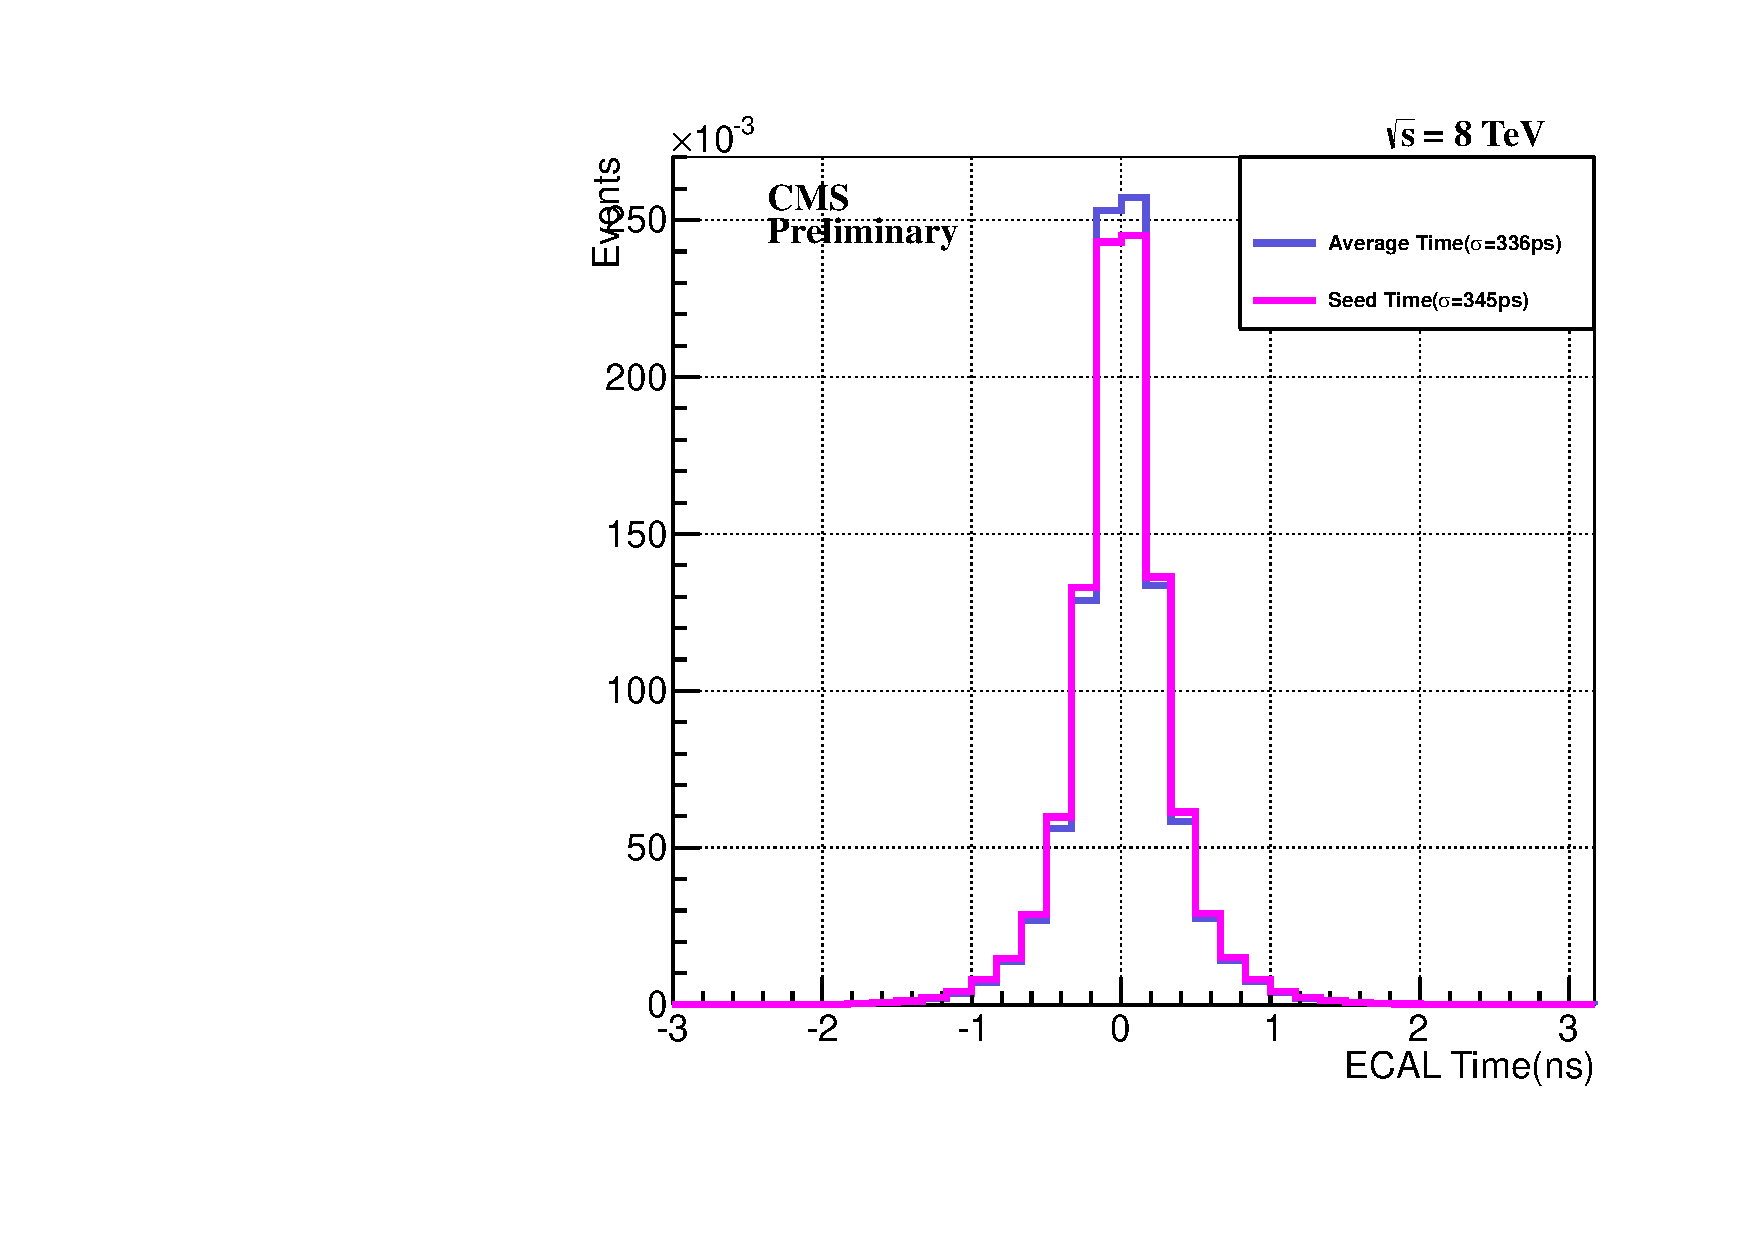
\includegraphics[height=0.60\textwidth, width=0.7\textwidth]{THESISPLOTS/ECAL-SeedVsAveTime-Zee.pdf}
%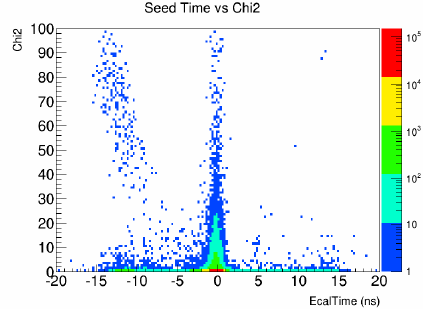
\includegraphics[height=6cm, width=0.5\textwidth]{THESISPLOTS/Seed-Time-Chi2.png}
}
\captionof{figure}{Seed~(black) and Average~(blue) times as the measured photon time.}
\label{fig:TIME}
\end{center}
\end{minipage}

\vspace{5mm}
The width~($\sigma$) of both Gaussian distributions are similar, the standard deviation for the seed time, $\sigma_{t_{seed}} = 345$\ps, and that for the average time, $\sigma_{t_{Ave}} = 336$\ps. We expected the standard deviation of the average time to be smaller than the seed time, however due to the presence of crystals with atypically large times as seen in the tails of the average time distribution the average time shows no improvement on the seed time. The average time is susceptible to spurious timing measurements. If one of the crystals in the supercluster happens to be poorly time calibrated or embedded with a spike, the photon time will be biased and this happens often for $t_{Ave}$ although the magnitude of the bias is smaller.
 \newline
We use the seed time as the photon's time in this analysis, however, the presence of anomalous signals from spikes, noisy crystals and pile-up events demand a robust method for checking that the photon time has been properly reconstructed since we use the photon's time as our main observable for distinguishing background from signal events. To perform this check we use the $\chi^{2}$ of the photon's time computed using the average time and reject those photons with very large $\chi^{2}$ which is often the case for photons with spurious timing measurements. The $\chi^{2}$  is computed as
\begin{equation}\label{eq:CHI2}
\chi^{2} = \sum^{N}_{i=0}\frac{(t^{i}_{reco} - t_{Ave})^{2}}{\sigma_{i}^{2}}
\end{equation}
where $N$ is the number of crystals in the photon supercluster, $t^{i}_{reco}$ and $\sigma_{i}$ are the time and uncertainty from each crystal, and $t_{Ave}$ is the average time defined in Equation \ref{eq:AVETIME}. The $\chi^{2}$ is used to help distinguish non-isolated spikes from true photons and a distribution of the normalized $\chi^{2}$ against the photon time in Figure \ref{fig:Chi2} show that spikes which have been misidentified as photons have large $\chi^{2}$ and large negative time.
 
 \vspace{5mm}
%\paragraph*{}\mbox{}\\ 
\begin{minipage}{0.90\linewidth} 
\begin{center}
\mbox{
%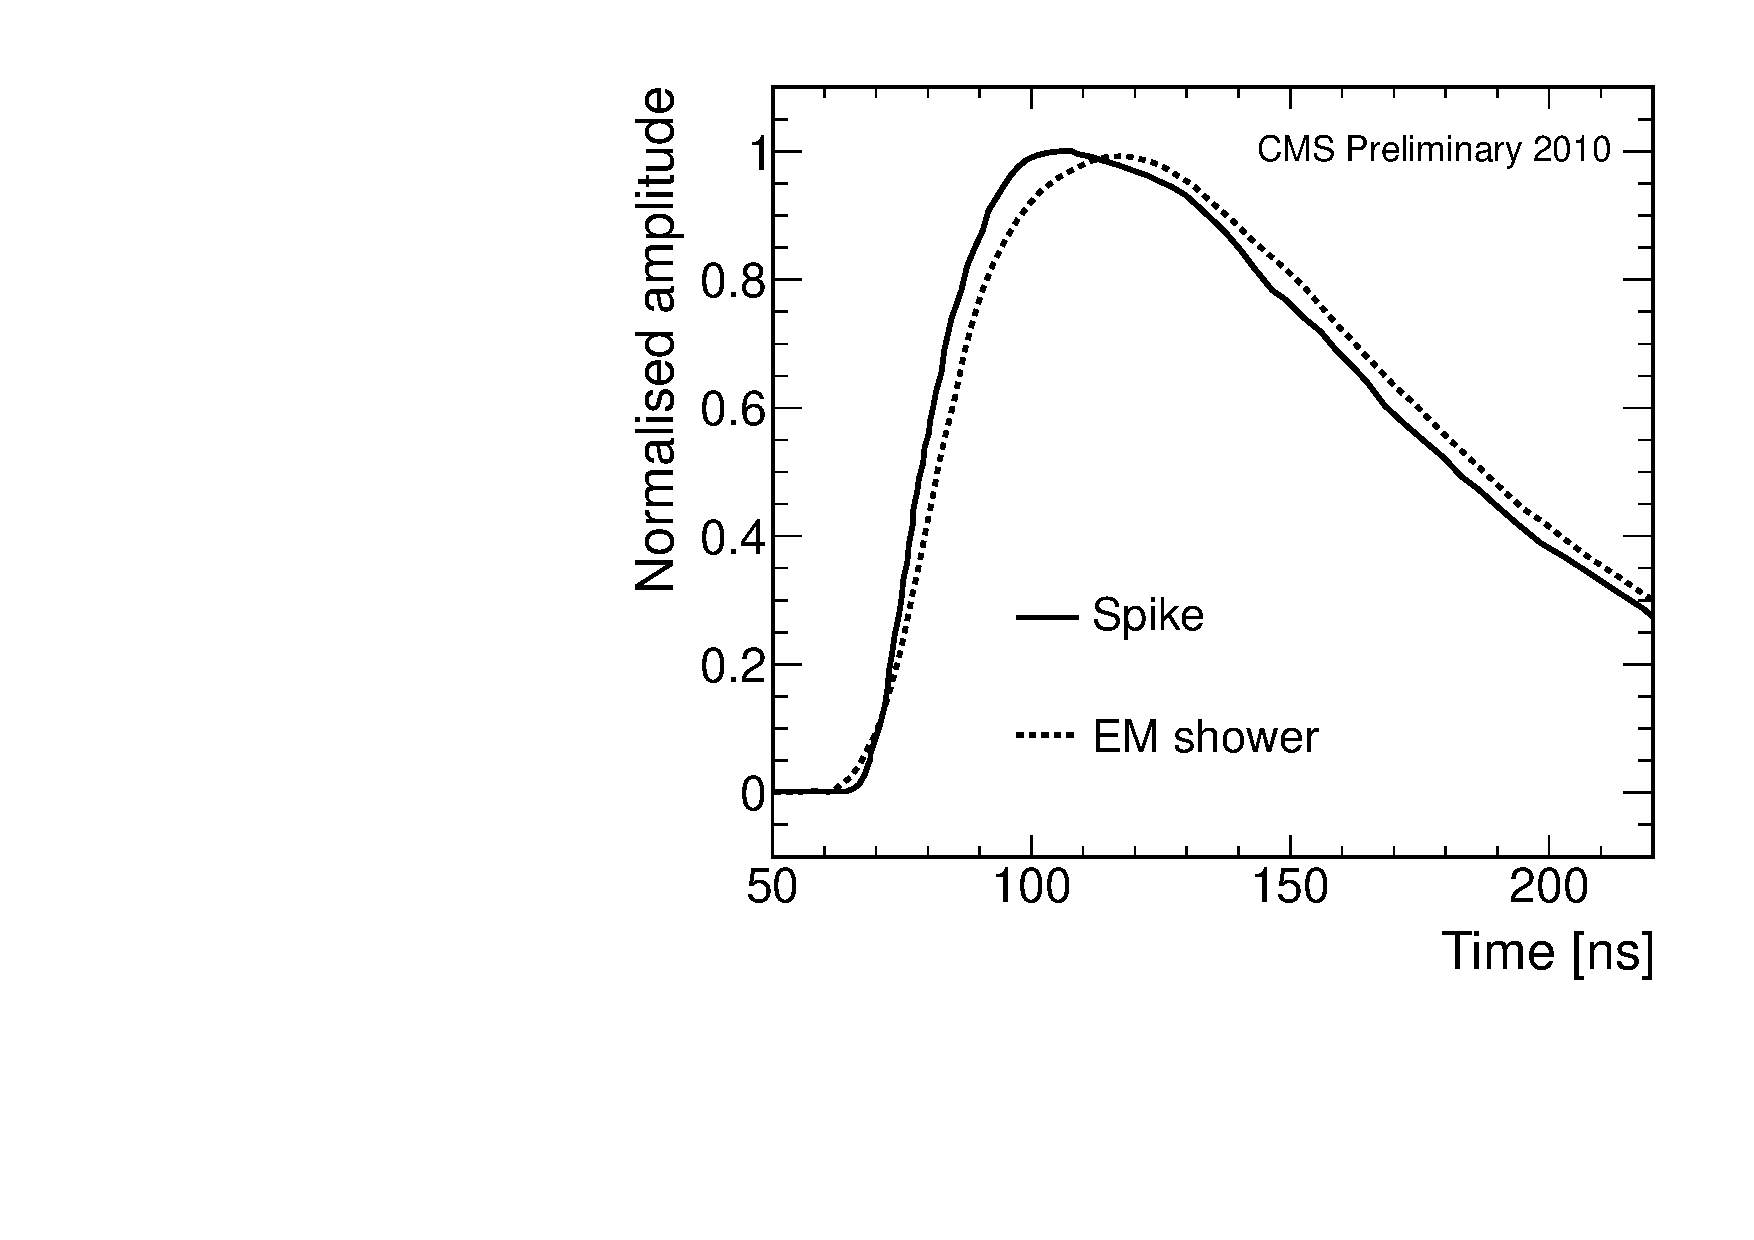
\includegraphics[height=.450\textwidth, width=0.45\textwidth]{THESISPLOTS/spike_pulse_shape.pdf}
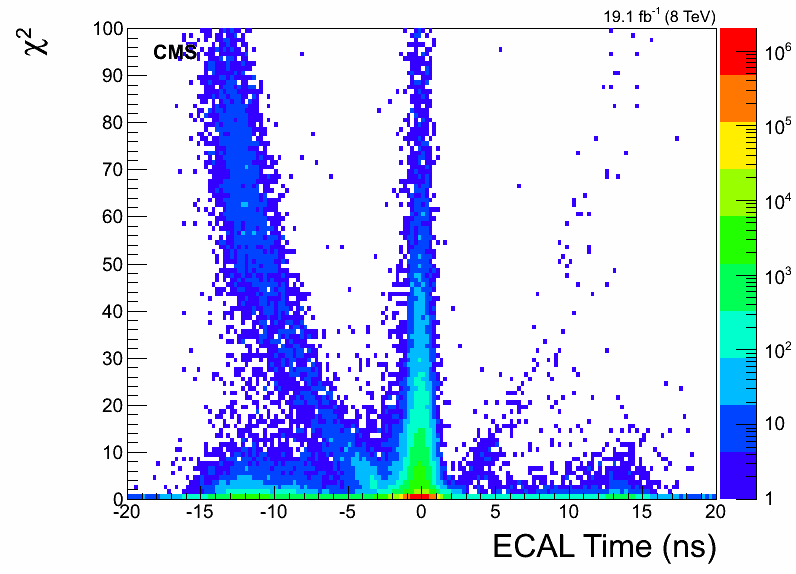
\includegraphics[height=.450\textwidth, width=0.65\textwidth]{THESISPLOTS/seedTime_Chi2.png} }
\captionof{figure}{A $\chi^{2}$ against photon time distribution. Spikes misidentified as photons have very large $\chi^{2}$ and negative time particularly the region where $\chi^{2} > 4$ and $t < -4\ns$.}
\label{fig:Chi2}
\end{center}
\end{minipage}

\vspace{5mm}
It is clear from Figure \ref{fig:Chi2} that most of the true photons have time around zero but there are also photons with time, $t\approx 0$, with large $\chi^{2}$. The contributions from these photons with spurious time measurements especially those with large negative times which we call spikes can be reduced by rejecting photons with $\chi^{2} > 4$. 
%%%
%%%%
\subsubsection{Timing from Monte Carlo}
It is challenging to properly simulate the time of MC events so that it captures the conditions of the ECAL sub-detector during data recording. As a result, the mean time and root mean squared~(RMS) from MC events does not agree perfectly with those in data.
We correct for this disagreement by shifting the mean time and smearing the RMS with an additional Gaussian convolution on the photon time of MC events so that the MC mean time and RMS matches that of data.
The amount~(the difference between data and MC photon times) of shifting and smearing required is obtained using selected 1 or 2 jets events and to ensure that true photon events are used, we select events whose final state consist of 1 or 2 jets with in-time photons~($|t_{\gamma}| < 2\ns$) of photon $\pt > 80$\GeV from data and $\gamma +$jets MC samples. Shown in Figure \ref{fig:DATAMCTime} is the in-time photon time distributions for data and $\gamma +$jets  MC samples before~(left plot) and after~(right plot) the corrections are applied on the photon time of $\gamma +$jets  MC events. We see good agreement between MC and data photon time.

\vspace{5mm}
%\paragraph*{}\mbox{}\\
\begin{minipage}{0.90\linewidth} 
\begin{center}
\centering
\mbox{
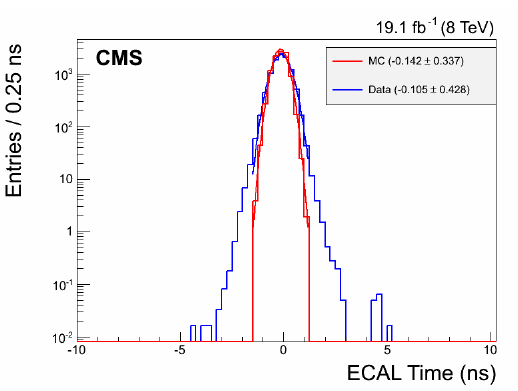
\includegraphics[height=0.6\textwidth, width=0.5\textwidth]{THESISPLOTS/MC_Vs_DataTimeB4Calib.png}
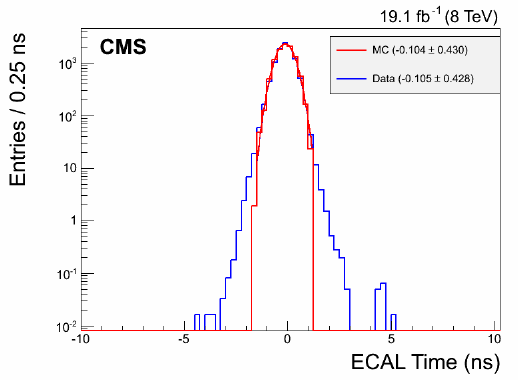
\includegraphics[height=0.6\textwidth, width=0.5\textwidth]{THESISPLOTS/MC_Vs_DataTimeAferCalib.png}
}
\captionof{figure}{Time distributions of in-time photons from  $\gamma +$ jets MC~(blue) and data~(red) samples before~(left) and after~(right) we adjusted the MC photon time.}
\label{fig:DATAMCTime}
\end{center}
\end{minipage} 
%We performed the same smearing for all MC samples used in our analysis.
%\newline
% It is worth noting that the difference of 125~ps between $t^{MC}_{reco}$ and $t^{DATA}_{reco}$ compared to 500~ps ECAL timing resolution is not enough to enormously impact our event selection. %however, simulating photons ECAL time in the tails of the time distribution still remains.
%%%% A possible solution for this is to select only properly time calibrated crystals of the supercluster for computing the average time or simply used the times from crystals of the \textit{seed basic cluster}. A supercluster is said to consist of many smaller clusters called \textit{basic clusters}, and the average time of the cluster with the highest energy~(seed basic cluster) can also be used as the particle's measured arrival time.
%%time which equally have large normalized $\chi^{2}$ values. We expect large $\chi^{2}$ values in cases where the time measurements from non-seeded crystals is inconsistent with the time measurement from the seed crystal. We also observe that,  can reduce with 99.2\% efficiency, photon contributions from spikes~(where a neutron, embedded in a jet, hits directly the photo-detectors and produces a spike) and photons with mis-measured ECAL time.
%%%%%%%%%%%%%%%%%%%%%%%%%%%%%%%%%%%%%%%%%%%%%%%%%%%%%%%%%%%%%%%%%%%%%%%%%%%%%%%%%%%%%%
\subsection{Satellite Bunches}
Satellite proton bunches which lead or trail the  LHC main proton bunch with a time spacing of 2.5\ns  are also a source of background with positive times from Beam halo-induced photons observed in ECAL. Figure \ref{fig:TIMEECAL} shows the photon time for photons with $\pt > 50$\GeVc in ECAL. The 2.5\ns discrete pattern in the photon time confirm the presence of satellite beam halo-induce photons in the endcap~($1.47 < \eta < 3.0$)~(mostly) and barrel~($|\eta| < 1.47$) regions. We find that proton Beam halo-induced photons is a major background to late photons. 

\vspace{5mm}
\begin{minipage}{0.90\linewidth} 
\begin{center}
\centering
\mbox{
%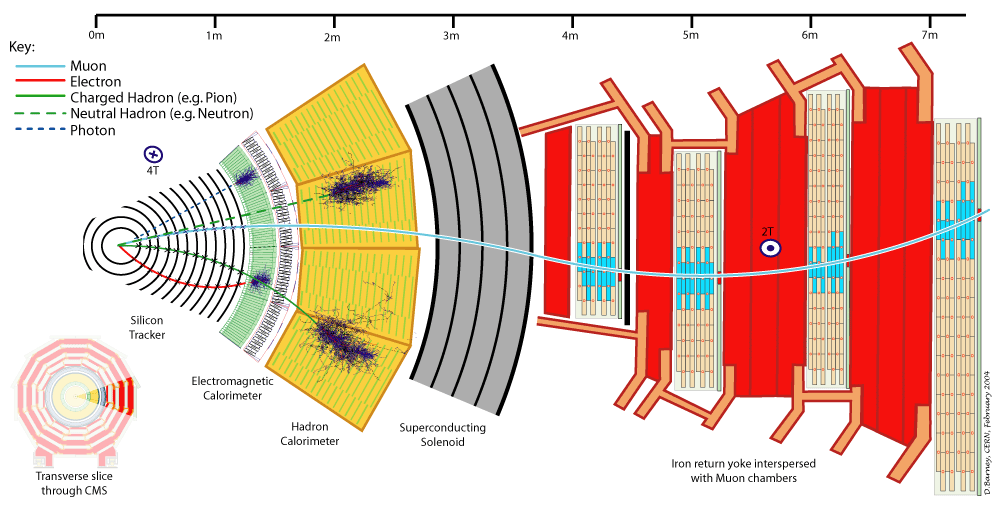
\includegraphics[scale=0.2]{THESISPLOTS/CMS_Slice.png}
%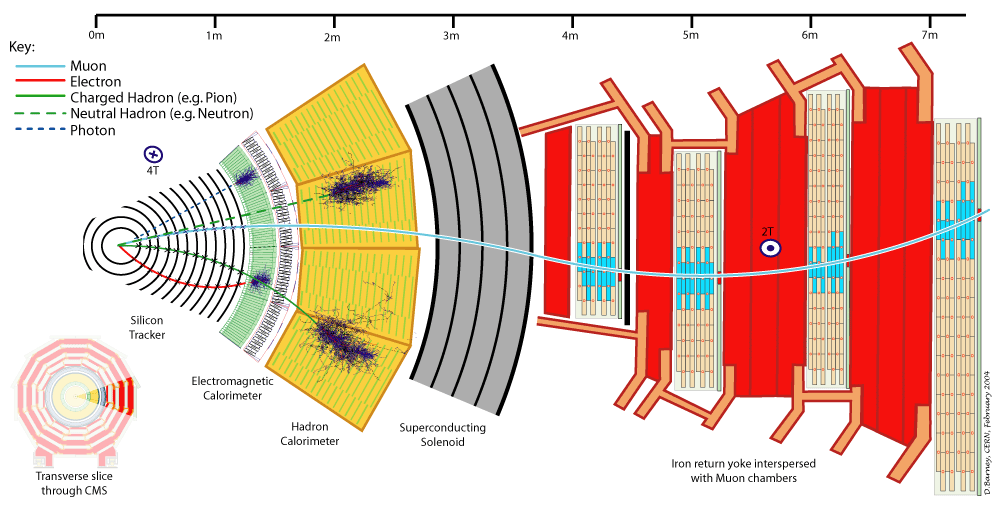
\includegraphics[scale=0.2]{THESISPLOTS/CMS_Slice.png}
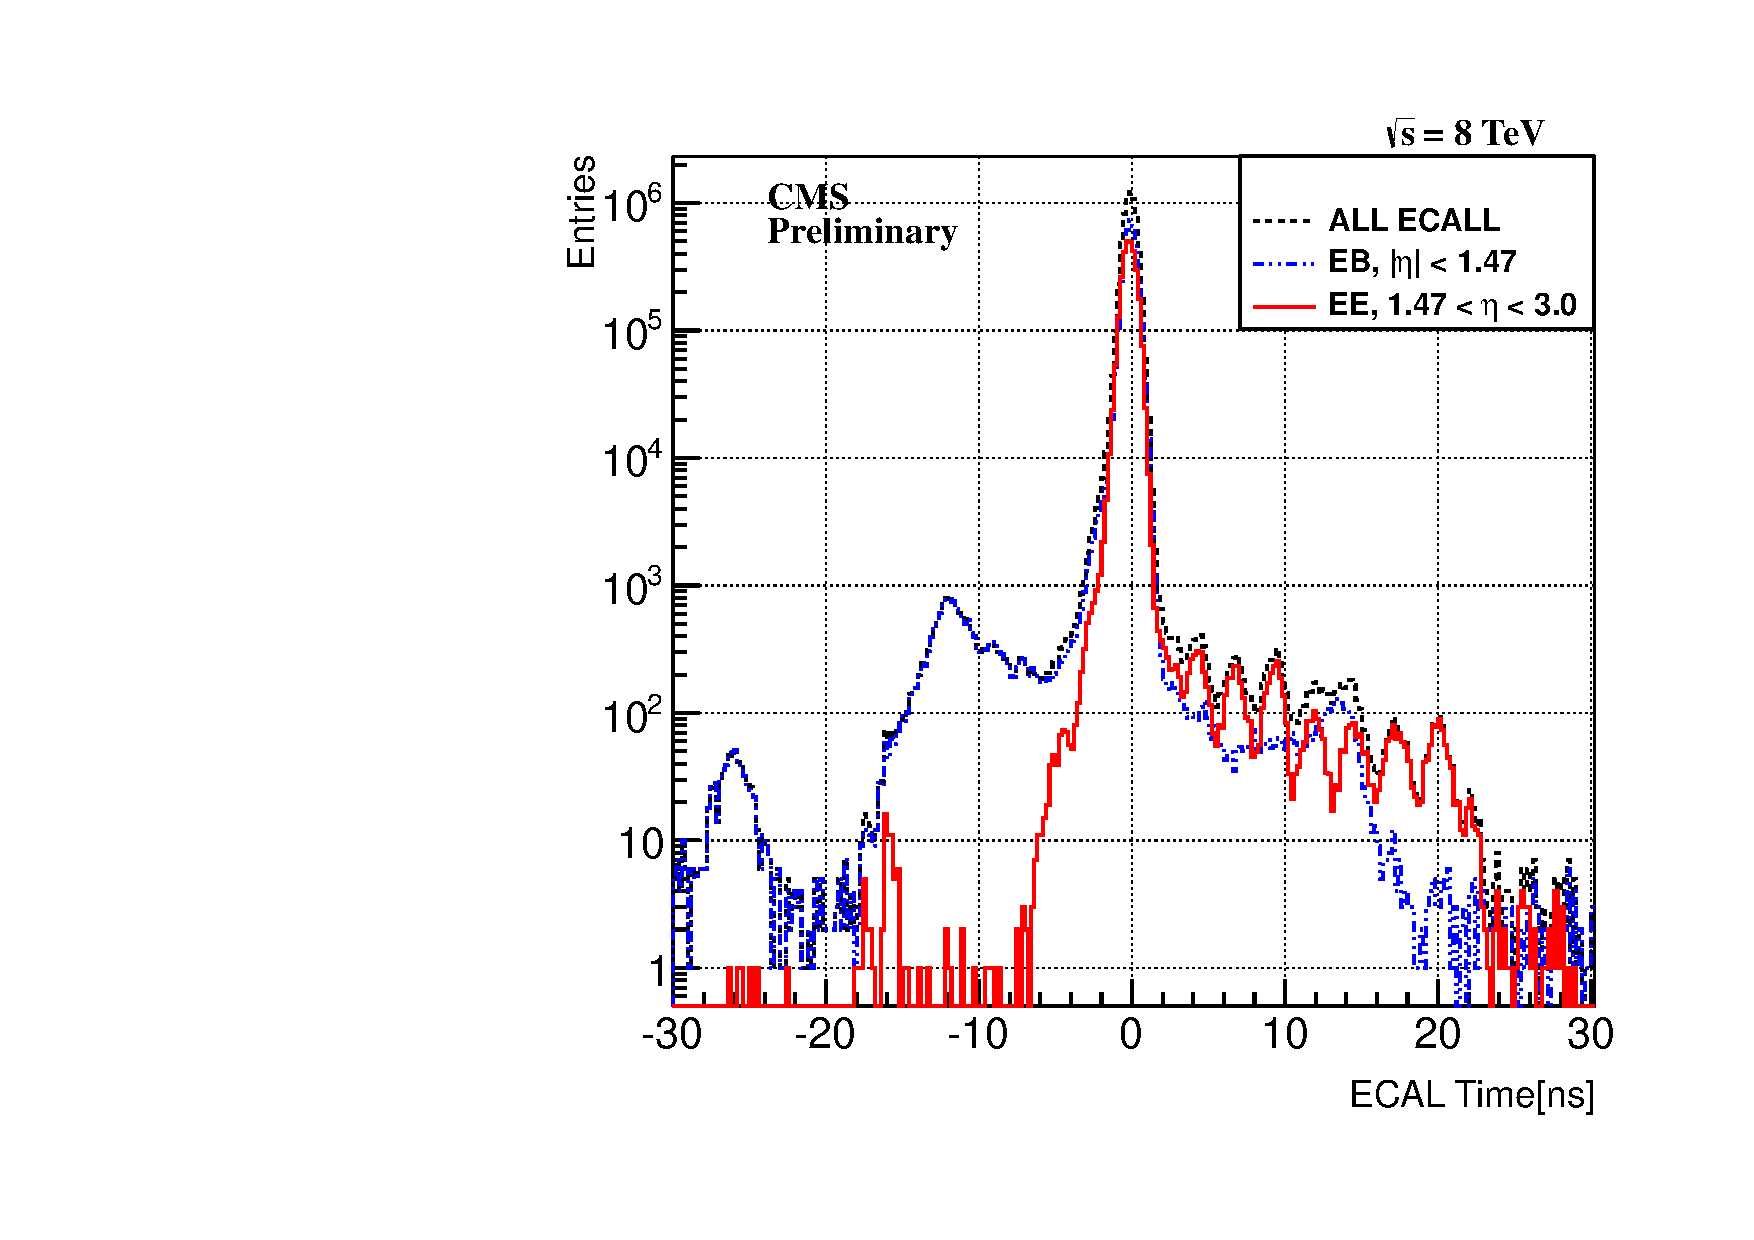
\includegraphics[height=0.60\textwidth, width=0.85\textwidth]{THESISPLOTS/PhotonTimeALLVsEBVsEE.pdf}
}
\captionof{figure}{Time distribution of photons in barrel~(\textcolor{blue}{EB}), endcap~(\textcolor{red}{EE}) and all of ECAL~(\textcolor{black}{ALL ECAL}) with $\pt > 50\GeV$ from data. A $2.5$\ns delay timing pattern is observed in ECAL with clarity in EE.}
\label{fig:TIMEECAL}
\end{center}
\end{minipage}

 %These out-of-time photons are produced  from beam halo muons from protons in \textit{Ghost}/\textit{Satellite} bunches or RF cavity, described in section \ref{Ghost}. We consider these events as background to our delayed photon signal. In addition to developing methods to tag and veto these events, a simple estimate of their contribution can be made using the ratio of the number of protons in the ghost RF cavities or bunches to the main proton bunches taken from the proton population in the RF cavity of the LHC proton filling profile. From this ratio, we estimate that one in every $100,000$ photons observed in ECAL particularly the endcaps, is from beam halo muons produced by ghosts bunches. Their presence is not clearly visible in the barrel as in the endcaps as they will be highly smeared in the barrel because their time is dependent on $\eta$ which is not the case in the endcaps. 
%is because very few of these photons are produced with high enough transverse momentum, \pt, to travel to the barrel and survive the 50\GeVc requirement. 
%\newline
%Our observation of this phenomenon together with the sub-par ECAL time resolution in the endcaps compared to the barrel, means, this analysis only uses photons belonging to the barrel.
%\newline

%%%
\subsection{\MET Adjustments}
In the formation of energy clusters which are used for event reconstruction by the particle flow~(PF) algorithm "out-of-time" energy deposits in ECAL are excluded. The reason is because the PF algorithm avoids energy deposits from particles like cosmic muons and machine-induced backgrounds which are not produced from the main $pp$ bunch collisions, as these are often out-of-time. Because of the exclusion, the out-of-time photon's transverse energy, \et, is not included in the calculation of missing transverse energy or \ETslash\hspace{0.15cm}~(from now on we will be using for convenience \ETslash\hspace{0.15cm} instead of \MET as the symbol for missing transverse energy) of the event. This exclusion introduces differences in the calculation of \ETslash\hspace{0.15cm} for in-time~($|t_{\gamma}| < 3.0$~ns) and for out-of-time photon events. 
\newline
Since we are searching for events with late arrival time photons coming from $pp$ collisions, we correct the particle flow reconstructed \ETslash\hspace{0.15cm}~(PF-MET) for events with out-of-time photons  by subtracting the out-of-time photon's $\ET$ from \ETslash\hspace{0.15cm}  and introduce an additional missing transverse energy variable defined as ${\ETslash}^{\gamma}\hspace{0.15cm} = \ETslash\hspace{0.25cm} - \et^{\Pphoton} $, in our final event selection. 
%%The difference between $\ETslash$\hspace{0.25cm} and ${\ETslash}^{\gamma}$ is given as
%%\begin{enumerate}
%%\item ${\ETslash}$~ : PF-MET equal to $\ETslash$\hspace{0.25cm} from standard event reconstruction.
%%\item ${\ETslash}^{\gamma}$~: PF-MET with photon \ET vector subtracted \ie ${\ETslash}^{\gamma} = \ETslash\quad - ~\et$ of the  out-of-time photon.
%% \end{enumerate}
%The distributions for ${\MET}_{1}$ and ${\MET}_{2}$  against ECAL time can be seen in figure \ref{fig:METS}.
%\begin{center}
%\centering
%\mbox{
%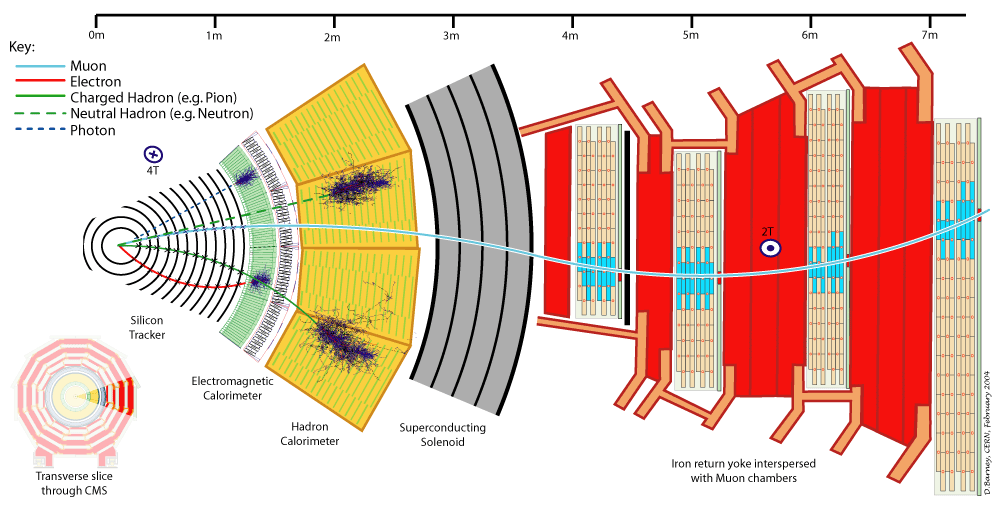
\includegraphics[scale=0.2]{THESISPLOTS/CMS_Slice.png}
%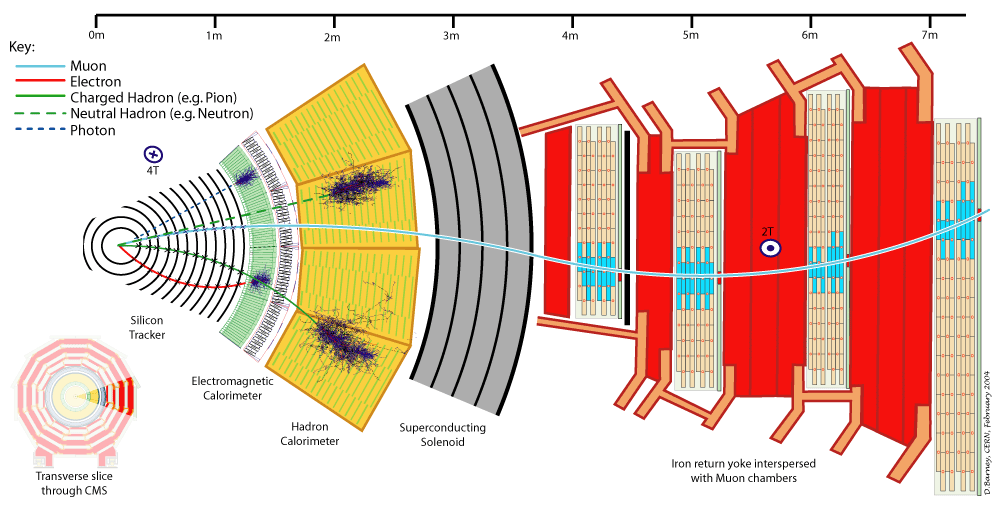
\includegraphics[scale=0.2]{THESISPLOTS/CMS_Slice.png}
%\captionof{figure}{Figure showing \MET distributions for events with out-of-time and in-time photons. ${\MET}_{1}$ and ${\MET}_{2}$ definitions are given in context. }
%\label{fig:METS}
%\end{center}
\section{Event Selection}
Our event selection happens in two stages. The first stage is a L1 trigger at online and a higher level trigger~(HLT) which is a software implementation of multiple selection modules designed to be efficient at selecting events with a delayed photon in the final state. The L1 trigger selects energy deposits in ECAL above a certain noise threshold while the HLT selects events with at least one triggered photon. The second stage happens offline where our signal-like event selection requirements are applied. 
\newline
The offline event selection criteria is designed to select signal-like events whose final state have at least a single photon, multiple jets and large \ETslash\hspace{0.15cm}. The multiple jets arise from the cascade decay of gluino or squark to other quarks or gluons, in addition to the lightest neutralino. We require multiple jets in the event selection to suppress non-collision background events like cosmic and beam halo muons which are inherently not associated with jets.
%and $pp$ collision background events like the ElectroWeak~(EWK) background events of $\PW \rightarrow e + \nu$ and $t\bar{t}$ decays, where the top~($t$) decays to a $b$ quark and a \PW boson 100\% of the time. These events with \PW boson can produce fake photons~(misidentified electron as photon) and real \ETslash\hspace{0.15cm} arising from the presence of the neutrino~($\nu$). 
\newline 
Collision background events with multiple jets where one of the jets is misidentified as a photon are equally suppressed by requiring the jet to be purely hadronic \ie the jet must have a greater hadronic energy fraction to electromagnetic energy fraction. 
\newline
We only select events whose late photon(s) is in the barrel~($|\eta_{\gamma}| < 1.479$) and the photon has a high transverse momentum. The high photon's transverse momentum requirement helps suppress events with out-of-time photons where the photon is out-of-time due to mis-measurements of the photon's time. The high photon transverse momentum and multiple jet requirement combined help suppress the contribution to out-of-time photons from the so-called halo-induced photons produced by satellite proton bunches.
\newline
The large \ETslash\hspace{0.15cm} requirement helps suppress $\gamma + $jets and QCD events with false or \textit{fake} \ETslash\hspace{0.15cm} which arose from energy mis-reconstruction and cracks in the detector. 
Out-of-time photon contribution from spikes is also reduced by applying electromagnetic shower shape selection on $S_{Minor}$ during the offline or analysis event selection~(which is tighter). 
%%%
%%%
\subsection{Trigger Selection}
During the online event selection, only events passing our online HLT:\newline \texttt{HLT\_DisplacedPhoton65\_CaloIdVL\_IsoL\_PFMET25}, which is 
seeded by a L1 trigger: \texttt{HLT\_L1SingleEG12}, are accepted. The HLT is a combination of selection modules accepting events with at least one calorimeter identification standards of a very loose isolated photon with \pt of at least 65\GeVc and \ETslash\hspace{0.15cm}~(without any out-of-time energy deposit bias) above 25\GeV. The minor axis of the photon electromagnetic shower must not spread across many crystals but not too few, either, to reject spikes, in any direction. This is implemented as $ 0.1 < S_{Minor} < 0.4$ of the photon.
\newline
We study the HLT efficiency and turn-on~(efficiency becomes nearly 100\%) curve separately for the photon \pt and event \ETslash\hspace{0.15cm} using events with at least one jet and a photon accepted by the HLT: \texttt{HLT\_Photon50\_CaloIdVL\_IsoL}. This trigger selects events with photon candidates  satisfying the calorimeter identification standards of a very loose isolated photon with \pt of at least 50\GeVc.
The HLT event selection efficiency in \pt is defined as the fraction of events passing our HLT to events with at least one jet and a photon triggered by the \texttt{HLT\_Photon50\_CaloIdVL\_IsoL} trigger within $\Delta R < 0.5$, while the efficiency in \ETslash\hspace{0.15cm} is defined as the ratio of events passing our HLT~(\texttt{HLT\_DisplacedPhoton65\_CaloIdVL\_IsoL\_PFMET25}) over events with at least one jet and a photon passing  the \texttt{HLT\_Photon50\_CaloIdVL\_IsoL} trigger, with no \ETslash\hspace{0.15cm} selection cut applied.
Photons selected by both triggers must also satisfy the loose selection cuts, excluding the photon \pt  and \ETslash\hspace{0.15cm} selection cuts, of our offline photon selection requirement summarized in Table \ref{tab:PhotonSel}.

The results of the trigger efficiency measurements in photon \pt and event \ETslash\hspace{0.15cm} shown in Figure \ref{fig:HLTEff}, indicate that the event selection efficiency is 100\% for events with photon $\pt > 80$\GeVc and $\ETslash\hspace{0.25cm} > 60$\GeV. 
The slight difference between the $\gamma +$jets~(black) and the GMSB~(red) MC samples is because the events in $\gamma +$jets samples have no real \ETslash\hspace{0.15cm}, and it is difficult to simulate apparent or fake~(\ETslash\hspace{0.15cm} from detector crack and unclustered energy deposits) \ETslash\hspace{0.15cm} in MC simulation.
%A \texttt{SinglePhoton} data sample is used to verify these efficiency study while the GMSB SPS8 and $\gamma +$jets samples are used to derive any correction factors between data and MC events.

\vspace{5mm}
\begin{minipage}{0.95\linewidth} 
\begin{center}
\mbox{
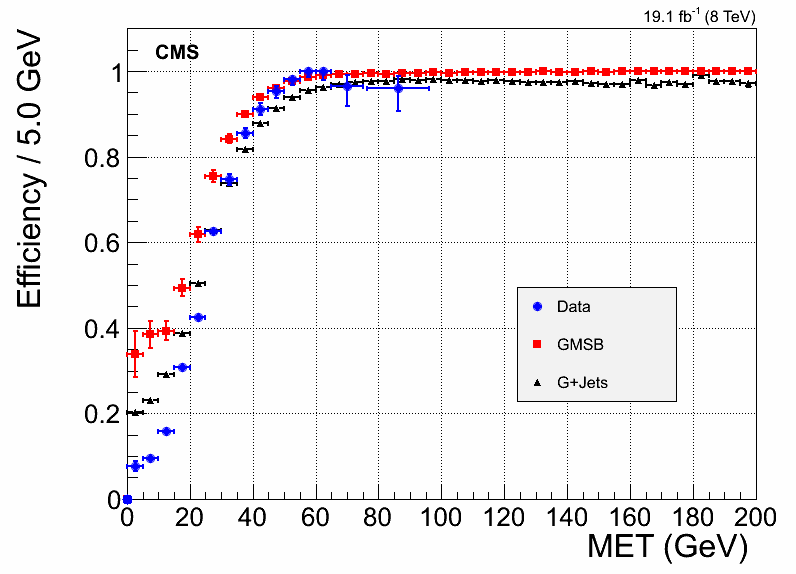
\includegraphics[height=0.55\textwidth, width=0.5\textwidth]{THESISPLOTS/PFMET_EffAsym.png}
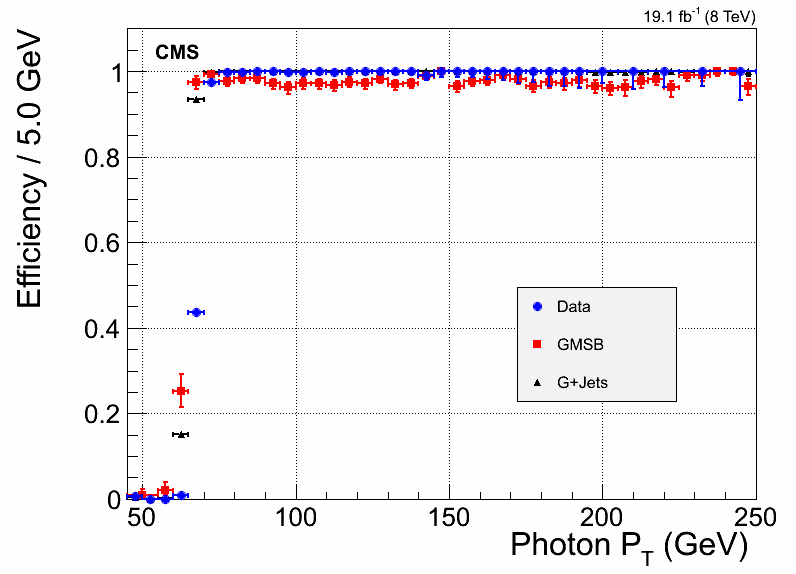
\includegraphics[height=0.55\textwidth, width=0.5\textwidth]{THESISPLOTS/Photon_EffAsym.png}}
\captionof{figure}{Our HLT efficiency turn-on curves in event \ETslash\hspace{0.15cm}~(left) and photon \pt~(right).The $\gamma +$jets samples require photon $\pt > 170$~\GeVc.}
\label{fig:HLTEff}
\end{center}
\end{minipage}
%%%%
\subsection{Offline Selection}
Our offline event selection, applied on the HLT triggered single photon events, require that the leading photon has $\pt > 80\GeVc$ and if the event has more than one photon, the sub-leading photon has $\pt > 45\GeVc$. Electromagnetic showers initiated by charged hadrons are rejected by requiring $E^{\mbox{\tiny{HCAL}}}/E^{\gamma} < 0.05$, where $E^{\mbox{\tiny{HCAL}}}$, is the sum of the energy in the HCAL towers directly behind the ECAL photon supercluster within a $\Delta R < 0.15$, with $\Delta R = \sqrt{(\eta - \eta^{\gamma})^{2} + (\phi - \phi^{\gamma})^{2}} $, and $E^{\gamma}$ is the photon energy in ECAL.
\newline 
Electrons are rejected by requiring the absence of hits in the first two layers of the pixel detector that is consistent with an electron track matching the observed location and energy of the photon candidate~(this is known as pixel veto requirement).
\newline
The photon candidates must satisfy three \textit{isolation} requirements that are designed to reject photons produced in hadronic decays:(1) $Iso_{\mbox{\tiny{TRK}}} < 0.2\GeV$, where $Iso_{\mbox{\tiny{TRK}}}$, is the sum of the \pt of tracks compatible with the primary event vertex in an annulus $0.015 < \Delta R < 0.40$, excluding a strip half $\eta$ width of 0.015 and the additional inner cone of size 0.04, optimized to exclude reconstructed tracks from $\PZ\rightarrow \EE$ events, centered around the line of vertex pointing to the photon supercluster. The exclusion is to remove the photon's own energy if it converts into an $\EE$ pair;
(2) $Iso_{\mbox{\tiny{ECAL}}} < 4.5\GeV$, where $Iso_{\mbox{\tiny{ECAL}}}$, is the transverse energy deposited in ECAL in an annulus  $0.045 < \Delta R < 0.4$, centered around the photon ECAL supercluster, excluding the strip half $\eta$ width of 0.02 and the additional inner cone of size 0.045 centered around the ECAL supercluster position; (3) $Iso_{\mbox{\tiny{HCAL}}} < 4.0\GeV$, where  $Iso_{\mbox{\tiny{HCAL}}}$ , is the transverse energy of HCAL tower in an annulus of $0.15 < \Delta R < 0.40$, centered about the ECAL supercluster position.
If the photon is very closed to a track within a range in $\Delta R(\gamma, track) < 0.6$, it is rejected. This is to avoid misidentifying charge particles as photons and to prevent double counting jets with high electromagnetic energy component as photons. The photon must also be isolated from any other particle in a cone size of $\Delta R(\gamma, \mbox{particle})< 0.4$.  The size of the photon electromagnetic shower along the minor axis~($S_{Minor}$) must be larger than 0.12 to suppress photons embedded in hadronic jets. 
\newline
Only photons belonging to the barrel~(EB) region \ie $|\eta_{\gamma}| < 1.479$ are accepted to avoid many out-of-time halo-induced photon candidates from ghost/satellite proton bunches, which belong to the endcap~(EE) shown in Figure \ref{fig:TIMEECAL}, and also since not many signal out-of-time photons go into the endcap.
\newline
Topological selection cuts, $1 - E_{6}/E_{2} < 0.98$ and $ 1 - E_{4}/E_{1} < 0.98$, on the photon energy deposit help suppress spikes.
A summary of our full photon selection criteria is presented in Table \ref{tab:PhotonSel}.
% which are caused by the direct interaction of the ECAL APDs by charged particles and neutrons producing anomalous photon signal
\newline
For jets, we select jets with $\eta_{jet} < 2.4$, and require that the main jet in the event has a $\pt > 35\GeVc$ with the event having at least 1 jet. This helps suppress non-collision background events without jets. The jets are reconstructed using the PF algorithm and identified based on the  identification selection criteria summarized in Table \ref{tab:JetSel}, where a jet candidate must satisfy the following: the Charge Electromagnetic Fraction~(CHF) and the Neutral Electromagnetic Fraction~(NEF) must make up a lesser portion of the jet sub-structure~($<99$\%), the Neutral Energy Fraction~(NEF) must be smaller than 99\%, to avoid misidentifying the jet as a photon. A jet near a photon object within a cone of 0.3 is rejected. 
\newline
We select events with missing transverse energy of at least 60\GeV for \ETslash\hspace{0.15cm} and ${\ETslash}^{\gamma}\hspace{0.15cm}$ as this is enough to suppress $\gamma + $jets and QCD events with false missing transverse energy.

\vspace{5mm}
\begin{minipage}{\linewidth} 
\begin{center}
\centering
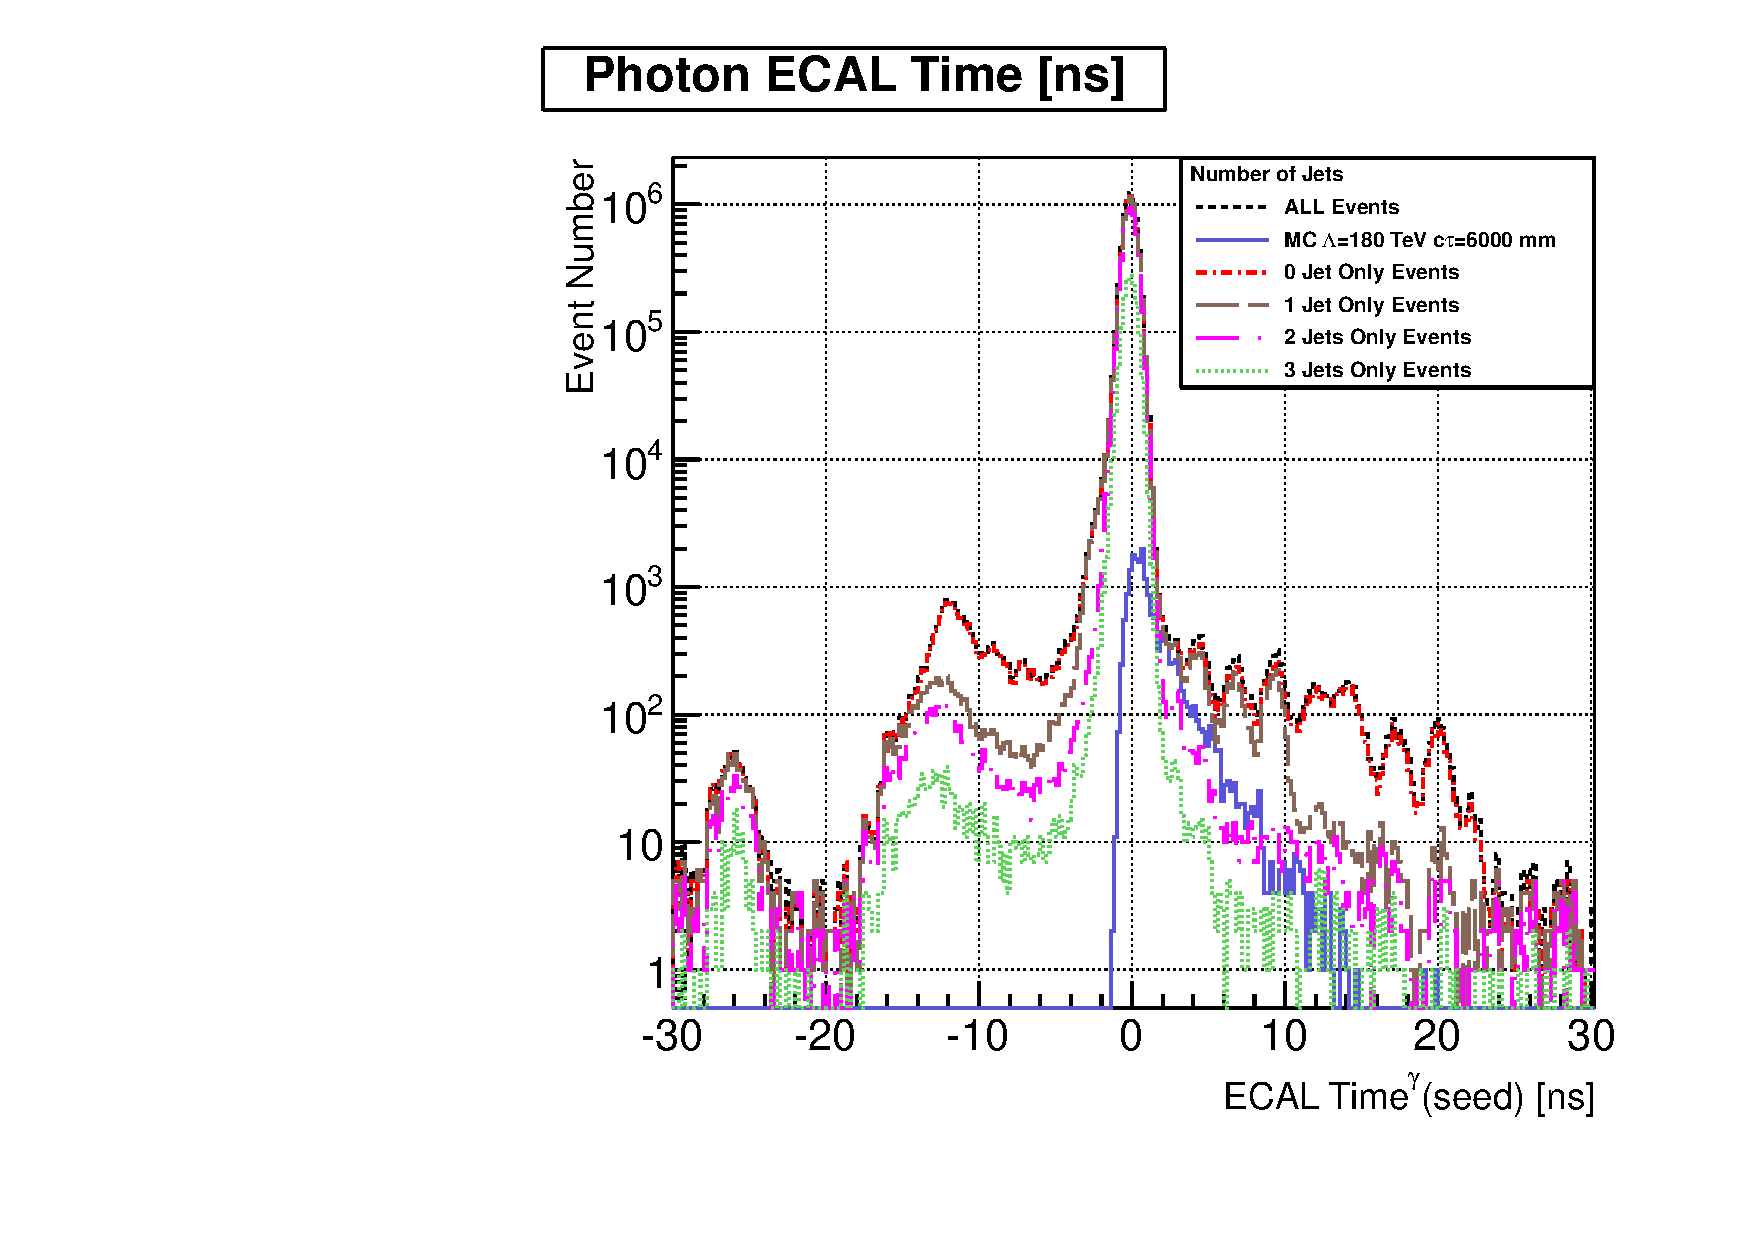
\includegraphics[height=0.65\textwidth, width=0.8\textwidth]{THESISPLOTS/Photon_SeedXtalTime_Distribution_VsJetMultiplicity.pdf}
\captionof{figure}{Comparing ECAL time distribution of events with different jet multiplicity from small sample of data and a single GMSB $\Lambda=180\TeV$ and $c\tau=6000$~mm sample. Accepted photons must have $\pt > 60$\GeV and belong to barrel and encaps.}
\label{fig:TimePlotJet}
\end{center}
\end{minipage}

\vspace{5mm}
\par
Looking at Figure \ref{fig:TimePlotJet}, we find that most of our background events with out-of-time beam halo-induced photons are mostly zero- and one-jet events. As a result, we use these zero and one jet events as a control sample only to study our background events, while our signal-like events are events with the following topology: $\ge1~\gamma + \ge2~ jets + \ETslash\hspace{0.15cm} > 60\GeV + {\ETslash}^{\gamma}\hspace{0.15cm} > 60\GeV$. 


\clearpage

\vspace{5mm}
\begin{minipage}{0.85\linewidth} 
\begin{center}
%\begin{table}[ht]
\begin{tabular}{l c }
\toprule
\hline
\multicolumn{2}{l}{\bfseries{Photon Selection Criteria}} \\
  \hline 
  \bfseries{Criteria} & \bfseries{Requirement} \\
   \hline 
   \toprule
 % \texttt{primary vertex number of tracks(vnof)}& $>= 4$ \\
 % \texttt{primary vertex transverse distance to beam}~($d0$) & $ < 2$~cm from CMS center \\
%  \texttt{primary vertex longitudinal distance to beam}~($|z|$) & $ < 24$~cm from CMS center \\
  \texttt{Event leading photon must have} $\pt(\gamma^{1})$  & $ > 80\GeV$ \\
  \texttt{Other photons in event must have} $\pt(\gamma^{2,3,...})$  & $ > 45\GeV$ \\
 $|\eta_{\gamma}|$,(\texttt{Barrel Only}),  & $ < 3.0$ ($ < 1.5$) \\
 $S_{Minor}$  & $ 0.12 \leq S_{Minor} \leq 0.38$ \\
 $E^{\mbox{\tiny{HCAL}}}/E^{\gamma}$  & $ < 0.05$ \\
 $\Delta R(\gamma, track)$  & $ > 0.6 $ \\
 $Iso_{\mbox{\tiny{HCAL}}}$, $Iso_{\mbox{\tiny{ECAL}}}$, $Iso_{\mbox{\tiny{TRK}}}$  & $ < 4.0\GeV $, $ < 4.5\GeV $, $ < 0.2\GeV $ \\
 Photon Isolation cone size $\Delta R(\gamma, \mbox{particle})$ & $< 0.4$ \\
 Topological Spike cuts  & $1 - E_{6}/E_{2} < 0.98$, $ 1 - E_{4}/E_{1} < 0.98$ \\ 
  \hline 
  \bottomrule
\end{tabular}
\captionof{table}{The photon identification and selection  criteria used in this analysis}
\label{tab:PhotonSel}
%\end{table}
\end{center}
\end{minipage}

\vspace{10mm}
\begin{minipage}{0.85\linewidth} 
\begin{center}
%\begin{table}[ht]
\begin{tabular}{l c }
\toprule
\hline
\multicolumn{2}{l}{\bfseries{Jet PF identification selection criteria}} \\
  \hline 
  \bfseries{Criteria} & \bfseries{Requirement} \\
   \hline  
   \toprule
\texttt{Jet} \pt & $ > 35$\GeV \\
 \texttt{Number of Jet constituents} & $ > 1$ \\
 \texttt{Charge EM energy fraction~(CEF) } & $ < 0.99$ \\
 \texttt{Neutral Hadron energy fraction~(NHF) } & $ < 0.99$ \\
 \texttt{Neutral EM energy fraction~(NEF) } & $ < 0.99$ \\
 \texttt{If} $|\eta|$ \texttt{of jet is} $ >2.4$, \texttt{Charge Hadron energy fraction~(CHF) } & $ > 0$ \\
 \texttt{If} $|\eta|$ \texttt{of jet is} $ >2.4$, \texttt{Charge multiplicity~(NCH) } & $ > 0$ \\
 $\Delta R(\gamma, jet) = \sqrt{(\phi_{\gamma}-\phi_{jet})^{2} + (\eta_{\gamma}-\eta_{jet})^{2}}$ & $ > 0.3$ \\
 \toprule
 \texttt{\ETslash \hspace{0.25cm}, ${\ETslash}^{\gamma}\hspace{0.15cm}$} & $ > 60\GeV$ \\
\hline
\bottomrule
\end{tabular}
\captionof{table}{The Jet ID and MET selection used in this analysis}
\label{tab:JetSel}
%\end{table}
\end{center}
\end{minipage}

\clearpage
%%%$$$

\section{Background Estimation}
Most of our background events with out-of-time photons are non-collision events produced from  different sources. In order to qualify and quantify these different sources, we compare in-time~($|t_{\gamma}| < 2$\ns) photon candidates to out-of-time~($t_{\gamma} < -3$~ns and $t_{\gamma} > 3$\ns) photon candidates.
By also comparing photons from events with different number of jets, we were able to uncover the different background sources and better quantify the contribution from each source. In Figure \ref{fig:BKGPLOTS}, we present scatter plots of the photon's ECAL time against $\eta$~(left) and against $\phi$~(right) for events with $\ETslash\hspace{0.25cm} > 25\GeV$ and photon $\pt > 60\GeV$, belonging to the barrel and endcap regions.

\vspace{5mm}
\begin{minipage}{0.95\linewidth} 
\begin{center}
\centering
\mbox{
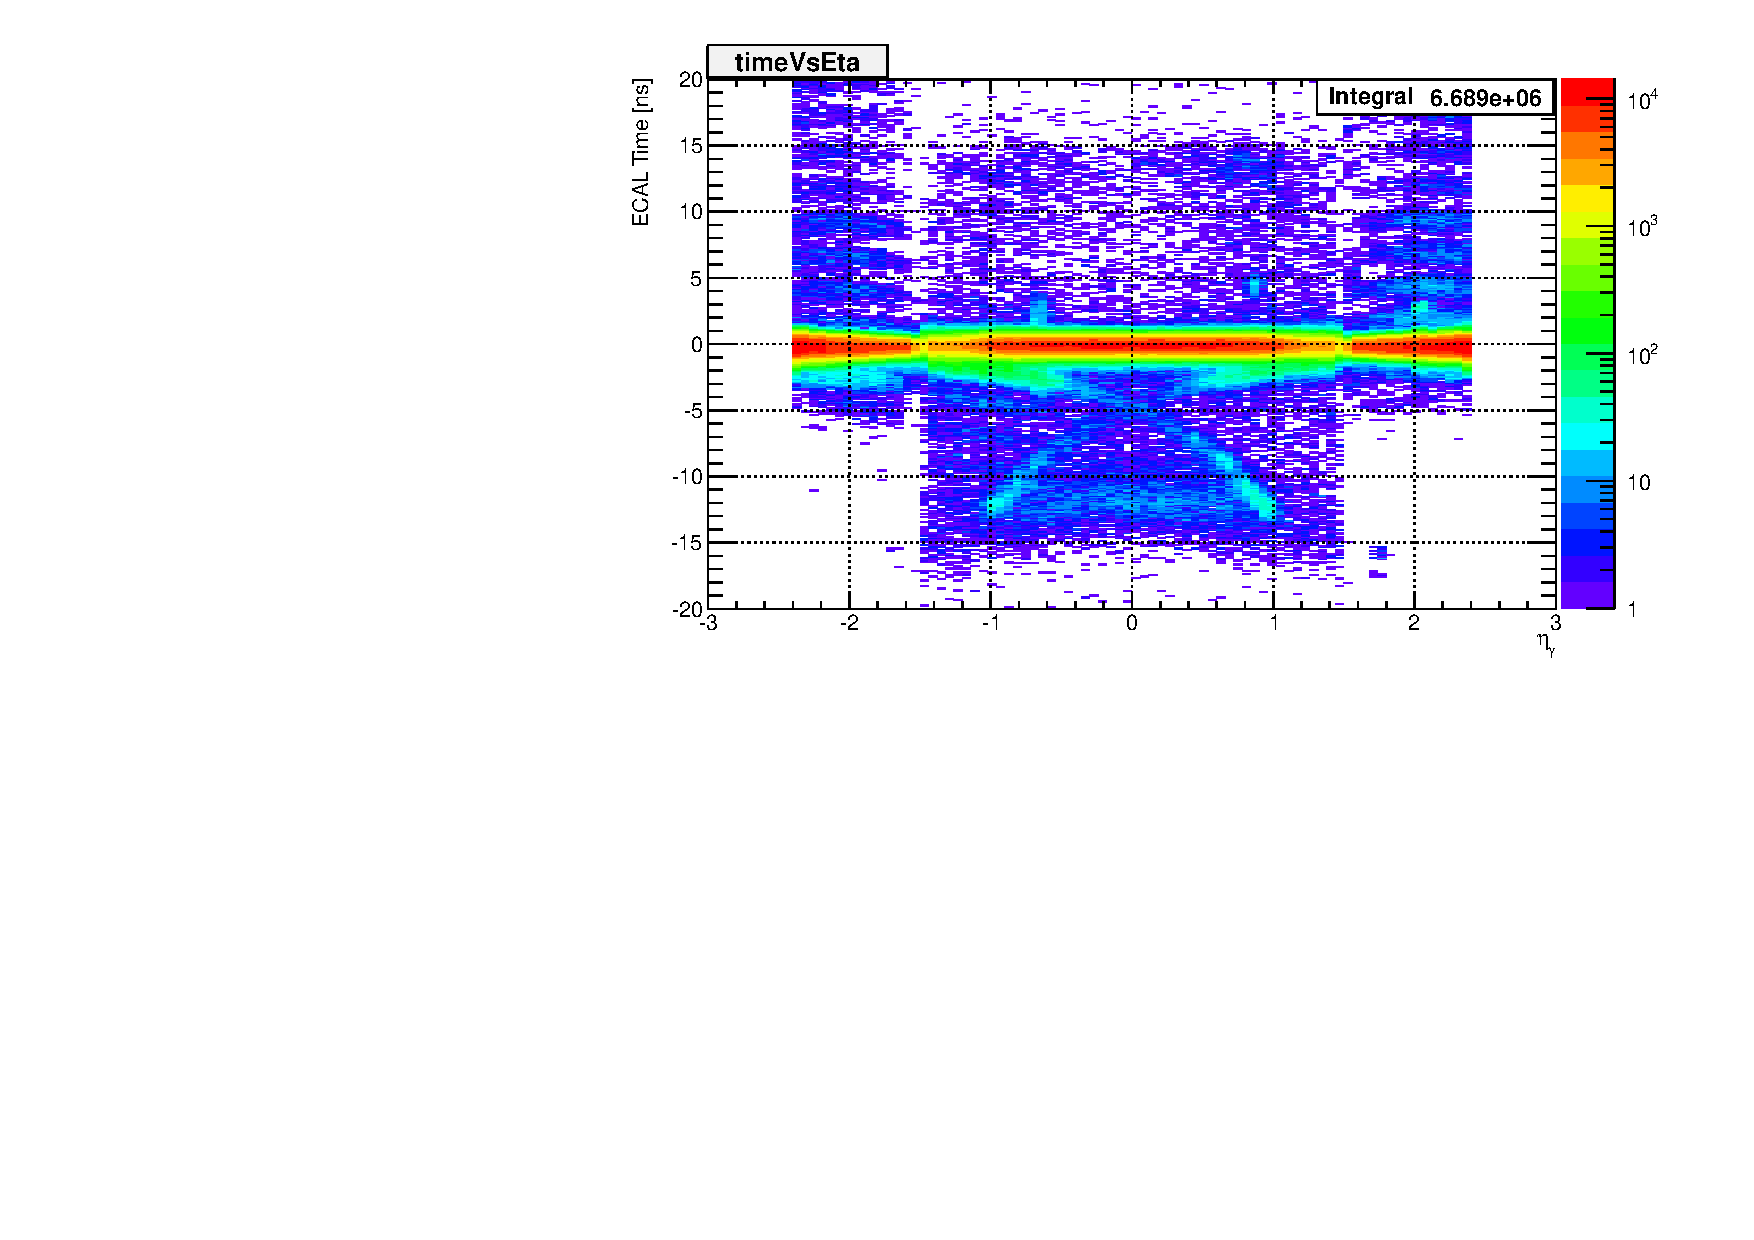
\includegraphics[height=0.55\textwidth, width=0.5\textwidth]{THESISPLOTS/SinglePhotonDataSet-TimeVsEta.pdf}
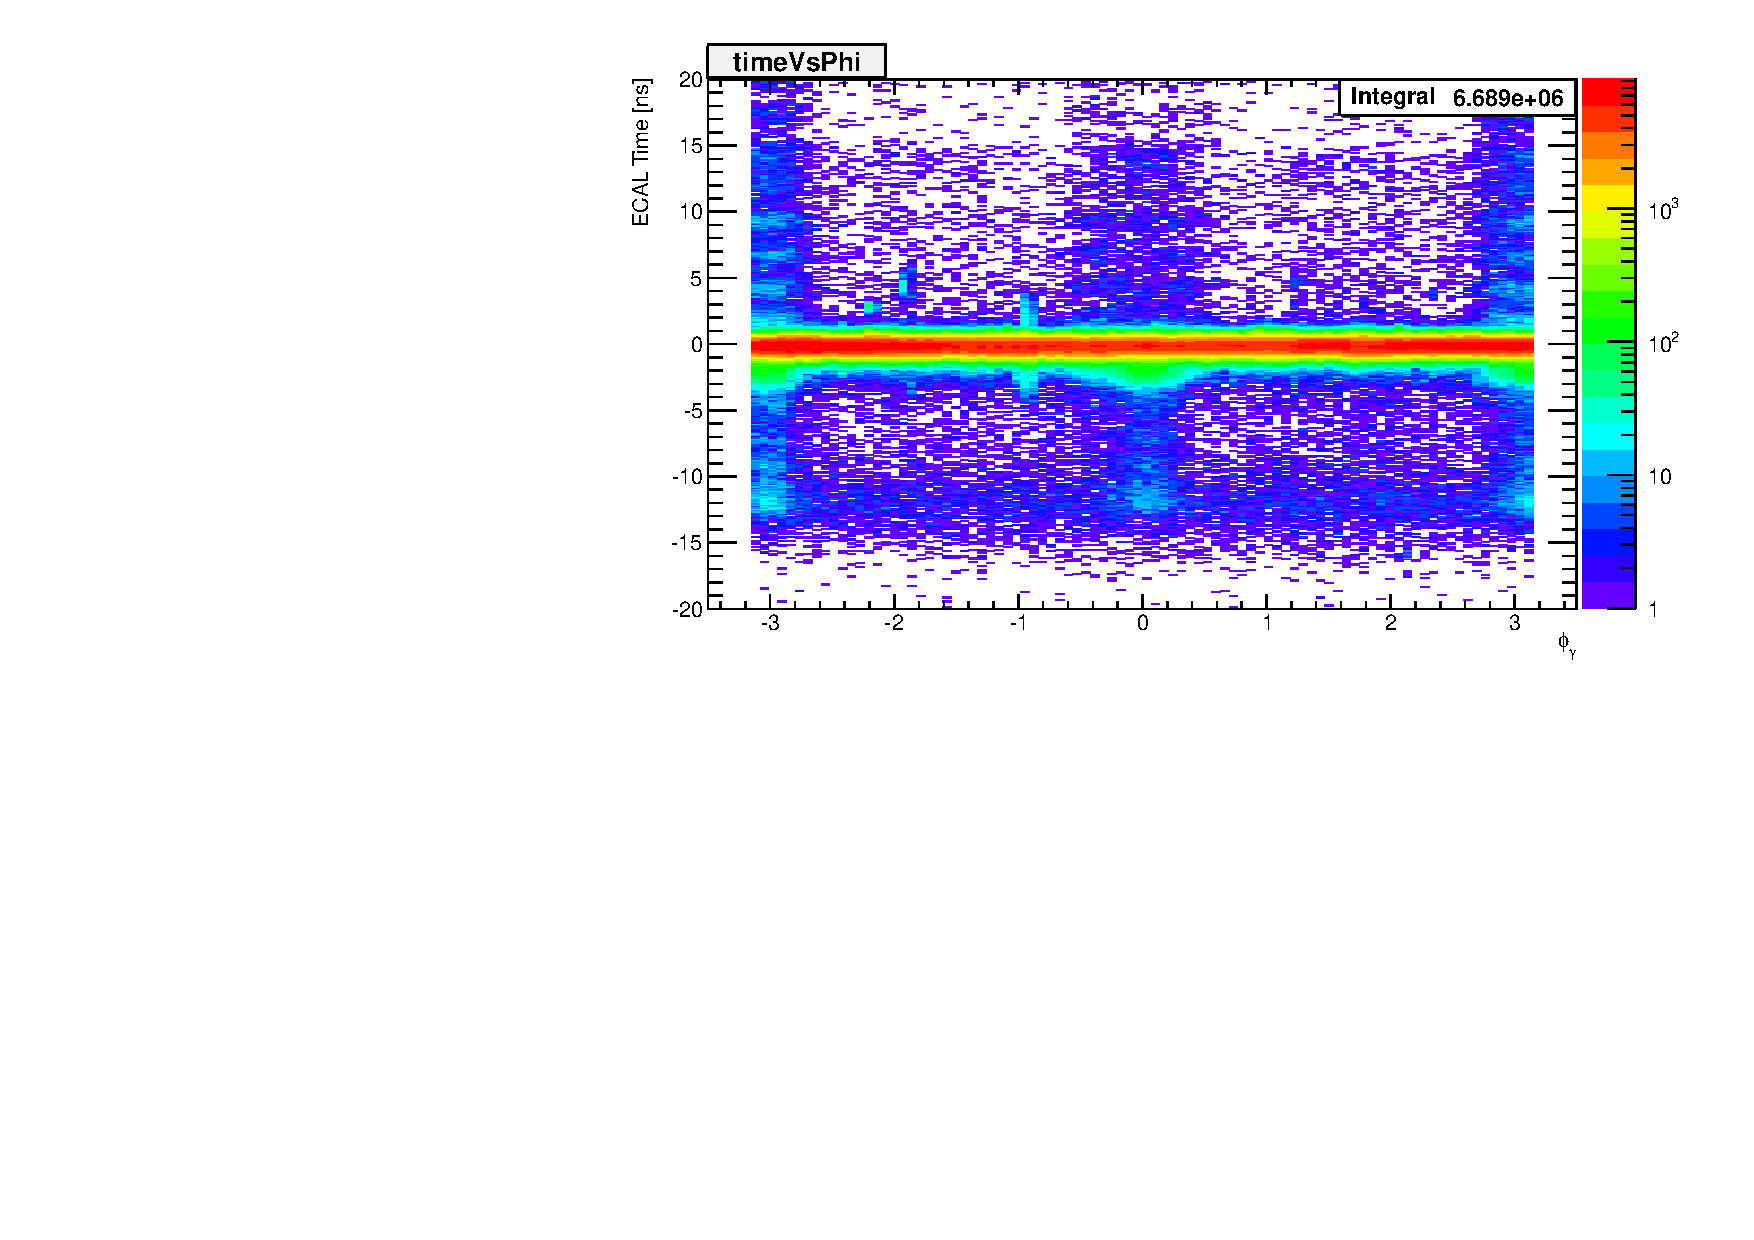
\includegraphics[height=0.55\textwidth, width=0.5\textwidth]{THESISPLOTS/SinglePhotonDataSet-TimeVsPhi.pdf}}
\captionof{figure}{ECAL time against $\eta$~(left) and ECAL time against $\phi$~(right) for photons with $\pt > 60$\GeV from data.}
\label{fig:BKGPLOTS}
\end{center}
\end{minipage}

\vspace{5mm}
These scatter plots show that a good number of photons that are out-of-time belong to very different sources. For example, the "cross-like" feature seen on the left plot, is particular to photons with earlier time and in combination with the time-discrete pattern, prominent in the endcaps~($1.479 < \eta_{\gamma} < 3$) regions and the high concentration at $\phi=0\pm\pi$ on the plot on the right, can be interpreted as photons produced by the so-called proton beam halo. We argue the background out-of-time photon candidates can be split into 4 major categories: (1) Halo-induced photons from main and satellite beam halo muons, because they have early or late arrival times, creates the cross-like feature and time-discrete pattern and are also highly concentrated at $\phi=0,\pm\pi$, (2) Cosmic-induced photons produced from cosmic muons since the arrival time in ECAL is random, (3) Spikes, due to the high concentration of photons with time of about -12.5\ns and Finally, (4) Collision background events with photons with mis-measured ECAL time.
\newline
Since spikes are notoriously difficult to identify and eliminate, to reduce their contribution to out-of-time photons, we restrict our event selection to photons with time $ 2.0 < t_{\gamma} < 13.0$\ns and $-10.0 < t_{\gamma} < -3$\ns. This reduces our signal search window for events with late photon time to events with the photon time between $2.0 < t_{\gamma} < 13.0$\ns.
\par 
We split the background events into Collision and Non-Collision event categories and study each category separately. We first identify and reject photon candidates from beam halo, cosmic muons and spikes and then estimate the residual non-collision and collision background photon candidates  using the \textbf{\textsf{ABCD}} background estimation technique. 

\subsection{Collision Background}
\subsubsection{Collision Background Photons}
Events from satellite proton bunches described in section \ref{Ghost}, produce out-of-time photons which can be present in the barrel. We refer to the events from collisions with out-of-time photons, including QCD events with photons which have mis-measured time, as our \textit{Collision background} events. It is challenging to define a strategy for rejecting this background events. Our approach, after rejecting non-collision events, is to estimate their contribution to signal using the \textsf{ABCD} background estimation method. We also perform a separate background estimation using a control sample of \PZ events and show that these events with out-of-time photons are events from collision with photon candidates with mis-measured time or from satellite proton bunches.
% We elaborate more on this in the collision background estimation section.%We will More on this is discussed in future sections.
%%%%
\subsection{Non-Collision Background}
%We study non-collision background events from beam halo muons, cosmic muons, and spikes using a data sample of zero and one jet events passing all our event selection requirements.
% These events consist of have photons with large reconstructed time and large \ETslash\hspace{0.15cm} measurements. The high \pt photons from these energetic muons and possible overlapping  pile up events from multiple $pp$ collisions, contribute to the total sum of the PF reconstructed \pt imbalance leading to their large \ETslash\hspace{0.15cm} and at times jets associated with these events.
%We select events with at least one good vertex, zero or one jet, photons satisfying ECAL spike cleaning, associated with candidate muons satisfying DT time cosmic muon cleaning and CSC tight halo-muon cleaning requirements to study these non-collision events. 
%A schematic diagram in Figure \ref{fig:NeutDecay} show the production of photons from both non-collision and collision{ghost/satellite} in a typical LHC $pp$ collision within the CMS detector. Also shown is a typical photon from a neutralino decay in the GMSB model. Still on the diagram is shown the point of entry of beam halo muons into the CMS detector comparing to what is observed in the photon ECAl time against $\eta$ and $\phi$ plots of Figure \ref{fig:BKGPLOTS}.

%\vspace{5mm}
%\begin{minipage}{0.90\linewidth} 
%\begin{center}
%\captionsetup{type=figure}
%\mbox{
%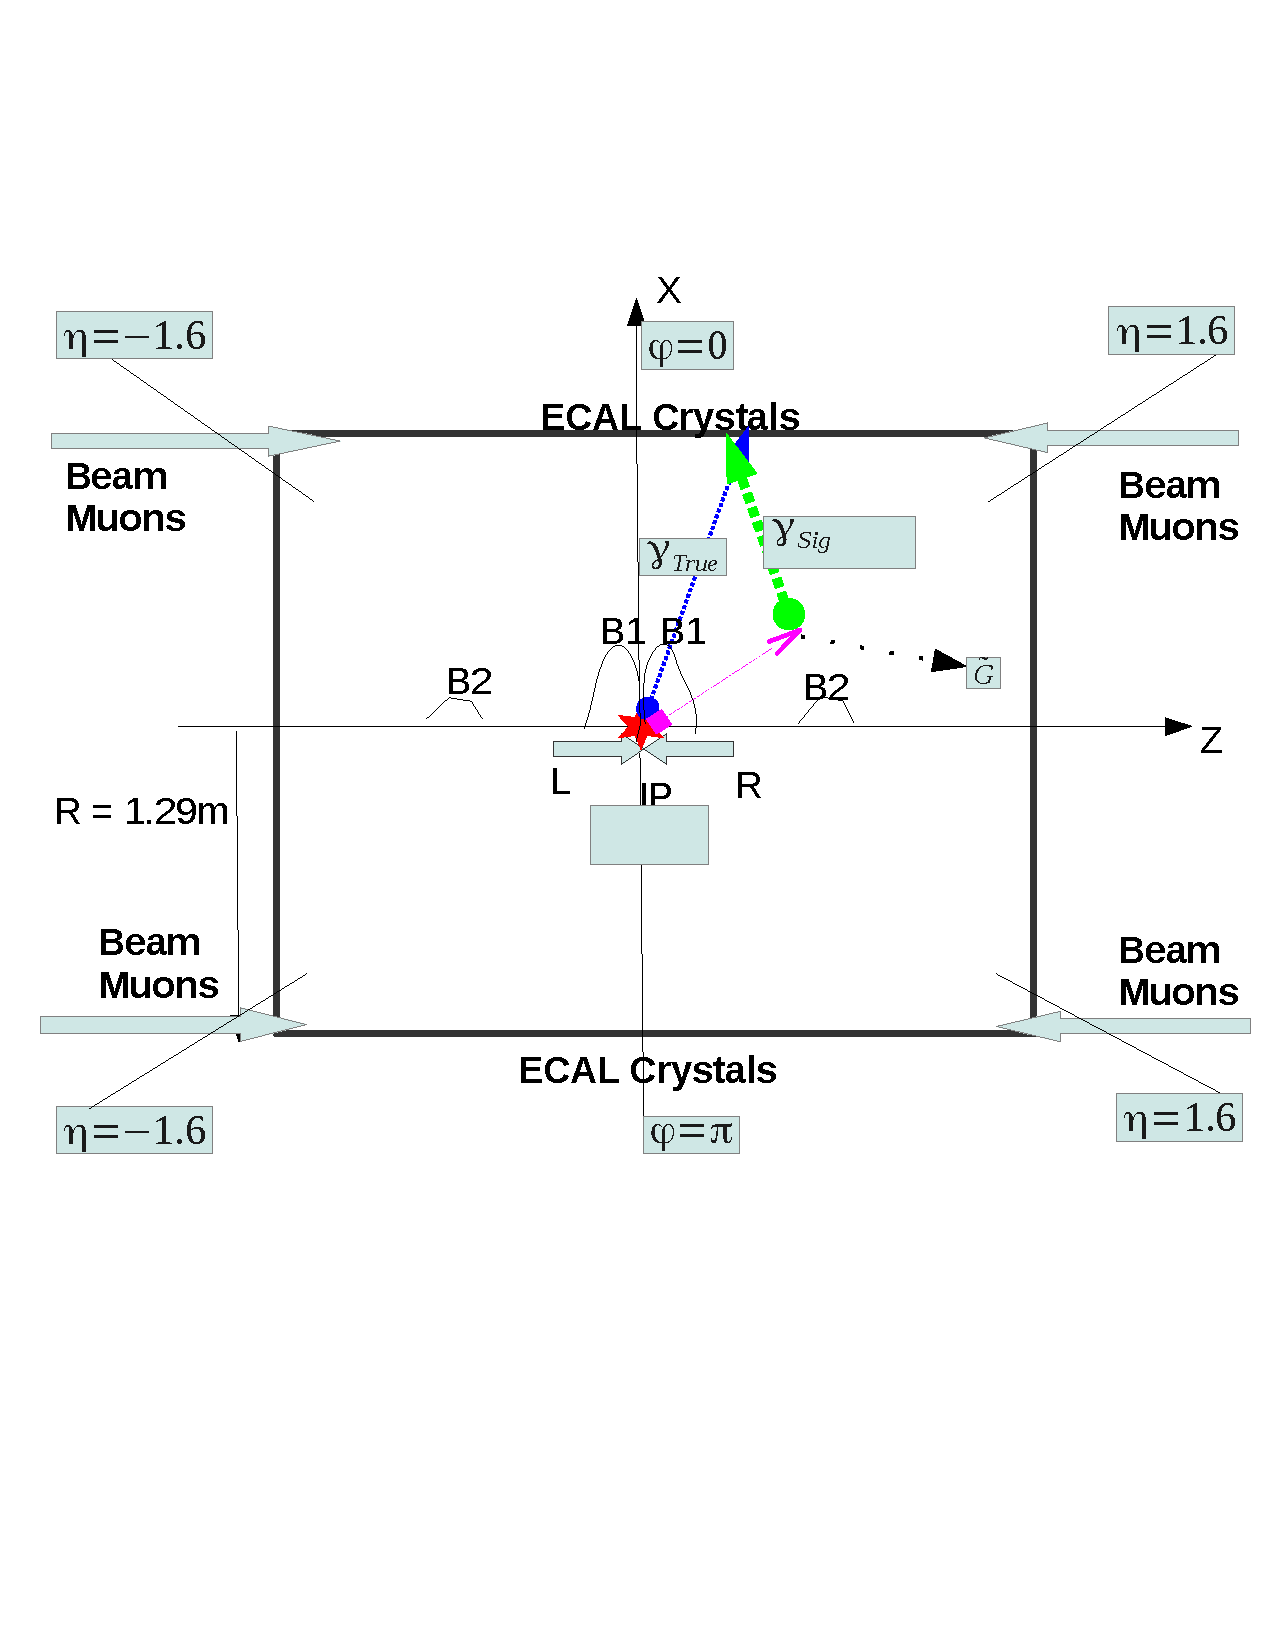
\includegraphics[height=0.35\textwidth, width=0.5\textwidth]{THESISPLOTS/Background_Delayed_Photon.pdf}}
%\captionof{figure}{Schematic diagram showing production of photons from main $pp$ and possible ghost/satellite bunch collisions in the CMS detector volume. Typical beam halo muon's entry direction into ECAL and GMSB neutralino decay is shown.}
%\label{fig:NeutDecay}
%\end{center}
%\end{minipage} 
%%%%%

\subsubsection{Halo-induced Photons}
Protons in the main and sometimes satellite bunches can, through inelastic scattering with residual gas molecules like $\mbox{H}_{2}$ and C$\mbox{O}_{2}$ in beam pipe, produce pions which later decay into muons traveling with energy of a few \TeV, called \textit{Beam Halo} muons. These energetic muons often radiate energetic photons called \textit{Halo-induced photons} in the calorimeter through a process called \textit{bremsstrahlung}. Some of the beam halo muons are produced when protons scatter off Tertiary Collimators~(TCT), $50\m < z < 148$\m, away from the center of the CMS detector.
%, due to proton beam small angle scattering with gas
These halo muons travel nearly parallel to the main proton bunch but sometimes steer outward from the nominal orbit due to betatron oscillations, in the transverse direction spreading mostly in the horizontal plane. Despite beam cleaning, a sizable population of beam halo muons remains and eventually produce energetic photons in the calorimeters. A scatter plot of the photon ECAL time against $\phi$  shown earlier in the right plot of Figure \ref{fig:BKGPLOTS}, shows that most of these beam halo muons enter the ECAL in the horizontal plane at $\phi=0,\pm\pi$. The rate of halo-induced photons depend on the beam intensity, beam current and the operational conditions of the LHC, like, the  machine optics, collimator settings, residual gas densities and LHC proton filling scheme. 
\newline
The halo muons before entry into ECAL produce track hits which can be reconstructed into muon track segments in the Cathode Strip Chambers~(CSC) Endcap muon detectors. The reconstructed track hits in the CSC segments can be associated with a halo-induce photon supercluster in ECAL within some narrow angular range in $\phi$.
\newline
Most of the halo muons end up in the endcaps but some can also end up in the barrel. The resulting halo-induced photons are usually out-of-time. All of halo-induced photons have early arrival time compared to photons produced directly from nominal $pp$ collisions since the path travel by the beam halo muons to arrive at the crystals in ECAL is shorter than for the protons in the main bunch. The halo-induced photon's arrival time can be estimated from the unique flight path of the beam halo muons with respect to the arrival time of photons from $pp$ collisions as 
\begin{equation}{\label{eq:HALOPATH}}
t^{\mbox{expected}}_{\mbox{ECAL}} = -1/c\left( \pm Z_{\mbox{cluster}} + \sqrt{Z^{2}_{\mbox{cluster}} + R^{2}_{\mbox{cluster}}}  \right),
\end{equation}
where $Z_{\mbox{cluster}}$ is the $Z$ coordinate of the point where the halo muon hit ECAL, $R$ is the radial distance of the supercluster from the beam line, which is equal to $1.29$\m in the barrel, and $c$ is the speed of light in vacuum. The estimated halo-induced photon arrival time can be re-arranged to become
\begin{equation}{\label{eq:HALOPATH2}}
t^{\mbox{expected}}_{\mbox{ECAL}} = - \frac{R}{2c} \exp^{(-\eta)},
\end{equation} 
showing the direct dependence on $\eta$. In Figure \ref{fig:HALO}, the halo-induced photon estimated time is shown by the two red lines, agreeing well with observation from data. This give us confidence that we understand the source of halo-induced photons and can develop a method of identifying events with halo-induced photons. By matching halo muon hit positions in $\phi$ in CSC segments to photon supercluster positions in ECAL, we are able to match halo muons to their corresponding halo-induced photons. We use the quantity, $\Delta\phi(\mbox{CSC Seg},\gamma)$, which is defined as the difference in $\phi$ between the CSC segment  and the photon supercluster position in ECAL, to express this matching. A plot of $\Delta\phi(\mbox{CSC Seg},\gamma)$ for in-time and out-of-time photons is shown in the left plot of Figure \ref{fig:HALO}. We find that out-of-time photons often have small $\Delta\phi(\mbox{CSC Seg},\gamma)$, further confirming that some out-of-time photons are produced by beam halo muons.

\vspace{5mm}
\begin{minipage}{0.95\linewidth}  
\begin{center}
%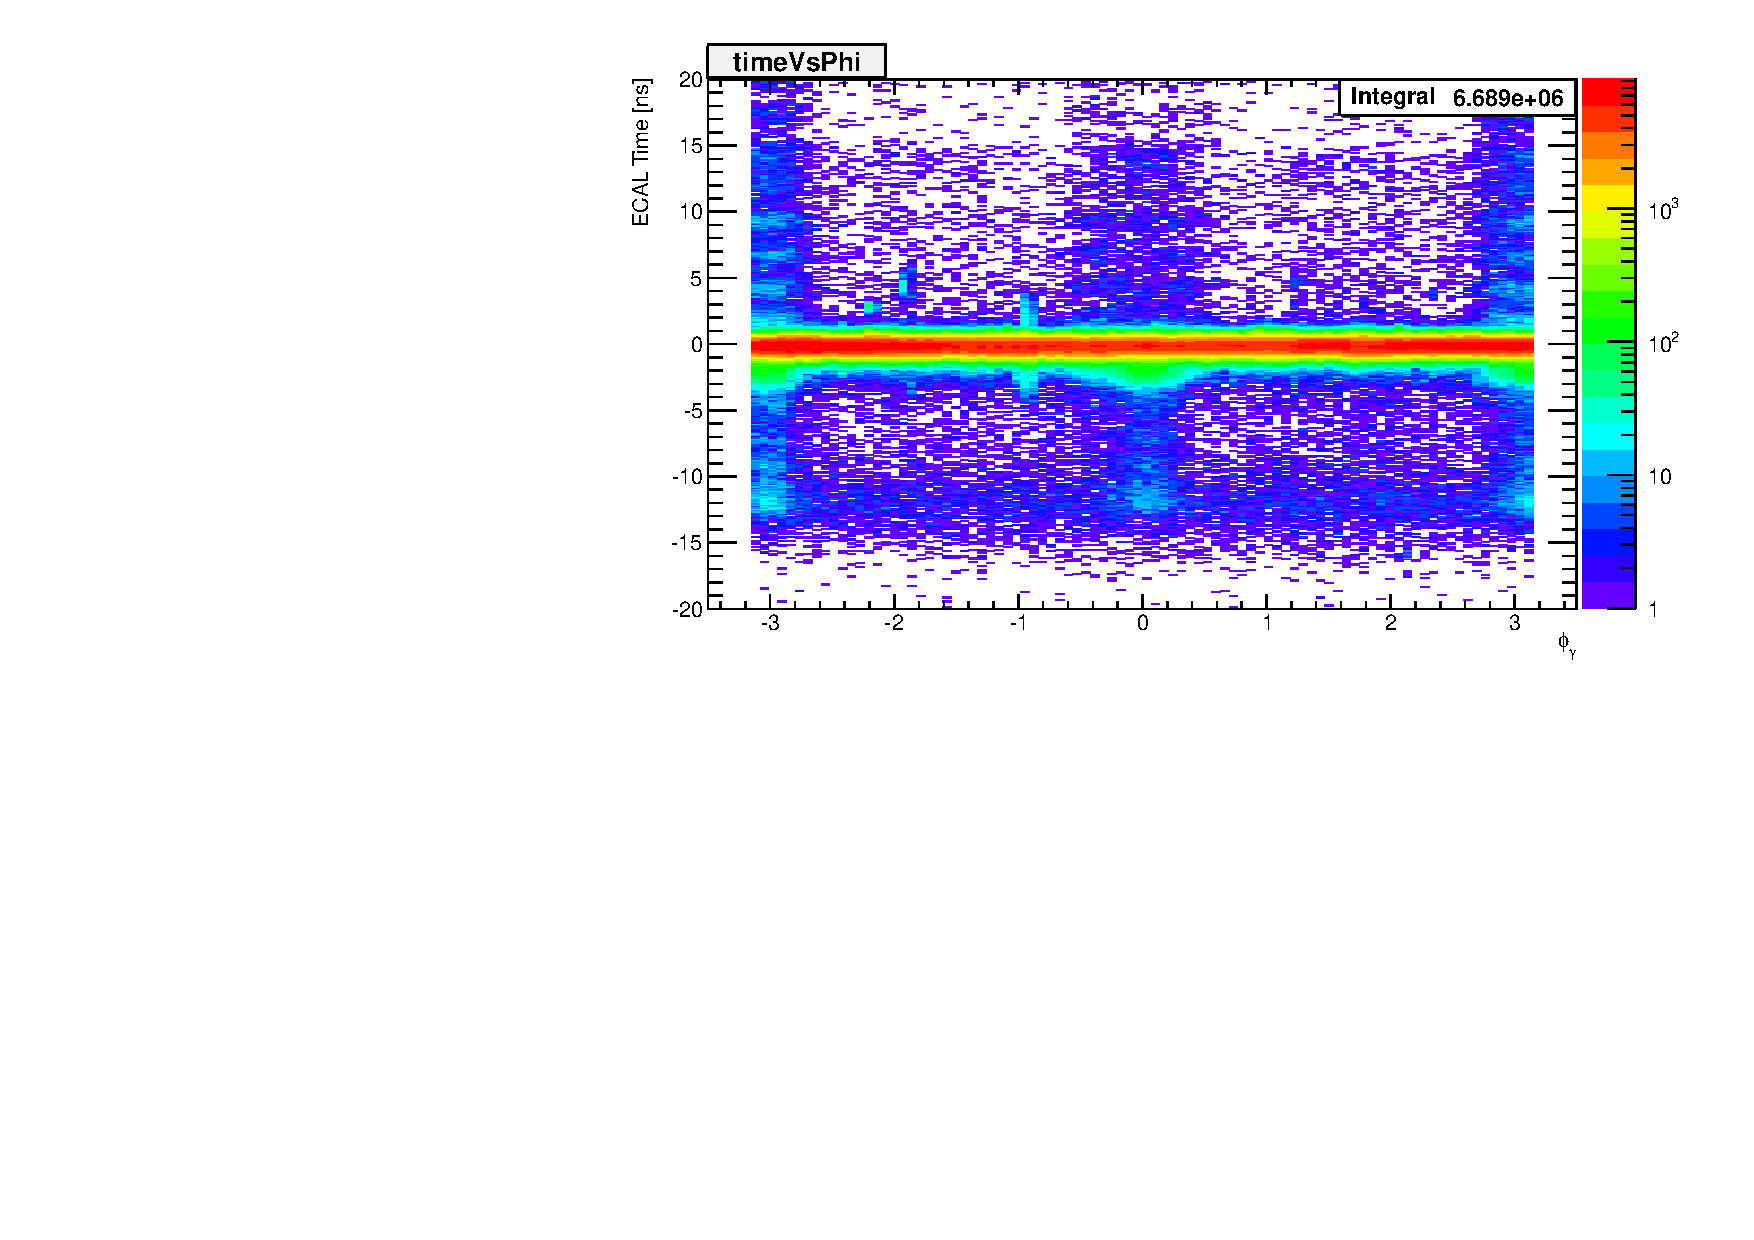
\includegraphics[height=0.35\textwidth, width=0.5\textwidth]{THESISPLOTS/SinglePhotonDataSet-TimeVsPhi.pdf}}
\mbox{
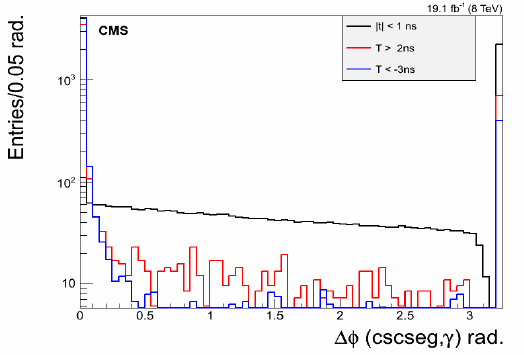
\includegraphics[height=0.5\textwidth, width=0.5\textwidth]{THESISPLOTS/CSC-Segment-Halo-Tagging.png}
%{THESISPLOTS/CSC_Segment_Halo_data.png}
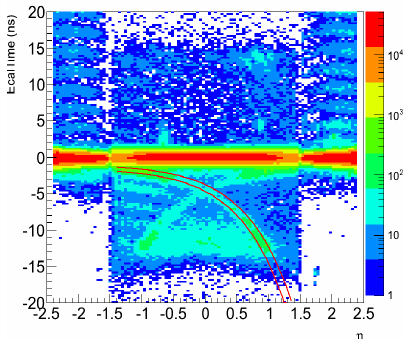
\includegraphics[height=0.5\textwidth, width=0.5\textwidth]{THESISPLOTS/HALO-ECAL-TIME-Vs-ETA.png}}
\captionof{figure}{ECAL time $vs$ $\Delta\phi(\mbox{CSC Seg},\gamma)$~(left)  for in time~(black) and out-of-time~(red and blue) photons. Photon ECAL time $V.s$ $\eta$~(right), expected halo-induced photon time is shown as two red lines.}
\label{fig:HALO}
\end{center}
\end{minipage}

%\vspace{5mm}
%%% Tagging Halo in EB is non-trivial!!! So no dicussion
%To estimate the performance of using $\Delta\phi(\mbox{CSC Seg},\gamma)$ for tagging events with halo photons, we use a halo-induced photon candidate sample of selected events with photons in the endcaps where we expect mostly halo photon candidates and with $\phi_{\gamma}$ around $\phi = 0, \pm \pi$. We were able to tag with $\Delta\phi(\mbox{CSC Seg},\gamma) < 0.05$, a good number of photon candidates as halo-induced photons in the endcaps shown in the Figure \ref{fig:HALOENDCAP} comparing halo-induced photons in the endcaps to tagged halo photons in the endcaps.
% 
%\begin{minipage}{0.90\linewidth} 
%\begin{center}
%\centering
%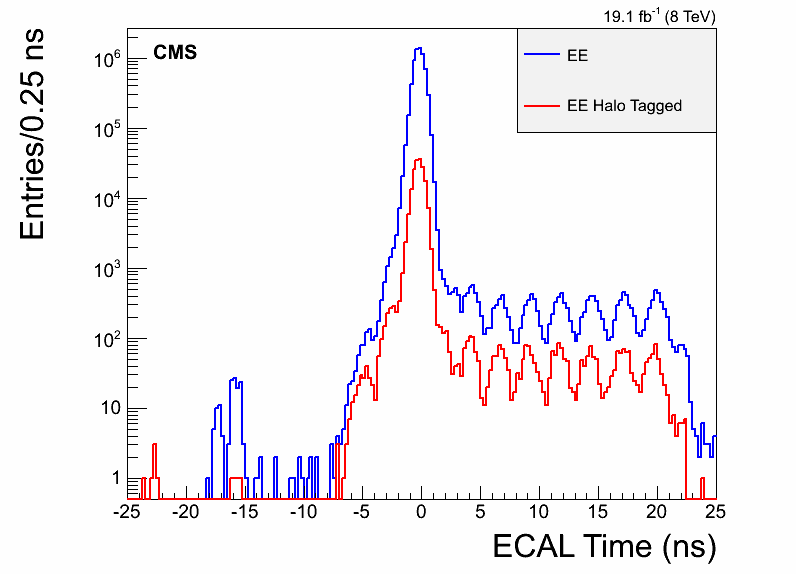
\includegraphics[height=0.45\textwidth, width=0.7\textwidth]{THESISPLOTS/halo_EE_Time.png}
%\captionof{figure}{Using $\Delta\phi(\mbox{CSC Seg},\gamma) < 0.05$ to tag photons with $\phi_{\gamma} = 0, \pm \pi$ in the endcaps. A good portion of endcap photon candidates are tagged.}
%\label{fig:HALOENDCAP}
%\end{center} 
%\end{minipage}

\subsubsection{Cosmic-induced Photons} 
Muons produced in cosmic rays with sufficient energy, traveling through the CMS detector, will radiate~(bremsstrahlung) photons in ECAL. We refer to these photons as \textit{cosmic-induced photons}. Unlike halo muons, muons from cosmic rays can arrive at ECAL from any direction at any time. We expect the cosmic-induced photons in the barrel to leave track segments in the Drift Tubes~(DT) behind the calorimeters.
\newline
 Using these DT segments and  photon supercluster position in ECAL we can match cosmic muon DT segments to ECAL photon superclusters within a narrow window in $\Delta\eta$ and $\Delta\phi$. In reality, because of the large space between the muon barrel and the ECAL we calculate the projected position of the muon segment at the outer surface of ECAL using the direction of the DT segment and use the projected position to calculate $\Delta\eta$ and $\Delta\phi$. A scatter plot for $\Delta\eta(\mbox{DT Seg},\gamma)$ and $\Delta\phi(\mbox{DT Seg},\gamma)$ of the matching for events with out-of-time photons~($t_{\gamma} > 2$\ns and $t_{\gamma} < -3$\ns) is shown on the right plot of Figure \ref{fig:COSMIC}. We compare these scatter plots of $\Delta\eta(\mbox{DT Seg},\gamma)$ and $\Delta\phi(\mbox{DT Seg},\gamma)$ to the scatter plots for in-time~($|t_{\gamma}| < 1$\ns) shown on the left plot of the same Figure \ref{fig:COSMIC} and find that a large fraction of the out-of-time photons have a small $\Delta\eta$ and $\Delta\phi$. 
 \newline
Comparing these scatter plots of $\Delta\eta$  and $\Delta\phi$ for these out-of-time photons to the scatter plots for cosmic-induced photons from a pure cosmic muons sample~(data recorded by the CMS detector in the absence of proton-proton collisions) shown in Figure \ref{fig:TRUECOSMIC}, we find a similar small $\Delta\eta$ and $\Delta\phi$ occupancy for the true cosmic muons events from the pure cosmic sample. We conclude the following: it is possible to use small $\Delta\eta(\mbox{DT Seg},\gamma)$  and $\Delta\phi(\mbox{DT Seg},\gamma)$ to identify and reject events with cosmic-induced photons.

\vspace{5mm}
\begin{minipage}{0.95\linewidth} 
\begin{center}
\mbox{
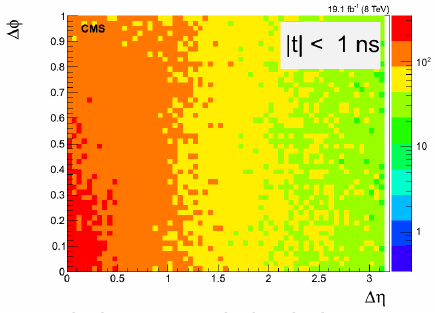
\includegraphics[height=0.5\textwidth, width=0.5\textwidth]{THESISPLOTS/Cosmic_In-time-Photons_Data.png}
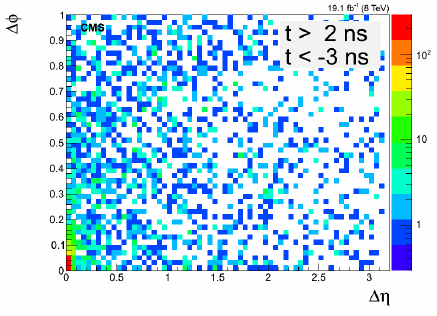
\includegraphics[height=0.5\textwidth, width=0.5\textwidth]{THESISPLOTS/Cosmic_Out-Of-time-Photons_Data.png} 
}
\captionof{figure}{Scatter plot showing $\Delta\eta(\mbox{DT Seg},\gamma)$ against $\Delta\phi(\mbox{DT Seg},\gamma)$ for out-of-time~($ t_{\gamma} > 2$~ns and $t_{\gamma} < -3$~ns) photons~(right) compared to in-time($|t_{\gamma}| < 1$~ns) photons~(left). Cosmic photon candidates have small $\Delta\eta$ and $\Delta\phi$.}
\label{fig:COSMIC}
\end{center}
\end{minipage}

%\paragraph*{}\mbox{}\\
\begin{minipage}{0.90\linewidth} 
\begin{center}
\mbox{
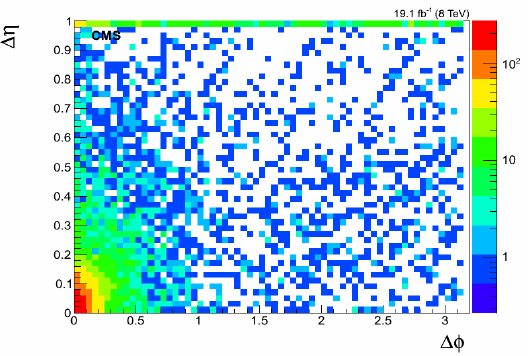
\includegraphics[height=0.45\textwidth, width=0.6\textwidth]{THESISPLOTS/Cosmic_Ray_Photons_Cosmic_dataset.png} }
\captionof{figure}{Scatter plot of $\Delta\eta(\mbox{DT Seg},\gamma)$ against $\Delta\phi(\mbox{DT Seg},\gamma)$ for photons from pure cosmic muon data. Small $\Delta\eta$ and $\Delta\phi$ are cosmic photons.}
\label{fig:TRUECOSMIC}
\end{center}
\end{minipage}


%By looking at the signal pulse height, the pulse shape for a spike signal appear different from a signal form an electromagnetic particle. Because of this difference in pulse shape profile, the reconstructed ECAL time for spikes usually have large calculated $\chi^{2}$~(defined in Equation \ref{eq:CHI2})  values.
\subsubsection{Spike-Seeded Photons}
Neutrons and charge hadrons can at times deposit their energy directly unto the APDs instead of through the crystal scintillation process. Such APD signals are \textit{anomalous} and are unfortunately reconstructed as photons called \textit{spike-seeded photons} or simply \textit{spikes}. Spikes produced from $pp$ collisions can pass our photon selection requirements and be mistakenly identified as good photon candidates. A spike supercluster usually consist of very few crystals; most often one or two crystals. However, they can sometimes overlap with good photon candidates or buried inside jets. Such embedded spikes cannot be easily identified. 
\newline
The arrival time of spikes is much earlier~(negative), usually about $t = -12.0$\ns, than for photons produced in nominal $pp$ collisions and depositing their energy through crystal scintillation. This is because for spikes there is the absence of the crystal scintillation process which takes on average 10\ns. The few crystals holding the spike energy deposits make it possible for spikes to be identified using a energy topological selection quantity know as \textit{Swiss-Cross}~(SX), $1-\frac{E_{4}}{E_{1}}$, which we defined in section \ref{spikes}. A distribution of SX for events with in-time photons compared to events from a spike enhanced sample~(events with photon time $t = -12$\ns) is shown on the right plot of Figure \ref{fig:SPIKES}. We find that many spikes have about 98\% or more of their energy deposited in a single crystal.
\newline
Comparing the number of crystals in a photon supercluster of in-time photons, halo-induced photons and spike-seeded photons~(photons with $1-\frac{E_{4}}{E_{1}} > 0.98$) shown on the left plot of Figure \ref{fig:SPIKES}, we conclude that many spikes including spikes embedded in photon candidates have less than $7$ crystals belonging to their supercluster. A combination of the SX, number of crystals of a photon supercluster, calculated $\chi^{2}$~(defined in Equation \ref{eq:CHI2}) of ECAL times, and $ S_{Minor}$~($ S_{Minor}$ describes the spatial spread in the energy deposit pattern of the photon electromagnetic shower) is useful for identifying and rejecting events with spike-seeded photons.

\vspace{5mm}
\begin{minipage}{0.95\linewidth} 
\begin{center}
\captionsetup{type=figure}
\mbox{
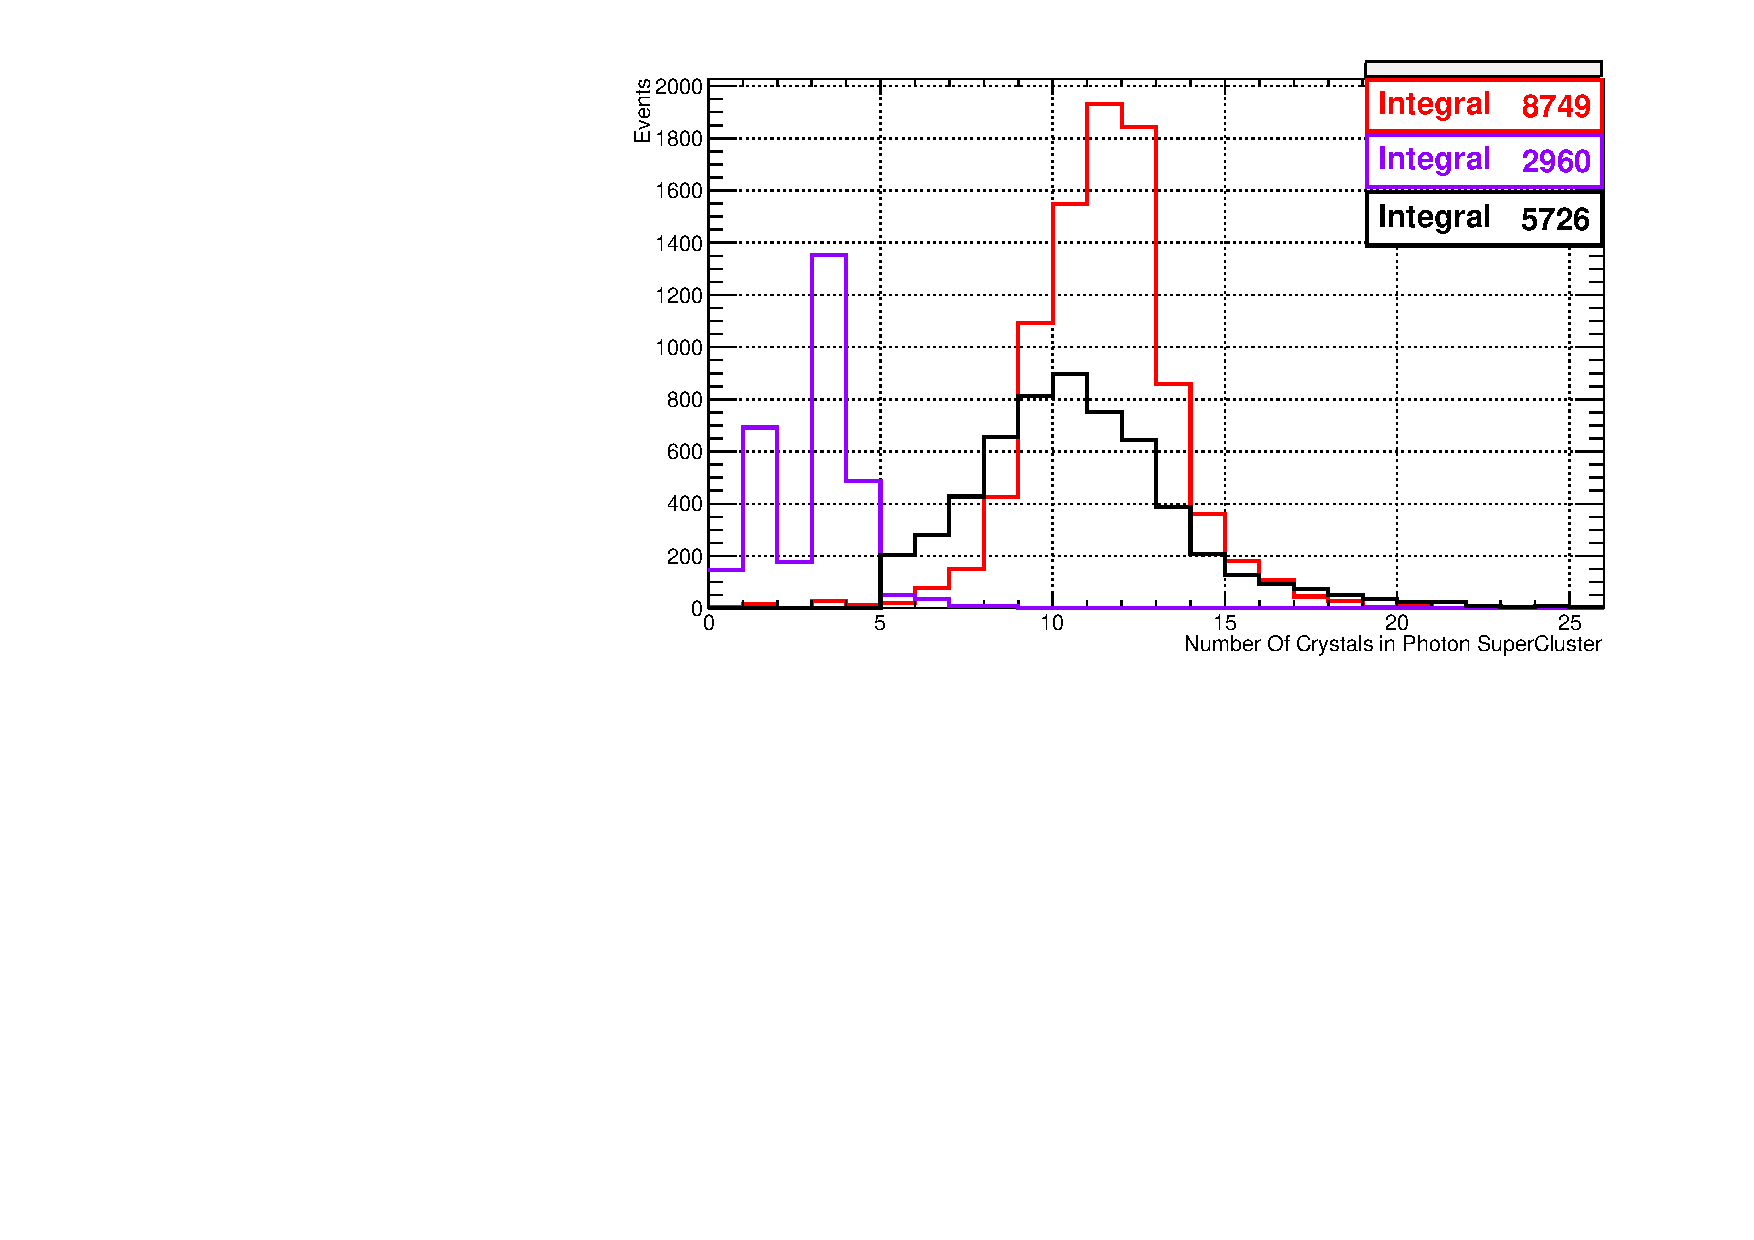
\includegraphics[height=0.50\textwidth, width=0.5\textwidth]{THESISPLOTS/Number-Of-Crystals-In-Photon-SC.pdf}
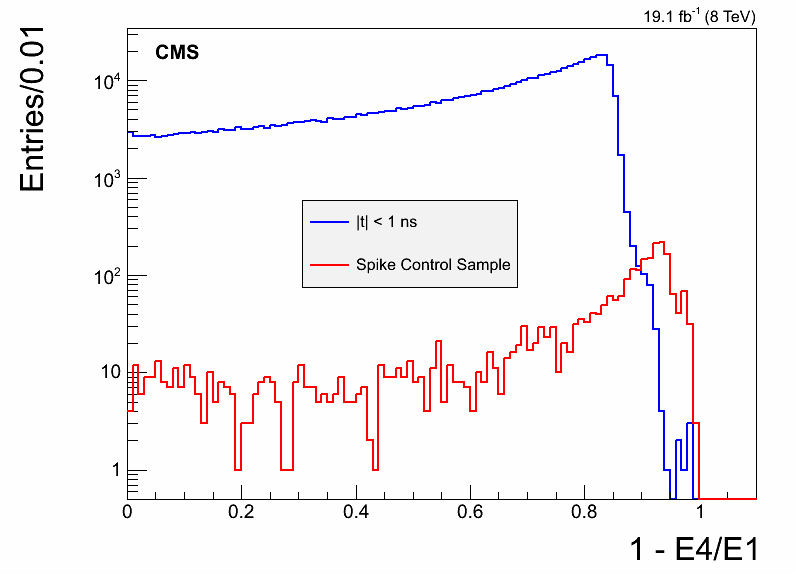
\includegraphics[height=0.50\textwidth, width=0.5\textwidth]{THESISPLOTS/swissX.png} }
\captionof{figure}{\textit{Number of crystals} of a photon supercluster~(left) for in-time photon candidates~(black), spike-seeded photon candidates~(magenta) and halo-induced photon candidates~(red). The spike-seeded photon candidates are selected using a Swiss-Cross variable~($1- E_{4}/E_{1}$)~(right), shown comparing in-time photons~($|t_{\gamma}| < 1.0 $) to spike candidate sample selected using $S_{Minor}$.}
\label{fig:SPIKES}
\end{center}
\end{minipage}

\subsection{Photon Vetoing}
We identify and veto halo-induced, cosmic-induced and spike-seeded photons as follows: 
\begin{itemize}
\item A halo-induced photon is identified and vetoed if a CSC segment for $\rho > 3.32\m$ is found within 0.05 radian of the photon supercluster in $\phi$, \ie a photon with $\Delta\phi(\mbox{CSC Seg},\gamma) < 0.05$ is vetoed. 
%%%%% NOTE %%%%%%%%%%%%%%%%%%%%%%%%%%%%%%%%%%%%%%%%%%%%%%%%%%%%%%%%%%%%%%%%%%%%%%%%%%%%%%%
%%%  |\eta| > 1.6 \equiv \rho > 3.32\m, where \rho = R/sin(\theta) = 1.29\m/sin(2\times actan(e^{-\eta=1.6))
%%%%%%%%%%%%%%%%%%%%%%%%%%%%%%%%%%%%%%%%%%%%%%%%%%%%%%%%%%%%%%%%%%%%%%%%%%%%%%%%%%%%%%%%%%
%We found that we are able to veto events with a  halo photon with 91\% efficiency and 3\% mis-tag rate using this photon selection requirement.
\item A cosmic-induced photon is identified and vetoed if the photon is matched to a DT segment within $\Delta\eta(\mbox{DT Seg},\gamma) < 0.1$, and $\Delta\phi(\mbox{DT Seg},\gamma) < 0.1$. %with $75.5$\% efficiency and $1.4$\% mis-tag rate
\item A spike-seeded photon is vetoed if the photon has an ECAL time $\chi^{2} > 4$, \newline
$\mbox{Number of crystals} < 7$, $ 1-E_{4}/E_{1} > 0.90$ and $S_{Minor} < 0.17$.% with only $0.4$\% mis-tag rate.
\end{itemize}
%Presented in Table \ref{tab:EVTC}, is a summary for the mis-tag rates of the different non-collision background sources. 
%%\begin{minipage}{0.90\linewidth} 
%%\begin{center}
%%\begin{tabular}{|c| c|}
%\mbox{Fake Rate }
%%\hline
%%\bfseries{Background Source} & \bfseries {Fake Rate}(\%)\\
%%\hline\hline
%%\textit{Halo Photons} &  $ < 3$ \\
%%\textit{Cosmic Photons} & $ < 1.4$ \\
%%\textit{Spikes} & $ < 0.4$ \\
%%\hline
%%\end{tabular}
%%\captionof{table}{Fake rates for different non-collision vetoing.}
%%\label{tab:EVTC} 
%%\end{center}
%%\end{minipage}
%%\vspace{5mm}
% and events with $\PW\rightarrow \Pe\Pagne$ decay with the fake photon passing the photon selection requirement.%, recalling that $\vec{{\ETslash}^{\gamma}\hspace{0.15cm}} = \vec{\ETslash\hspace{0.15cm}} + \vec{\pt^{\gamma}}$ adjusting for out-of-time energy deposits not included in the standard missing transverse energy calculations.
% and events with $\PW\rightarrow \Pe\Pagne$ decay to equally have large ${\ETslash}^{\gamma}\hspace{0.15cm}$ and \ETslash\hspace{0.15cm} because of the undetected neutrino.  
\par 
The result of the event tagging is shown in Figure \ref{fig:RESIDUAL}. We observe that most of the non-collision background events are events with halo-induced photons. Very few late arrival time photons are produced from spikes. There is also some significant contribution from cosmic-induced photons. The most interesting observation is the residual out-of-time background~(in red) which could not be tagged. 

\paragraph*{}\mbox{}\\
\begin{minipage}{0.90\linewidth} 
\begin{center}
  \captionsetup{type=figure}
   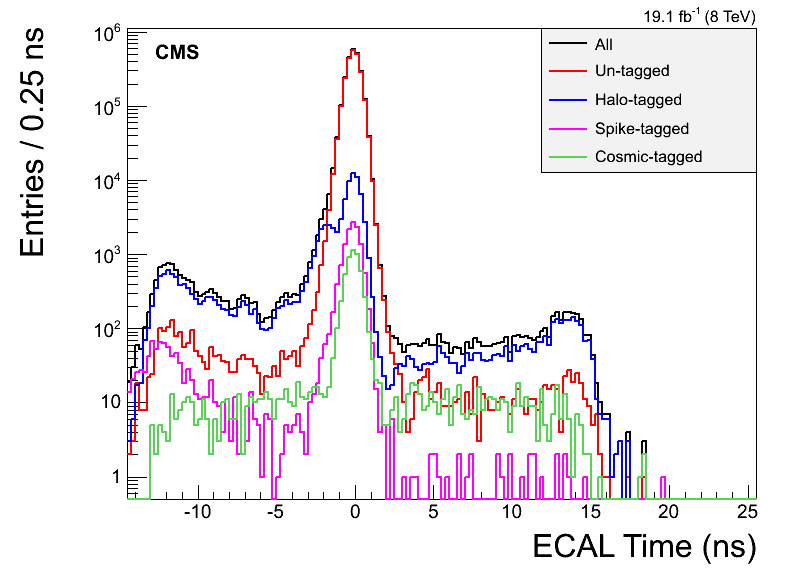
\includegraphics[height=0.7\textwidth, width=0.8\textwidth]{TimeForAll}
%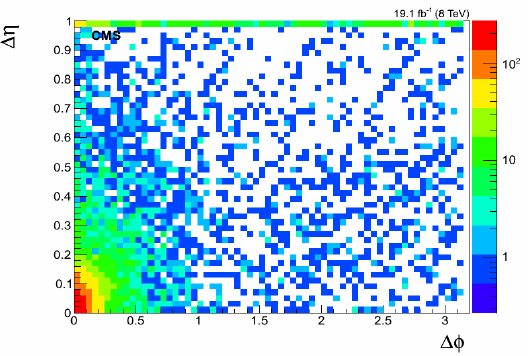
\includegraphics[height=6cm, width=0.5\textwidth]{THESISPLOTS/Cosmic_Ray_Photons_Cosmic_dataset.png} 
   \captionof{figure}{Photon ECAL time, for a data sample of 0 and 1-jet events, showing our tagging performance for non-collision background events.}
   \label{fig:RESIDUAL}
\end{center}
\end{minipage}

\vspace{5mm}

In order to estimate the number of non-collision and collision background events with out-of-time photons contributing to the residual or non-vetoed background photons, we use control samples defined with ${\ETslash}^{\gamma}\hspace{0.15cm}$ and \ETslash\hspace{0.25cm}. We expect the signal events because of the presence of the undetected gravitino to have large~(above 60\GeV) ${\ETslash}^{\gamma}\hspace{0.15cm}$ and \ETslash\hspace{0.15cm}. The non-collision~(cosmic-induced, halo-induced, spike-seeded photons) and collision~(satellite and QCD) background events can be categorized into high transverse momentum~(high-\pt) and low transverse momentum~(low-\pt) photon events.
For high-\pt photon non-collision events, we expect these events to have a large \ETslash\hspace{0.15cm} due to the exclusion of the energy deposits from the photons in the missing transverse energy reconstruction, and small ${\ETslash}^{\gamma}\hspace{0.15cm}$ when the large transverse energy contribution from the energy deposits of the photons is included, while for low-\pt photon non-collision events, we expect these events to have both ${\ETslash}^{\gamma}\hspace{0.15cm}$ and \ETslash\hspace{0.15cm} small since the photon's transverse energy which is excluded is in the first place small. For high-\pt photon collision events which under normal circumstances should have a large missing transverse energy, we expect their \ETslash\hspace{0.25cm} to be large and when the energy deposits from the high-\pt photons is included, we expect their ${\ETslash}^{\gamma}\hspace{0.15cm}$ to be small, while, using the same argument made for low-\pt photon non-collision events, we expect low-\pt collision events to have both small ${\ETslash}^{\gamma}\hspace{0.15cm}$ and \ETslash\hspace{0.15cm}.
A summary of our expectations for ${\ETslash}^{\gamma}\hspace{0.15cm}$ and \ETslash\hspace{0.15cm} for the different expected background events sources with possible contribution to the residual untagged events with out-of-time photon is presented in Table \ref{tab:METSAMPLE}.

\vspace{5mm}
\begin{minipage}{0.90\linewidth} 
  \begin{center}
   \begin{tabular}{c| c|c}
   \toprule
   \hline
     \bfseries{Event Sample} & $\mathbf{\ETslash\hspace{0.15cm}}$ &          $\mathbf{{\ETslash}^{\gamma}\hspace{0.15cm}}$\\
    \hline
    \toprule
   
     Signal Events & Large & Large \\
   %  $\PW\rightarrow \Pe\Pagne$ Events & Large & Large \\
     High-\pt Non-Collision(Mostly Beam Halo) Events & Large & Small \\
     Low-\pt Non-Collision Events & Small & Small \\
     High-\pt Collision(QCD/Ghost) Events & Large & Small \\
     Low-\pt Collision Events & Small & Small \\
     \hline
   \bottomrule     
   \end{tabular}
   \captionof{table}{Summary of missing transverse energy expectation for events with photons.}
   %\caption{\textsf{ABCD} Control samples~(CRs) for estimating non-collision background.}
   \label{tab:METSAMPLE} 
 \end{center}
\end{minipage}

\vspace{5mm}
%Therefore, to minimizing contributions from events anomalous photon time, we restrict our photon arrival time for signal events to within $3.0 < t_{\gamma} < 13.0$~ns, while also requiring that the signal event missing transverse energy be greater than 60\GeV, \ie ${\ETslash}^{\gamma}\hspace{0.15cm} > 60$\GeV, $\ETslash\hspace{0.15cm} > 60$\GeV. This reduces the contribution from ghost/satellite background contributing to the untagged out-of-time photons while at the same time enhances our signal event sample.
%\%clearpage
Using control samples defined using \ETslash\hspace{0.15cm} and ${\ETslash}^{\gamma}\hspace{0.15cm}$ for events with in-time~($|t_{\gamma}| < 2.0$\ns) photons and events with out-of-time~($t_{\gamma} > 3.0$\ns and $t_{\gamma} < -3.0$\ns) photons where each control sample is defined purposely to enhance the contribution of either collision or non-collision background events in the control sample and simultaneously suppressing contributions from the other, we perform a background estimation in the signal sample~($t_{\gamma} > 3.0$\ns, ${\ETslash}^{\gamma}\hspace{0.25cm} > 60$\GeV and $\ETslash\hspace{0.25cm} > 60$\GeV) using the so-called \textsf{ABCD} background estimation method and verify that the background estimation method is performing as expected using a data sample of zero and one jet events where we don't expect any signal events.
% with out-of-time photons, $t_{\gamma} > 3.0$~ns and  ${\ETslash}^{\gamma}\hspace{0.15cm} > 60$\GeV, $\ETslash\hspace{0.15cm} > 60$\GeV  is supposed to be the same if the method is valid. One of our assumption for using the ABCD method is that the background contributions from QCD events and multijets events is negligible. We also study the consequences of this assumption on the number of background estimated events with a separate control sample of mostly out-of-time photon candidates used in reconstructing the true \PZ mass and measure the its candidate electron's arrival time at ECAL since for these events we expect most of the electrons from the $\PZ \rightarrow \EE$ decay to be in-time. Thus, the observed number of out-of-time electron candidates gives us an estimate of the contributions of collision events in our signal sample.

%%\begin{figure}[htbp]
%%  \begin{center}
%%    \captionsetup{type=figure}
%%     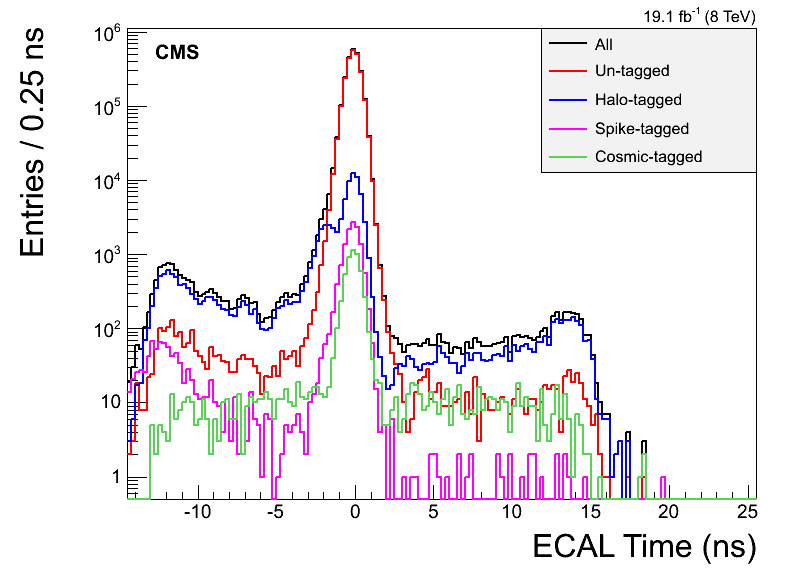
\includegraphics[height=0.7\textwidth, width=0.8\textwidth]{TimeForAll}
%%    \caption{Residual Background(red) after tagging the different non-collision background sources using the selection variables described in text.}
%%    \label{fig:RESIDUAL}
%%   \end{center}
%%\end{figure}
%%\begin{table}[h!]
%% \begin{center}
%%   \begin{tabular}{| l c r |}
%%   \hline
%%   1 & 2 & 3 \\
%%   4 & 5 & 6 \\
%%   7 & 8 & 9 \\
%%   \hline
%%   \end{tabular}
%% \end{center}
%%\caption{A simple table}
%%\end{table}
%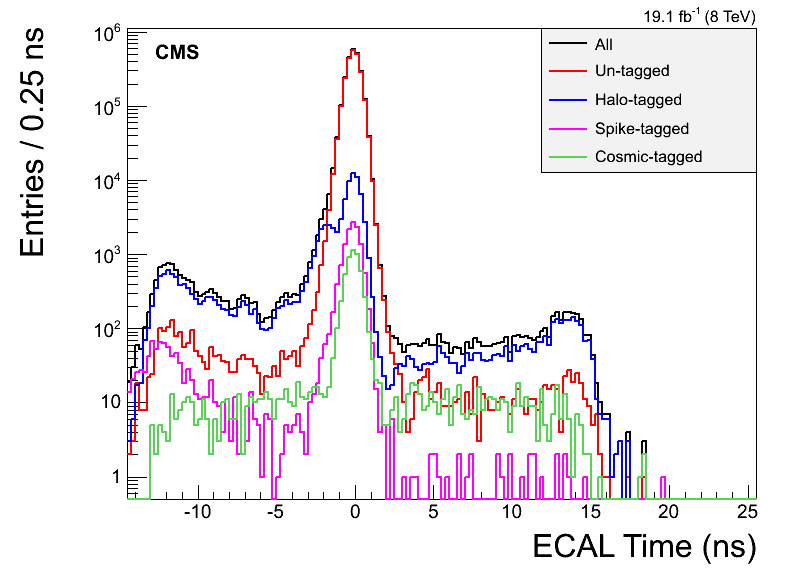
\includegraphics[height=0.7\textwidth, width=0.8\textwidth]{TimeForAll}
%\end{figure}
\subsection{Background Estimation with ABDC Method}
We expect most of the background events to come from non-collision events and so our objective is to estimate the number of non-collision events in the signal control sample using the \textsf{ABCD} technique. We also estimate the possible contamination expected from collision events to these control samples used in the \textsf{ABCD} method.

\subsubsection{Non-Collision Background Estimation}\label{NONBKG}
To estimate the number of background events from non-collision events we define samples labeled as \textsf{ABCD} in photon ECAL time and  $\ETslash\hspace{0.25cm}$ for events selected with ${\ETslash}^{\gamma}\hspace{0.15cm} > 60$\GeV. The events with ${\ETslash}^{\gamma}\hspace{0.25cm} > 60$\GeV define a Control Sample~(CS) where the contribution from collision~(QCD) background events is heavily suppressed as most collision background events have small ${\ETslash}^{\gamma}\hspace{0.15cm}$ mentioned in Table \ref{tab:METSAMPLE}. The samples: \textsf{A} and \textsf{B} shown in Table \ref{tab:NON-COLLISION} contain events with $\ETslash\hspace{0.25cm} < 60$\GeV and $\ETslash\hspace{0.15cm} > 60$\GeV, respectively, and photon ECAL time, $-10.0 < t_{\gamma} < -3.0$\ns, and sample \textsf{C} contain events with $\ETslash\hspace{0.25cm} < 60$\GeV and photon ECAL time, $3.0 < t_{\gamma} < 13.0$\ns.
\newline
The remaining collision-produced background events with some contribution in the \textsf{B} and \textsf{D} samples are estimated in the next section and also corrected for.

\vspace{5mm}
\begin{minipage}{0.90\linewidth} 
  \begin{center}
   \begin{tabular}{|c| c| c|}
   \hline
     \bfseries{Non-Collision} & $\mathbf{\ETslash\hspace{0.25cm}} < 60$\GeV & $\mathbf{\ETslash\hspace{0.25cm}} > 60$\GeV \\     
      \hline \hline
        $3.0 < t_{\gamma} < 13.0$~ns. &  \textsf{$C$} &  \textsf{$D$} \\
      \hline
        $ -10.0 < t_{\gamma} < -3.0$~ns & \textsf{$A$} &  \textsf{$B$} \\
    \hline 
   \end{tabular}
   \captionof{table}{\textsf{Definition of ABCD} samples used for estimating non-collision background events in the signal sample \textsf{D}. Events must satisfy the ${\ETslash}^{\gamma}\hspace{0.15cm} > 60$\GeV selection requirement, which reduces collision background events significantly.}
   %\caption{\textsf{ABCD} Control samples~(CRs) for estimating non-collision background.}
   \label{tab:NON-COLLISION} 
  \end{center}
 \end{minipage}
%%\end{table}
%\begin{itemize}
%\item \textbf{A}: Events with ${\ETslash}$~~$ < 60$~GeV and $ -10.0 < t_{\gamma} < -3.0$~ns.
%\item \textbf{C}: Events with ${\ETslash}$~~$ < 60$~GeV and $3.0 < t_{\gamma} < 13.0$~ns.
%\item \textbf{B}: events with ${\ETslash}$~~$ > 60$~GeV and $-10.0 < t_{\gamma} < -3.0$~ns.
%\item \textbf{D}: events with ${\ETslash}$~~$ > 60$~GeV and $3.0 < t_{\gamma} <  13.0$~ns.
%\end{itemize}

\vspace{5mm}
\par
We assume that the arrival time of a photon is independent of the missing transverse energy in the event and because we are selecting events with out-of-time photons~(where the definition of  $\ETslash\hspace{0.25cm}$ is the same for all events) in defining the \textsf{ABCD} samples, we expect the ratio in the number of events with high-\ETslash\hspace{0.25cm} and low-\ETslash\hspace{0.25cm} for both out-of-time samples to be the same provided the contribution from collision events with mis-measured photon time is not large, \ie $\frac{N_{D}}{N_{C}} = \frac{N_{B}}{N_{A}}$. Thus, the number of non-collision background events with out-of-time photons expected in the signal sample, \textsf{D}, is estimated as
\begin{equation}
N^{non-col}_{D} = \left(\frac{N_{B}}{N_{A}} \right)\cdot N_{C},
\end{equation}
where $N_{B}$ $N_{A}$ and $N_{C}$ are the number of events observed in \textsf{B}, \textsf{A} and \textsf{C} samples in that order and $N^{non-col}_{D}$ is the number of non-collision background events we expect in the signal sample \textsf{D}.
%%%%%
\subsubsection{Collision Background Estimation}
We want to estimate the contribution from collision background events to samples \textsf{B} and \textsf{D} of Table \ref{tab:NON-COLLISION}. Using the \textsf{ABCD} technique once more we define samples in the photon ECAL time and ${\ETslash}^{\gamma}\hspace{0.15cm}$ for events selected with $\ETslash\hspace{0.25cm} > 60$\GeV. The events with $\ETslash\hspace{0.25cm} > 60$\GeV define a control sample where the contribution from collision events is dominant as reflected in Table \ref{tab:METSAMPLE}. Most collision events have in-time~($|t_{\gamma}| < 2$\ns) photons. The few collision events with out-of-time photons which might contribute to \textsf{B} and \textsf{D} samples because the photon time is mis-measured can be estimated using control samples made of in-time photons. The definition of each sample as used in the \textsf{ABCD} method to estimate the out-of-time photon collision background is given in Table \ref{tab:COLLISION}. Samples \textsf{A}, \textsf{B}, \textsf{C},  and \textsf{D} are not the same as samples used in \ref{NONBKG}.

\vspace{5mm}
\begin{minipage}{0.90\linewidth} 
\begin{center}
\begin{tabular}{|c| c| c|}
 \hline
\bfseries{Collision}       & $\mathbf{{\ETslash}^{\gamma}\hspace{0.25cm}} < 60$\GeV &  $\mathbf{{\ETslash}^{\gamma}\hspace{0.25cm}} > 60$\GeV \\      
\hline \hline
$3.0 < t_{\gamma} < 13.0$\ns. &  \textsf{C} &  \textsf{D} \\
\hline
$ -2.0 < t_{\gamma} < 2.0$\ns & \textsf{E} &  \textsf{F} \\
\hline 
$ -10.0 < t_{\gamma} < -3.0$\ns & \textsf{A} &  \textsf{B} \\
\hline
\end{tabular}
\captionof{table}{\textsf{A,B,C,D,E,F} samples used for estimating collision background events with out-of-time photons contamination the samples \textsf{B} and \textsf{D} defined in Table \ref{tab:NON-COLLISION}. Events must satisfy $\ETslash\hspace{0.25cm} > 60$\GeV selection requirement. }
\label{tab:COLLISION} 
\end{center}
\end{minipage}

\vspace{5mm}

Using a similar argument that the photon arrival time is independent of the missing transverse energy,
the number of collision events contributing to the sample \textsf{B}, $N_{B}^{col}$, is estimated as 
\begin{equation}{\label{eq:COLB}}
\displaystyle{N_{B}^{col} = N_{B}  = \left( \frac{F}{E} \right)\cdot N_{A}}, 
\end{equation}
and the number of events contributing to the signal sample \textsf{D}, $N_{D}^{col}$, is estimated as
\begin{equation}{\label{eq:COLD}}
\displaystyle{N_{D}^{col} = N_{D}  = \left( \frac{F}{E} \right)\cdot N_{C}},
\end{equation}
where $N_{i}$ is the number of events in each sample, $i=$ \textsf{A,B,C,D,E,F}.
%where the general assumption is that $\frac{N_{B}}{N_{A}}  = \frac{N_{F}}{N_{E}}$ and  $\frac{N_{D}}{N_{C}}  = \frac{N_{F}}{N_{E}}$, 

%\begin{itemize}
%\item $\mathbf{A}$: Events with ${\ETslash}^{\gamma} < 60$~GeV and $-10.0 < t_{\gamma} < -3.0$~ns.
%\item $\mathbf{B}$: Events with ${\ETslash}^{\gamma} > 60$~GeV and $-10.0 < t_{\gamma} < -3.0$~ns.
%\item $\mathbf{E}$: Events with ${\ETslash}^{\gamma} < 60$~GeV and $|t_{\gamma}| < 2.0$~ns.
%\item $\mathbf{I}$: Events with ${\ETslash}^{\gamma} > 60$~GeV and $|t_{\gamma}| < 2.0$~ns.
%\end{itemize}
%we also define a in time CR as:
%\begin{itemize}
%\item $\mathbf{C}$: Events with ${\ETslash}^{\gamma} < 60$~GeV and $ 3.0 < t_{\gamma} <  13.0$~ns.
% \item $\mathbf{D}$: Events with ${\ETslash}^{\gamma} > 60$~GeV and $3.0 < t_{\gamma} <  13.0$~ns.
% \item $\mathbf{E}$: Events with ${\ETslash}^{\gamma} < 60$~GeV and $|t_{\gamma}| < 2.0$~ns.
%\item $\mathbf{I}$: Events with ${\ETslash}^{\gamma} > 60$~GeV and $|t_{\gamma}| < 2.0$~ns.
%\end{itemize}
\subsubsection{Combined Background Estimation}
Now that we have estimates for both collision and non-collision event contributions we can estimate the total number of background events expected in the signal sample \textsf{D}~(Events with $\ETslash\hspace{0.25cm} > 60$\GeV, ${\ETslash}^{\gamma}\hspace{0.15cm} > 60$\GeV and $3.0 < t_{\gamma} < 13.0$~ns) as
\begin{equation}{\label{eq:FBKG}}
N_{D}^{Total} = \left(\frac{N_{B} - N_{B}^{col} }{N_{A}} \right)\cdot N_{C} + N_{D}^{col} = N_{D}^{non-col} + N_{D}^{col}.
\end{equation}
%%where $N_{D}^{non-col}$ and $N_{D}^{col}$ are the contributions from non-collision and collision background events, respectively. 
%\begin{center}
%\centering
%\mbox{
%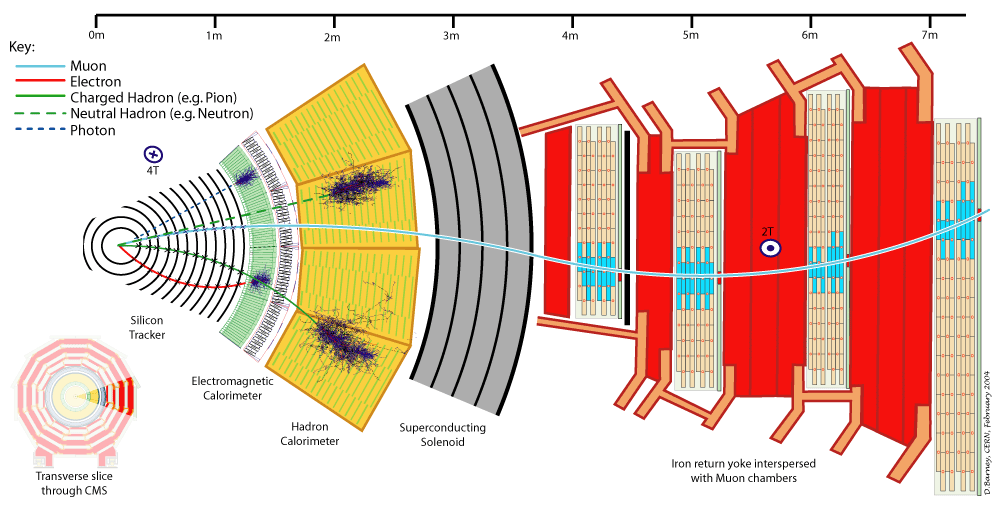
\includegraphics[scale=0.2]{THESISPLOTS/CMS_Slice.png}
%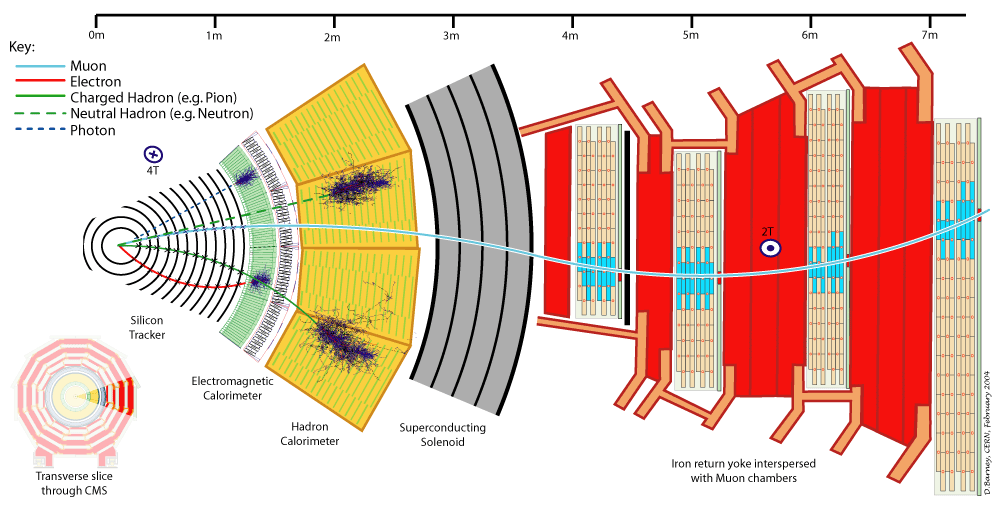
\includegraphics[scale=0.2]{THESISPLOTS/CMS_Slice.png}
%\captionof{figure}{Diagrams showing background estimation technique.}
%\label{fig:BKGESTI}
%\end{center}
\subsubsection{Background Estimation Method Validation}
We verify that our background estimation method performs as expected using a data sample of $0$ and $1$-jet events. We do not expect signal events in this sample.
A statistical agreement between the expected number of background events, obtained using our background estimation method, and the number of events observed in our signal sample \textsf{D}, affirms that the method is reliable. The accepted $0$ and $1$-jet events used must pass the same event selection requirements as potential signal events described in Tables \ref{tab:PhotonSel} and \ref{tab:JetSel}, in addition to vetoing non-collision background events. The event yields in each control sample including tagged events with halo-induced, cosmic-induced and spike-seeded photons is shown in Table \ref{tab:EVTYIELD}.
\newline
Using the event yields in Table \ref{tab:EVTYIELD} for each sample and Equations \ref{eq:COLB} \ref{eq:COLD} and \ref{eq:FBKG} we obtain the following estimates for the expected number of events in signal sample \textsf{D}:
\begin{align*} 
 N_{B}^{col} &= \frac{35271}{1445254} \times 8 = 0.64^{+0.35}_{-0.34} , \\
 N_{D}^{col} &= \frac{35271}{1445254} \times 2 = 0.46^{+0.11}_{-0.09} , \\
 N_{D}^{Total} &= \left( \frac{38 - 0.64}{851}\times 359\right) +  0.46 = 16.41^{+3.00}_{-2.59}.
\end{align*}
The uncertainty are statistical uncertainties based on the event statistics in each sample. Our expected number of background events in signal sample \textsf{D} is $16.41^{+3.00}_{-2.59}$  which is within the statistical uncertainties agreeable with the 10 events we observe in the signal sample \textsf{D}. 
This gives us confidence in our background estimation method and the impetus to use the method in our background estimation for real signal events.
% We observed $10$ events while from using Equation \ref{eq:FBKG}, we expected $16.78^{+2.95}_{-3.45}$. We argue that within our statistical uncertainties, there is quite an agreement between our expectation and observed events. The complete result from our closure test is shown in Table \ref{tab:EVTC}. This gives us confidence that our  background estimation method is robust and reliable. We apply the same \textsf{ABCD} to estimate the background contribution in our signal sample. Our signal sample consist of events with at least $2$-jets, at least a single photon and ${\ETslash}^{\gamma}\hspace{0.15cm} > 60$\GeV, $\ETslash\hspace{0.15cm} > 60$\GeV
%\paragraph*{}\mbox{}\\
%\begin{minipage}{\linewidth} 
%\begin{center}
%\begin{tabular}{|c| c| c|}
%\mbox{Fake Rate }
%\hline
%\bfseries{Non-Collision} &  $\mathbf{{\ETslash}^{\gamma}\hspace{0.15cm}} < 60$\GeV & $\mathbf{{\ETslash}^{\gamma}\hspace{0.15cm}} > 60$\GeV \\
%\hline
% $3.0 < t_{\gamma} < 13.0$~ns & \textsf{C}($405$) & ~\textsf{D}($10$) \textcolor{blue}{16.78} \\
% $-10.0 < t_{\gamma} < -3.0$~ns & \textsf{A}($871$) & ~\textsf{B}($36$) \\
%\hline \hline
%\bfseries{Collision} & $\mathbf{\ETslash\hspace{0.15cm}} < 60$\GeV & $\mathbf{\ETslash\hspace{0.15cm}} %> 60$\GeV \\
%\hline 
% $3.0 < t_{\gamma} < 13.0$~ns & \textsf{$D$}($4$) & ~\textsf{D}($10$) \\
% $-2.0 < t_{\gamma} < 2.0$~ns & \textsf{$F^{\prime}$}($1353685$) & ~\textsf{F}($34543$) \\
% $-10.0 < t_{\gamma} < -3.0$~ns & \textsf{$B$}($5$) & ~\textsf{B}($36$) \\
%\hline 
%\end{tabular}
%\captionof{table}{Result from closure test of background estimation technique using 0 and 1-jet events. Numbers in bracket represent our expected background estimate using \textsf{ABCD} method.}
%\label{tab:EVTC} 
%\end{center}
%\end{minipage}
\subsection{Background Estimation Cross Check}
Another method for estimating the number of background events with out-of-time electromagnetic particles from collision is using $\PZ \rightarrow \EE$ events since we expect the electron candidates from \PZ decay to be in-time because of the prompt decay of \PZ bosons. We use events with electron candidates from a \texttt{SingleElectron}~(single electron accepted events) and \texttt{DoubleElectron}~(double electron accepted events) data samples where the contribution from non-collision events to this sample is almost negligible. These events with \PZ bosons are selected such that the energy deposited by out-of-time electron candidates is included in the electron supercluster. The background events under the \PZ boson mass peak may contain electron candidates from collision with mis-measured ECAL time. The out-of-time electron can be randomly matched with another candidate electron to give a di-electron mass which is of the order of the mass of \PZ boson. These background events also include events with poorly reconstructed out-of-time  energy deposits in ECAL which we need to exclude from our study. 
\newline
In order to reduce possible out-of-time events from beam halo and cosmic events happening simultaneously with true $pp$ collision events we only accept events passing the following event selection requirements: the two electron candidates forming a \PZ boson candidate must each have a $\pt > 30$\GeVc, the di-electron mass, $|m_{\EE} - 91| > 61$\GeVcc, both electrons must be in the barrel, \ie $|\eta_{e^{-}}| < 1.479$ and $ |\eta_{e^{+}}| < 1.479$ and the electron arrival time $\chi^{2}$ must be less than  4. The electron's arrival time is taken to be the seed crystal time and corrected to account for the electron's time of flight, which is different from photons. The chosen seed crystal must satisfy the recommended crystal~(reconstructed hit) cleaning criteria; which requires that the seed crystal is not a spike, is not noisy and has been properly time calibrated.
\newline
From the accepted events with \PZ candidates we define a signal event sample for which the di-electron mass is between 76\GeVcc and 100\GeVcc, \ie $76\GeVcc < |m_{\EE}| < 100$~$GeV/c^{2}$, and a background or sideband event sample where the di-electron mass is either between $50\GeVcc < m_{\EE} < 76$\GeVcc or $100\GeVcc < m_{\EE} < 130$\GeVcc. 
\newline
The di-electron mass~(left plot) and electron arrival time~(right plot) of both electron candidates of the \PZ boson~(signal~(blue)) together with the total \PZ boson candidates is shown in Figure \ref{fig:Zmass}.
 
\vspace{5mm}
\begin{minipage}{0.90\linewidth} 
\begin{center}
\mbox{
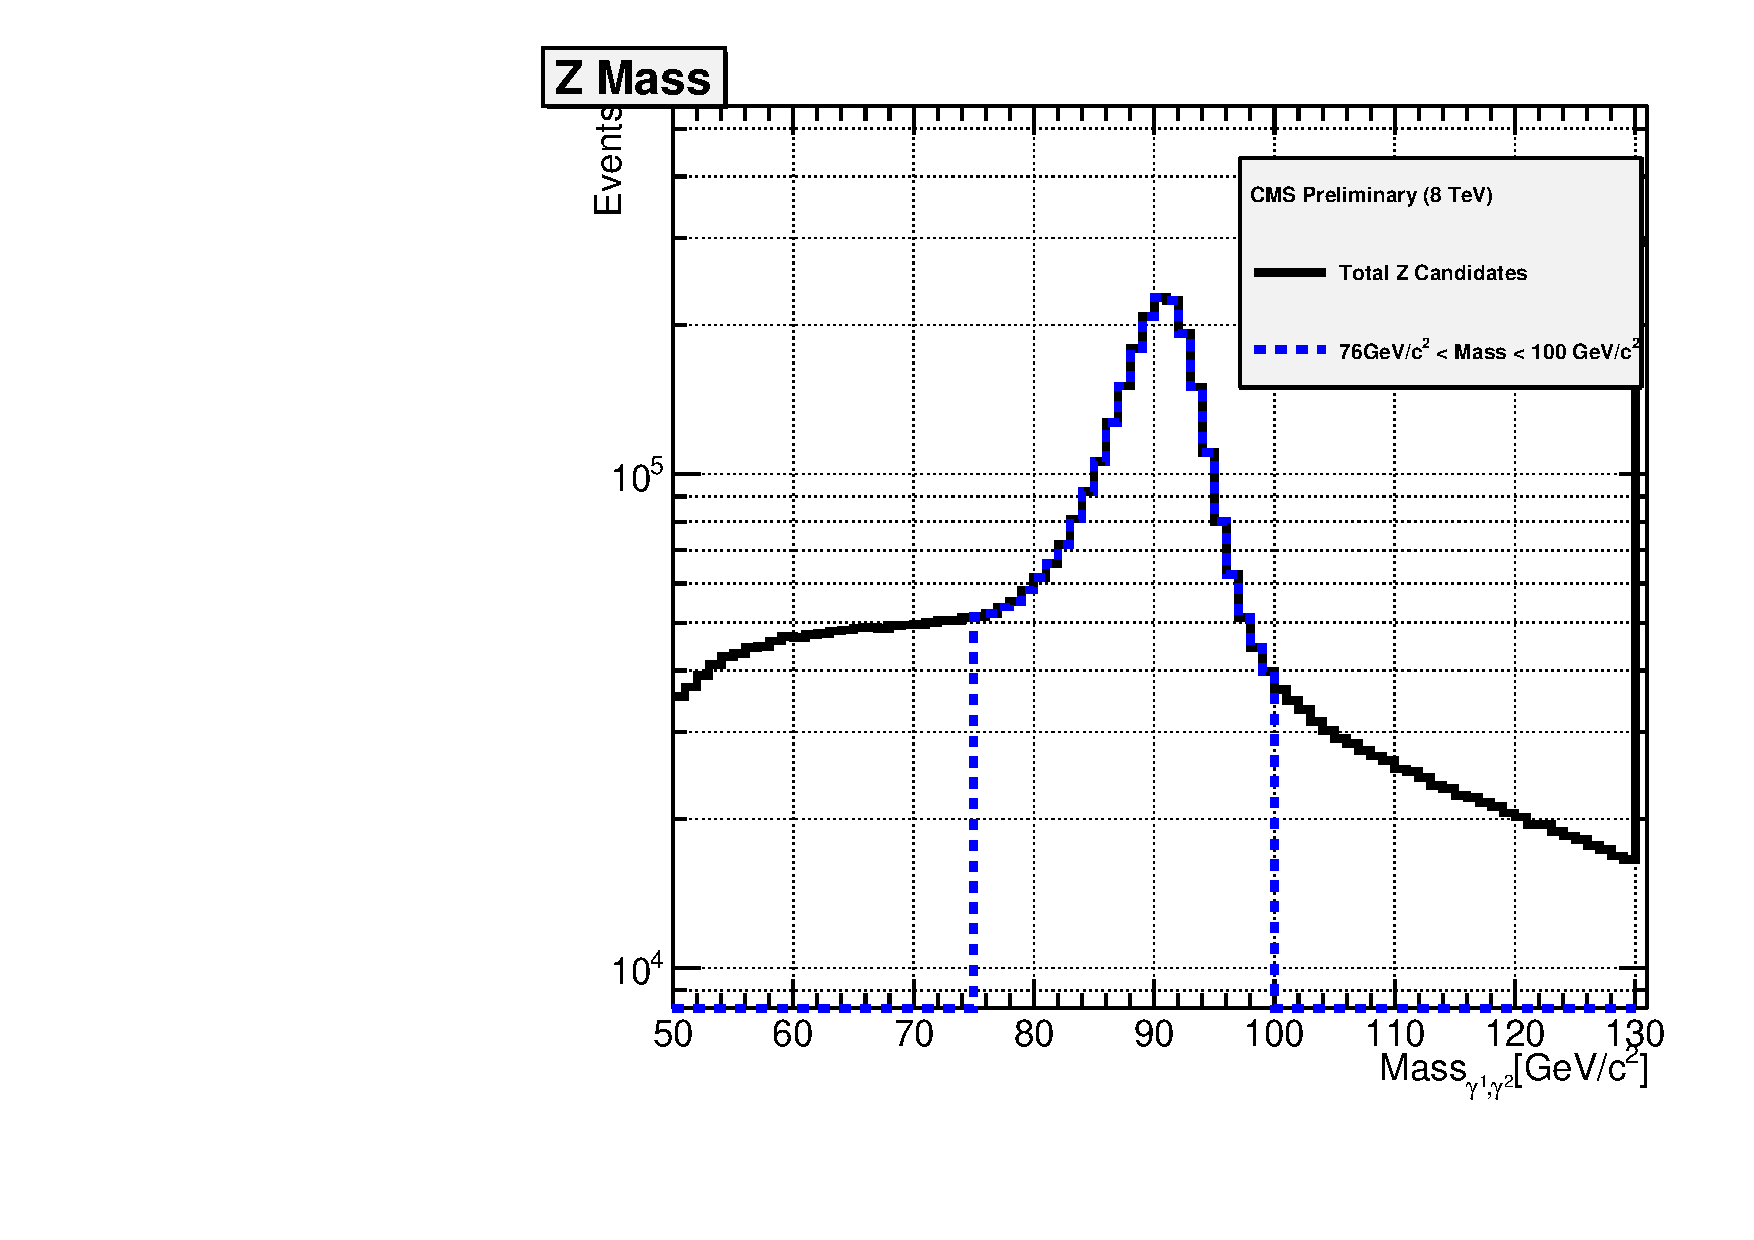
\includegraphics[height=0.55\textwidth, width=0.5\textwidth]{THESISPLOTS/Z-CandidateOverLay-SignalMass.pdf} \quad
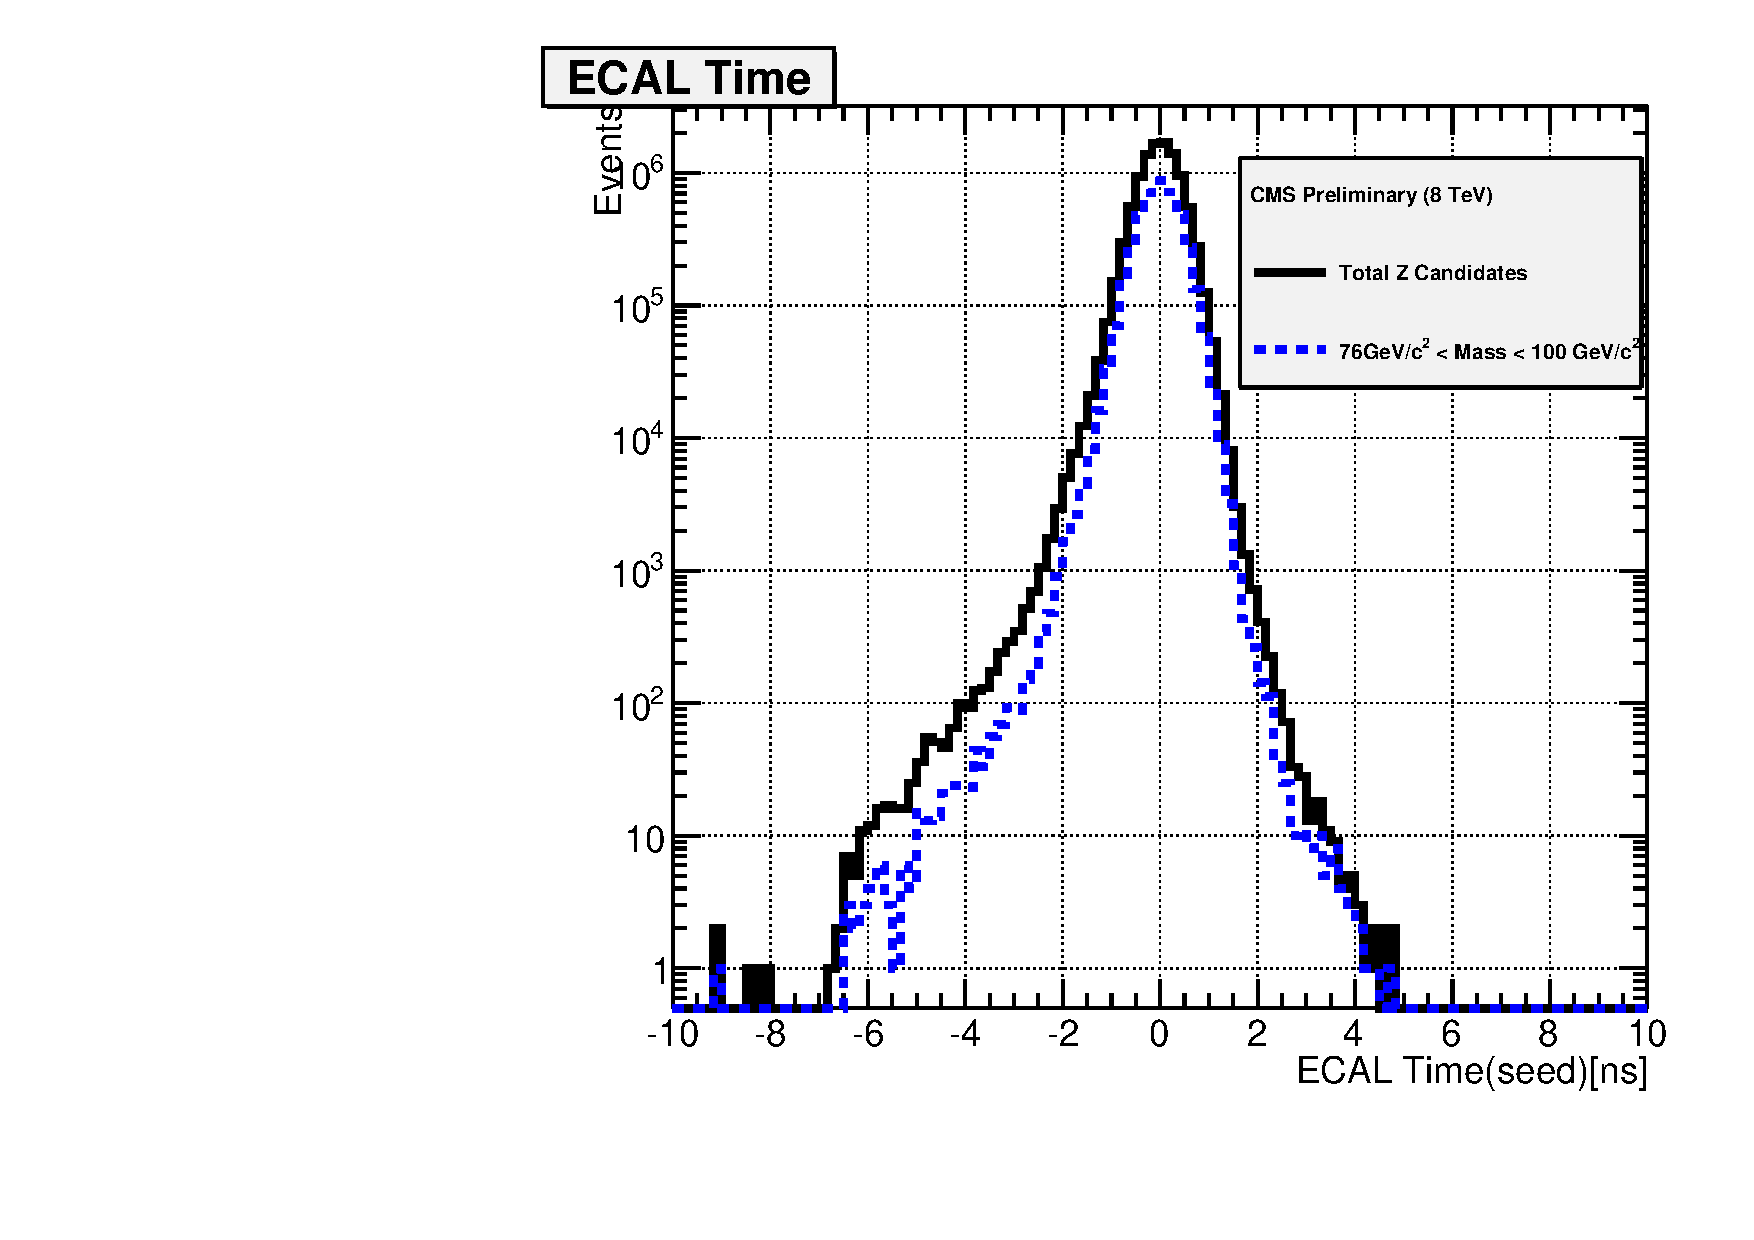
\includegraphics[height=0.55\textwidth, width=0.5\textwidth]{THESISPLOTS/Z-CandidateOverLay-SignalTime.pdf}}
%\mbox{
%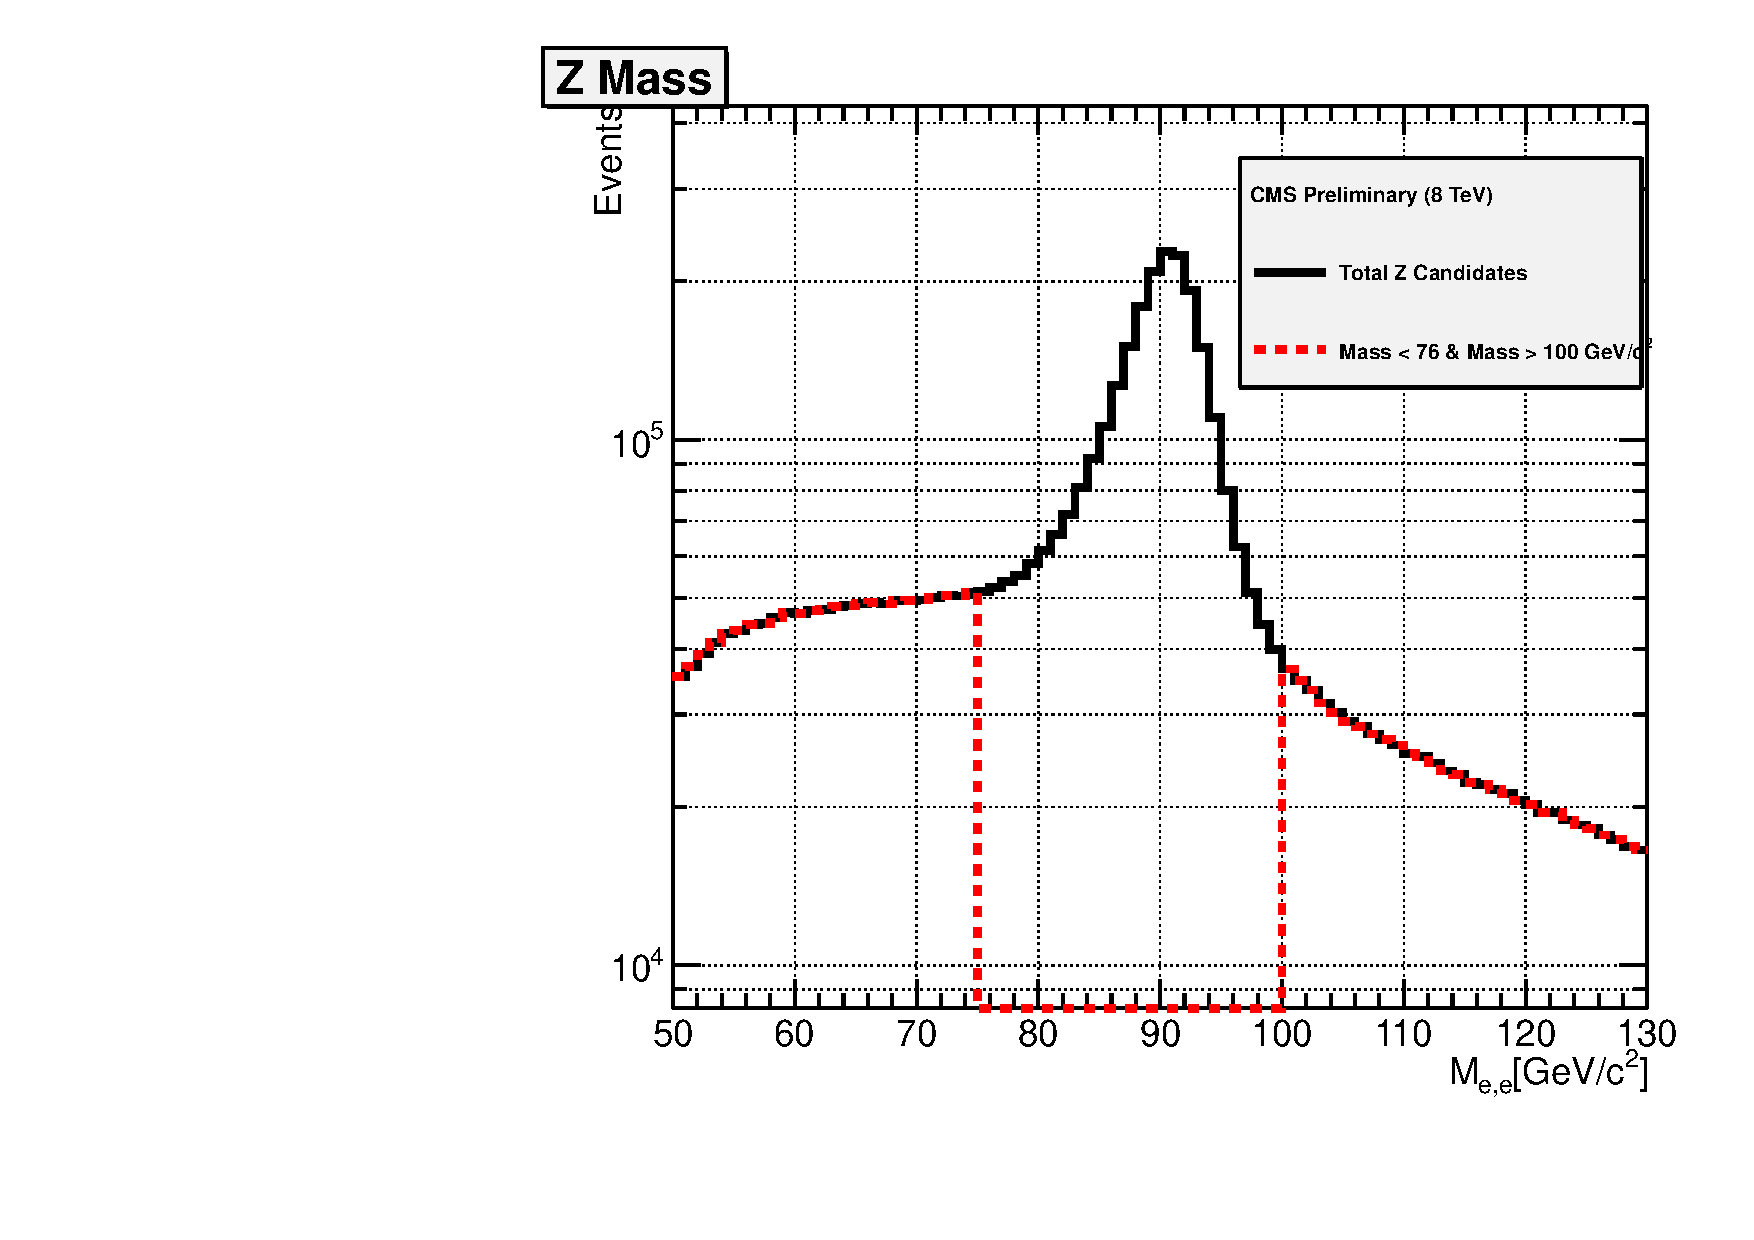
\includegraphics[height=0.55\textwidth, width=0.5\textwidth]{THESISPLOTS/Z-CandidateOverLay-BackgroundMass.pdf}
%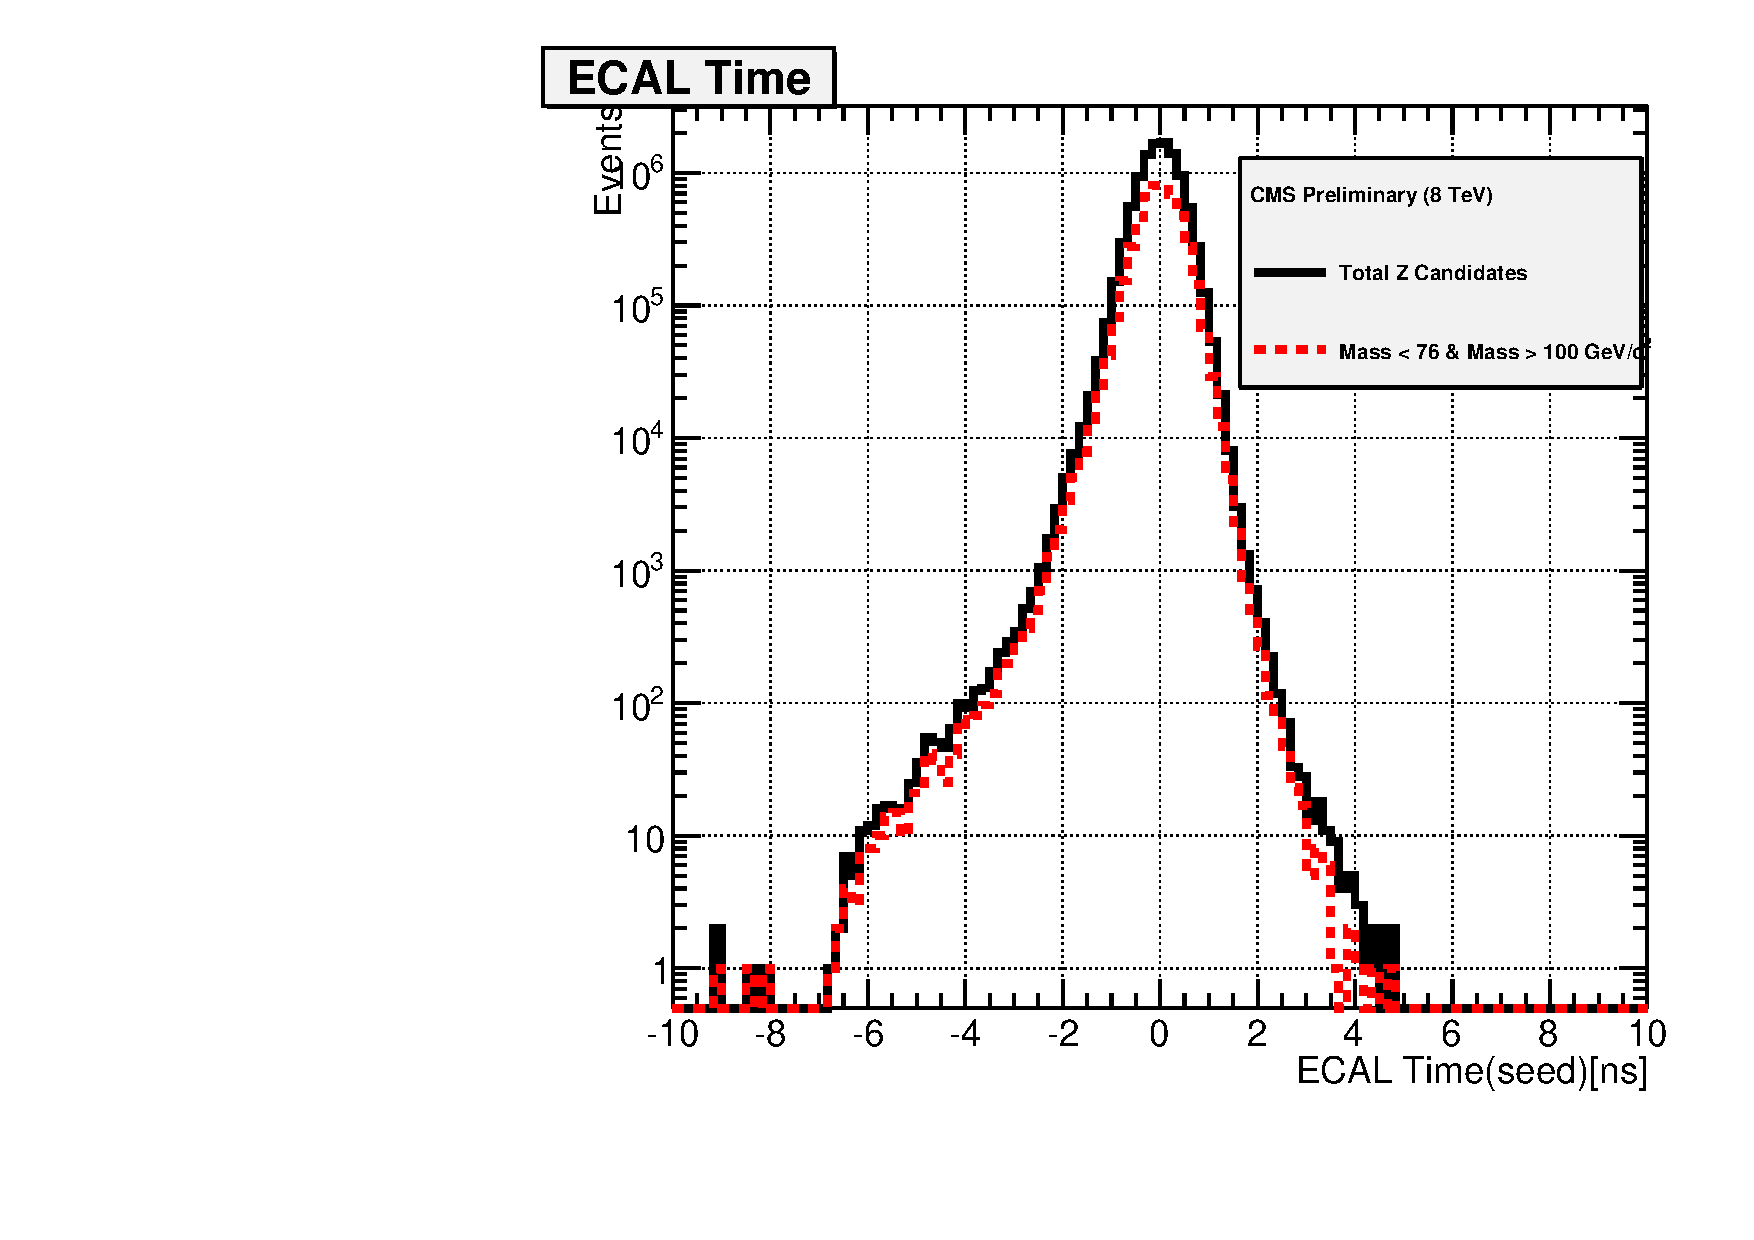
\includegraphics[height=0.55\textwidth, width=0.5\textwidth]{/home/tensr/Documents/TEN-HEP-PHD-THESIS/PHD_THESIS/PHD/THESISPLOTS/Z-CandidateOverLay-BackgroundTime.pdf}}
\captionof{figure}{Di-electron mass distribution~(left) and the time~(right) of the two electron candidates for the signal, $76 < m_{\EE} < 100$\GeVcc, of $\PZ$ boson sample. Events are from the \texttt{Single/DoubleElectron} data sample.}
\label{fig:Zmass}
\end{center}
\end{minipage}

\vspace{5mm}
A scatter plot of the arrival ECAL time against $\eta$~(top right plot) and  $\phi$~(bottom right plots) of both electrons of the \PZ is shown in Figure \ref{fig:Elec}. A clear difference in the scatter plots is seen comparing events from the \texttt{Single/DoubleElectron} data sample~(plots on the right), which do not have the familiar beam halo features~(the "cross-shape" and high event concentration at $\phi = 0,\pm \pi$), to events from \texttt{SinglePhoton} data sample~(plots on the left). 
We conclude that, the candidate \PZ event sample is free from contamination from non-collision events and is useful for estimating out-of-time background events from collisions.

\vspace{5mm}
\begin{minipage}{0.90\linewidth} 
\begin{center}
\mbox{
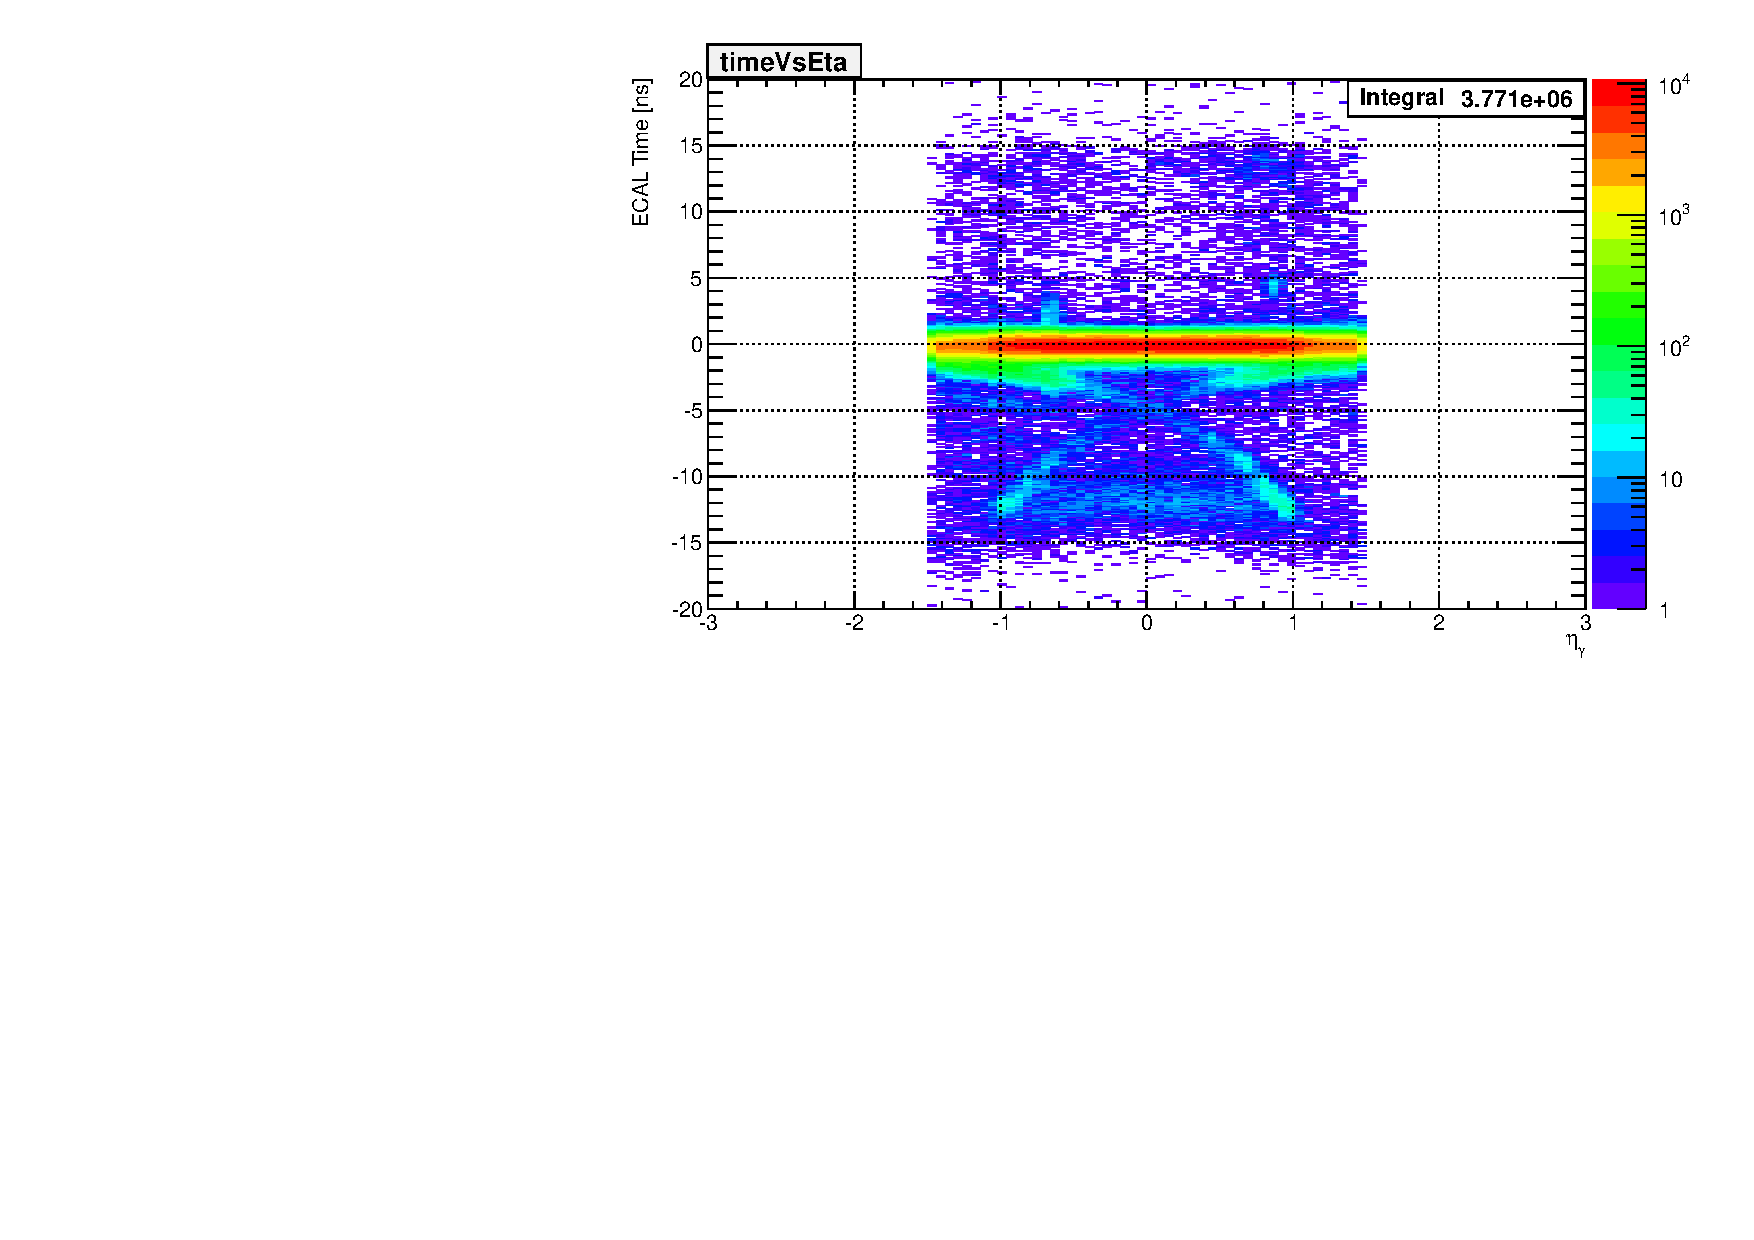
\includegraphics[height=0.50\textwidth, width=0.5\textwidth]{THESISPLOTS/SinglePhotonDataSet-TimeVsEtaEB.pdf}
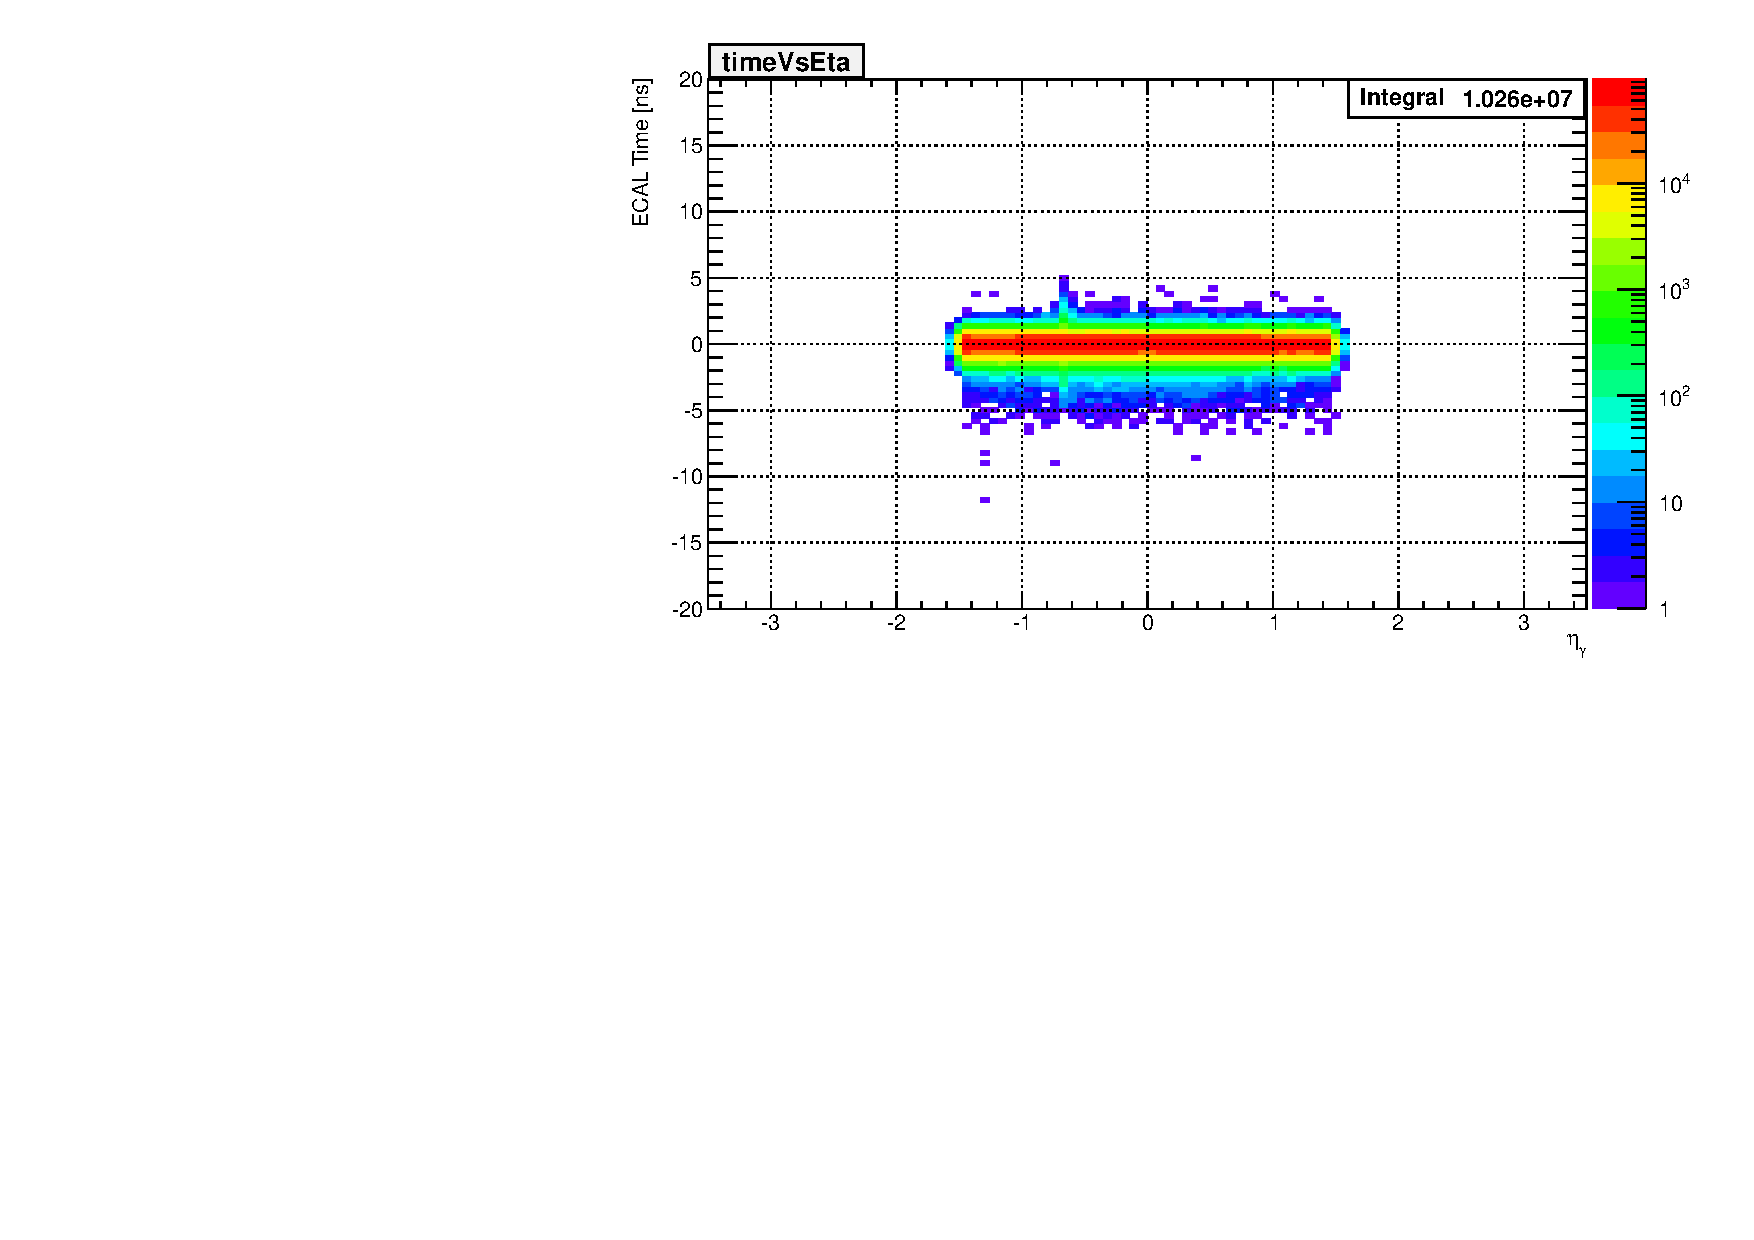
\includegraphics[height=0.50\textwidth, width=0.5\textwidth]
{THESISPLOTS/ZCandidates_TimeVsEta.pdf}}
\mbox{
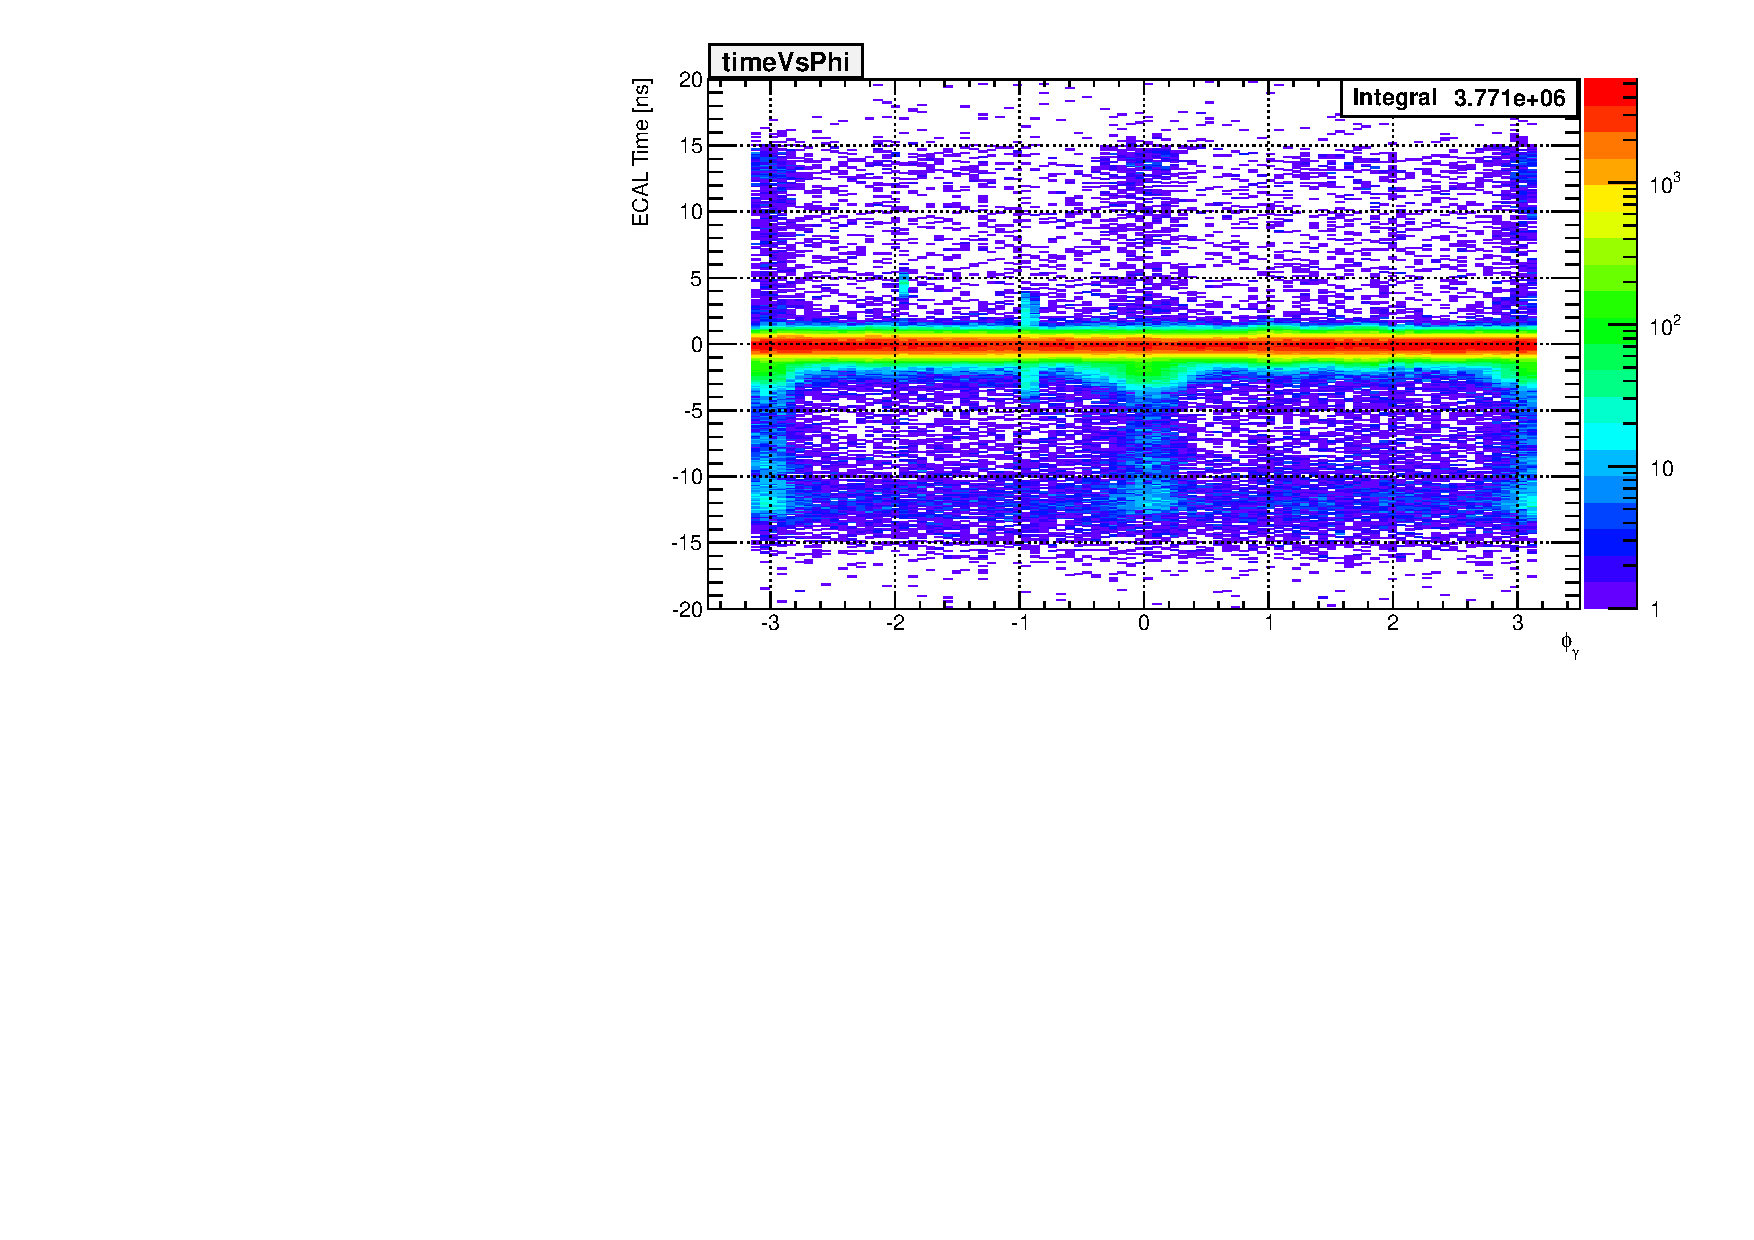
\includegraphics[height=0.50\textwidth, width=0.5\textwidth]{THESISPLOTS/SinglePhotonDataSet-TimeVsPhiEB.pdf}
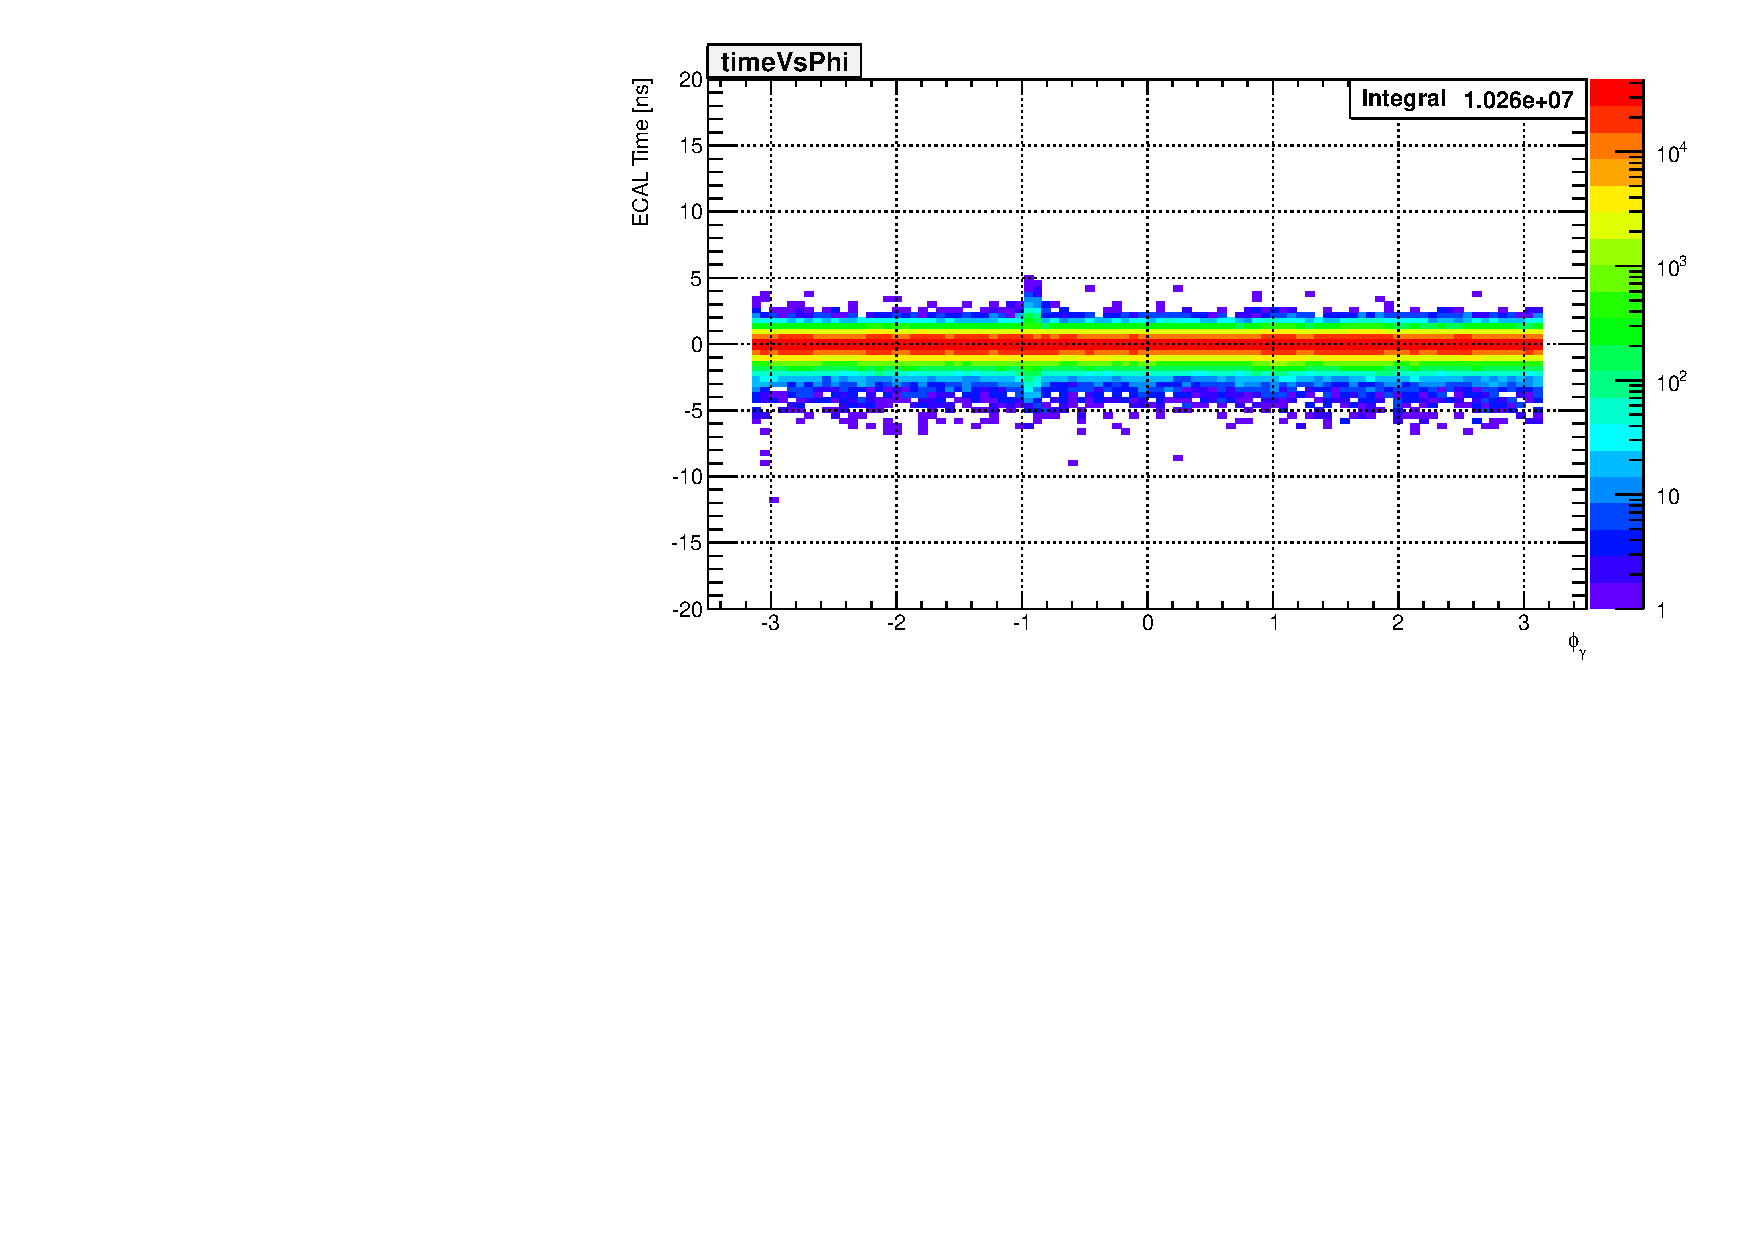
\includegraphics[height=0.50\textwidth, width=0.5\textwidth]{THESISPLOTS/ZCandidates_TimeVsPhi.pdf}}
\captionof{figure}{ECAL time $Vs$ $\eta$~(top plots) and $Vs$ $\phi$~(bottom plots) for electromagnetic particle candidates from \texttt{SinglePhoton} data sample~(left) compared to electromagnetic particle candidates from the \texttt{Single/DoubleElectron} data sample~(right). All electromagnetic particle candidates are in barrel. Most of the electromagnetic particles with "cross-shape" and at $\phi = 0, \pm \pi$, are halo-induced photons.}
\label{fig:Elec}
\end{center}
\end{minipage}

\vspace{5mm}
\par
In order to estimate the out-of-time background events from collision we need the probability for an in-time~($|t| < 2$\ns) event to become out-of-time~($t < -3$\ns or $t > 3$\ns) because of the mis-measurement of the time of the electron candidates. 
\newline
We estimate this probability by dividing the \PZ candidate events according to their arrival time as follows:
\begin{itemize}
\item In-time \PZ boson events: Both electrons of the \PZ boson candidate have arrival time, $|t| < 2$~ns. Their di-electron mass is shown on the top right plot of Figure \ref{fig:collZ},
\item Early time \PZ boson events: Both electrons of the \PZ boson candidate have arrival time, $t < -3$~ns. Di-electron mass shown in the bottom left plot of Figure \ref{fig:collZ},
\item Late time \PZ boson events: At least one of the electrons of the \PZ boson candidate have arrival time, $t > 3$~ns. The di-electron mass is shown in the bottom right plot of Figure \ref{fig:collZ}.
\end{itemize}

The true \PZ boson events in each of the three \PZ boson event samples defined above is estimated as follows: we first fit, with a polynomial function, a sideband~($50 < m_{\EE} < 76$\GeVcc and $ 100 < m_{\EE} < 130$\GeVcc) of the di-electron mass distribution~(see top left plot of Figure \ref{fig:collZ}). Using the side band fit function, we subtract the integral of the fit function from the total number of \PZ boson candidates in the \PZ boson mass peak~( $76 < m_{\EE} < 100$\GeVcc) in each of the three samples. The result of the subtraction gives an estimate of the true \PZ boson events in the in-time and out-of-time \PZ boson event samples. Table \ref{tab:ZEVENTS} show the resulting number of \PZ boson events.

\vspace{5mm}
\begin{minipage}{0.90\linewidth} 
\begin{center}
\begin{tabular}{c| c| c| c }
\toprule
 \hline
\bfseries{Event Sample}  & \bfseries{Early Time} & \bfseries{In-time} & \bfseries{Late Time}   \\
        &  ($t < -3$\ns) & ($ |t| < 2$\ns) &  ($t > 3$\ns) \\
\hline
 Total  & 378 & 2349187.0 & 41.0 \\ 
Estimated \PZ boson Background & $329\pm 0.055 $  & 996803.6  & $8.6\pm 0.341$ \\
Estimated signal \PZ bosons   & $49\pm 0.020 $ & 1352383.4  &  $32.4\pm 0.176$ \\
\hline
\bottomrule
\end{tabular}
\captionof{table}{Number of \PZ boson events with di-electron invariant mass,  $76 < m_{\EE} < 100$\GeVcc) in the in-time and out-of-time \PZ boson samples.}
\label{tab:ZEVENTS} 
\end{center}
\end{minipage}

\vspace{5mm}
The 32.4 events for the late time \PZ boson events consist of 3 \PZ events with both electrons with time, $t > 3$\ns. These 3 \PZ events could be attributed as produced from satellite bunch collisions since the ratio of these 3 events to in-time \PZ events~(1.35 million) from main proton bunch collisions is of the order $10^{-6}$ which is consistent with the expected luminosity at collision for satellite bunches. The intensity of satellite proton bunch is about $10^{3}$ less than that for the main proton bunches \cite{ATLAS-GHOST,CMS-GHOST}. 
\newline
The probability for in-time events producing out-of-time photon candidates, $P_{1}$ is given by $29.4/1352383.4 = 1.09^{+0.28}_{-0.23} \times 10^{-5}$, while the ratio for out-of-time satellite bunch collisions relative to the in-time collision, $P_{2}$, is given by $3/1352383.4 = 2.22^{+1.7}_{-0.96}\times 10^{-6}$. 
\newline
Using this probability and ratio we can predict the number of collision background events in our analysis which have late time~($t > 3.0$) as
\begin{equation}
  N = n_{1} \times P_{1} + n_{2} \times (2P_{1}(1 - P_{1}) + P_{1}^{2}) + n_{1} \times P_{2} + n_{2} \times P_{2}
\end{equation}
where $n_{1}$ is the number of in-time one photon events~(28208) and $n_{2}$ is the number of two photon in-time events~(38) taken from the \textsf{F} sample of the final results of our background estimation presented in Table \ref{tab:EVTYIELD}. 
\par
The estimated the number of background events from collisions in the signal sample \textsf{D}, $N^{col}_{D} = 0.370^{+0.092}_{-0.072}$, events. Comparing this to the estimated background from collision, using the \textsf{ABCD} method, which is $28283/1446522 = 0.093^{+0.093}_{-0.047}$, events, we find that the two methods of estimating the number of background events from collision are not exactly equal. 
However, both method agree that the background contribution from collision events with out-of-time electromagnetic particles is almost negligible~(less than a single event) such that the uncertainties on the ratio of out-of-time to in-time events used in our \textsf{ABCD} collision background estimation does not affect the final results.
%%The out-of-time background contribution to the true \PZ events sample is estimated using a \textit{sideband subtraction method} described as follows:
%%\begin{itemize}
%%\item We fit the di-electron candidate mass distribution of the sideband control sample with a polynomial function(see top plots of Figure  \ref{fig:collZ}) to extract the background template.
%%\item Using the background template, we obtain a scale factor as 
%%\begin{equation}
%%\mbox{Scale Factor} = \frac{N}{M_{1} + M_{2}},
%%\end{equation}
%%shown in the bottom plot of Figure \ref{fig:collZ}, which we used to determine the correct contribution of the background events to the signal event sample.
%%\item After scaling the electrons arrival ECAL time distribution~(red distribution on the bottom right plot in Figure \ref{fig:Zmass}) of the sideband control sample using the extracted scale factor, we subtract the scaled time distribution from the time distribution~(blue distribution of right plot in Figure \ref{fig:Zmass}) of \PZ electron candidates from the signal sample. The resulting ECAL time distribution, shown in Figure \ref{fig:Ztime} is the time distribution from true \PZ events. This ECAL time distribution is used to estimate the number of events with out-of-time electromagnetic particles from collision.
%%\item The ratio of the total number of events with the electron ECAL time, $t > 3$~ns, to those with electron ECAL time, $|t| < 2$~ns, \ie $ N_{t > 3~ns}/ N_{|t| < 2.0~ns}$, gives an estimate of the fraction of out-of-time background events from collision. 
%%\end{itemize}  

\vspace{5mm}
\begin{minipage}{0.95\linewidth} 
\begin{center}
\mbox{
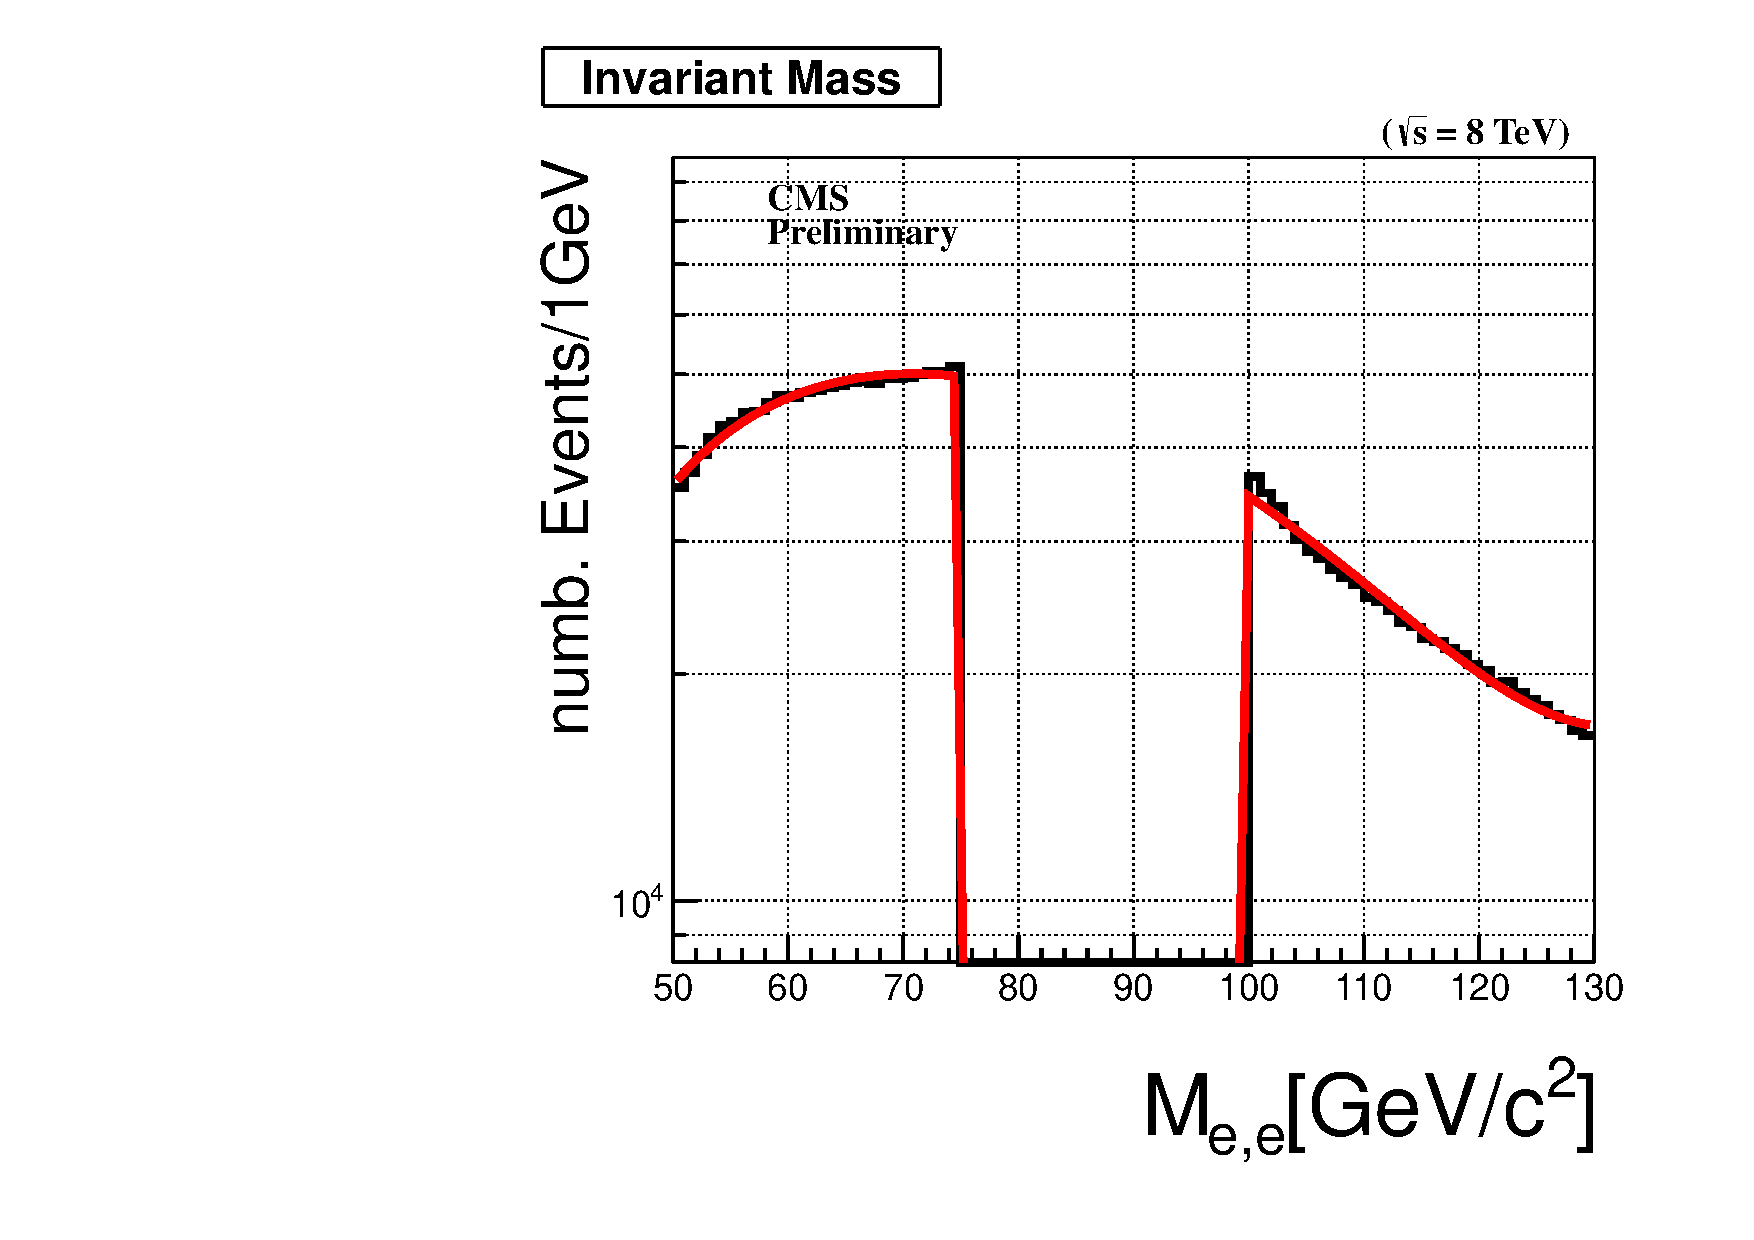
\includegraphics[height=0.550\textwidth, width=0.52\textwidth]{THESISPLOTS/Uncleaned-di-Photon-ZMass-Fit-DoubleElectron-Run2012A.pdf} \quad
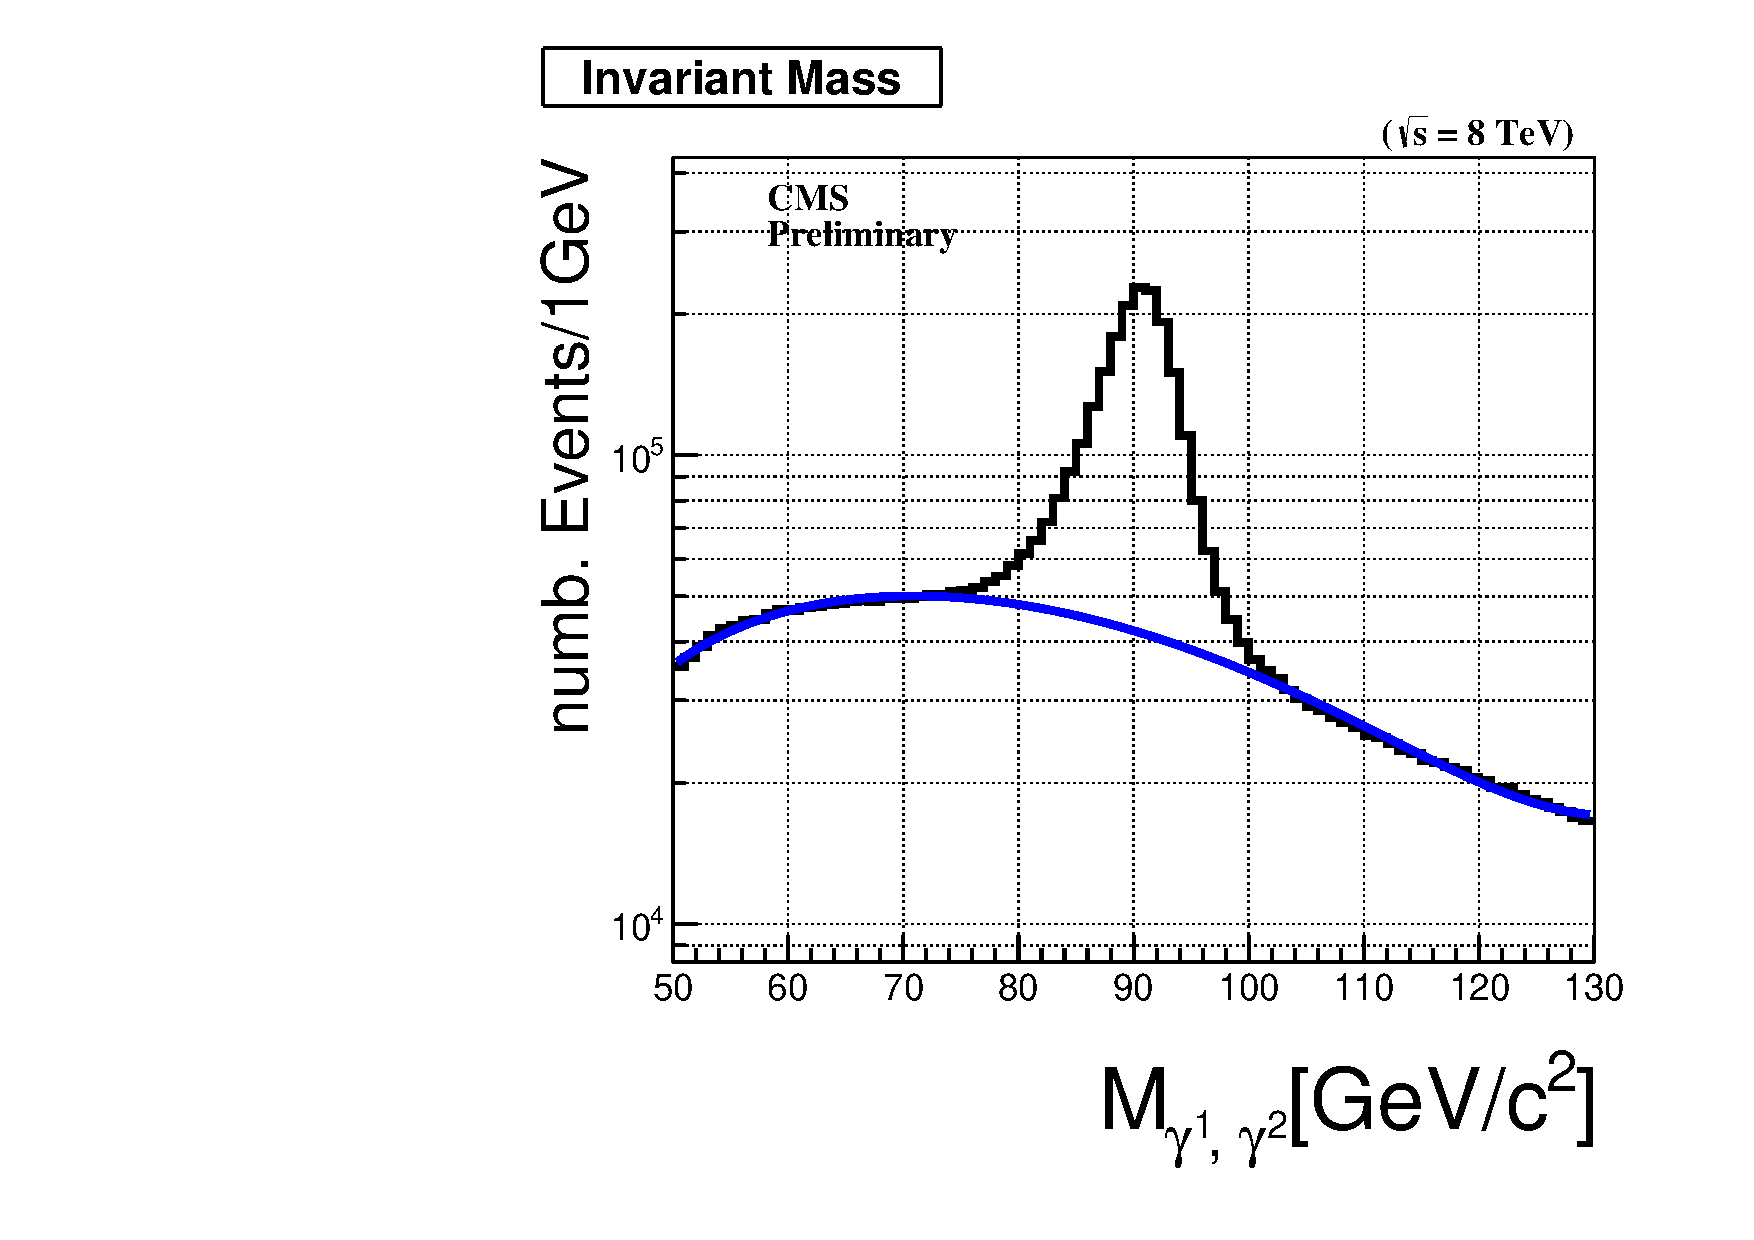
\includegraphics[height=0.550\textwidth, width=0.52\textwidth]{THESISPLOTS/Background_In_ZMass-From-Di-Photon.pdf}
}
\mbox{
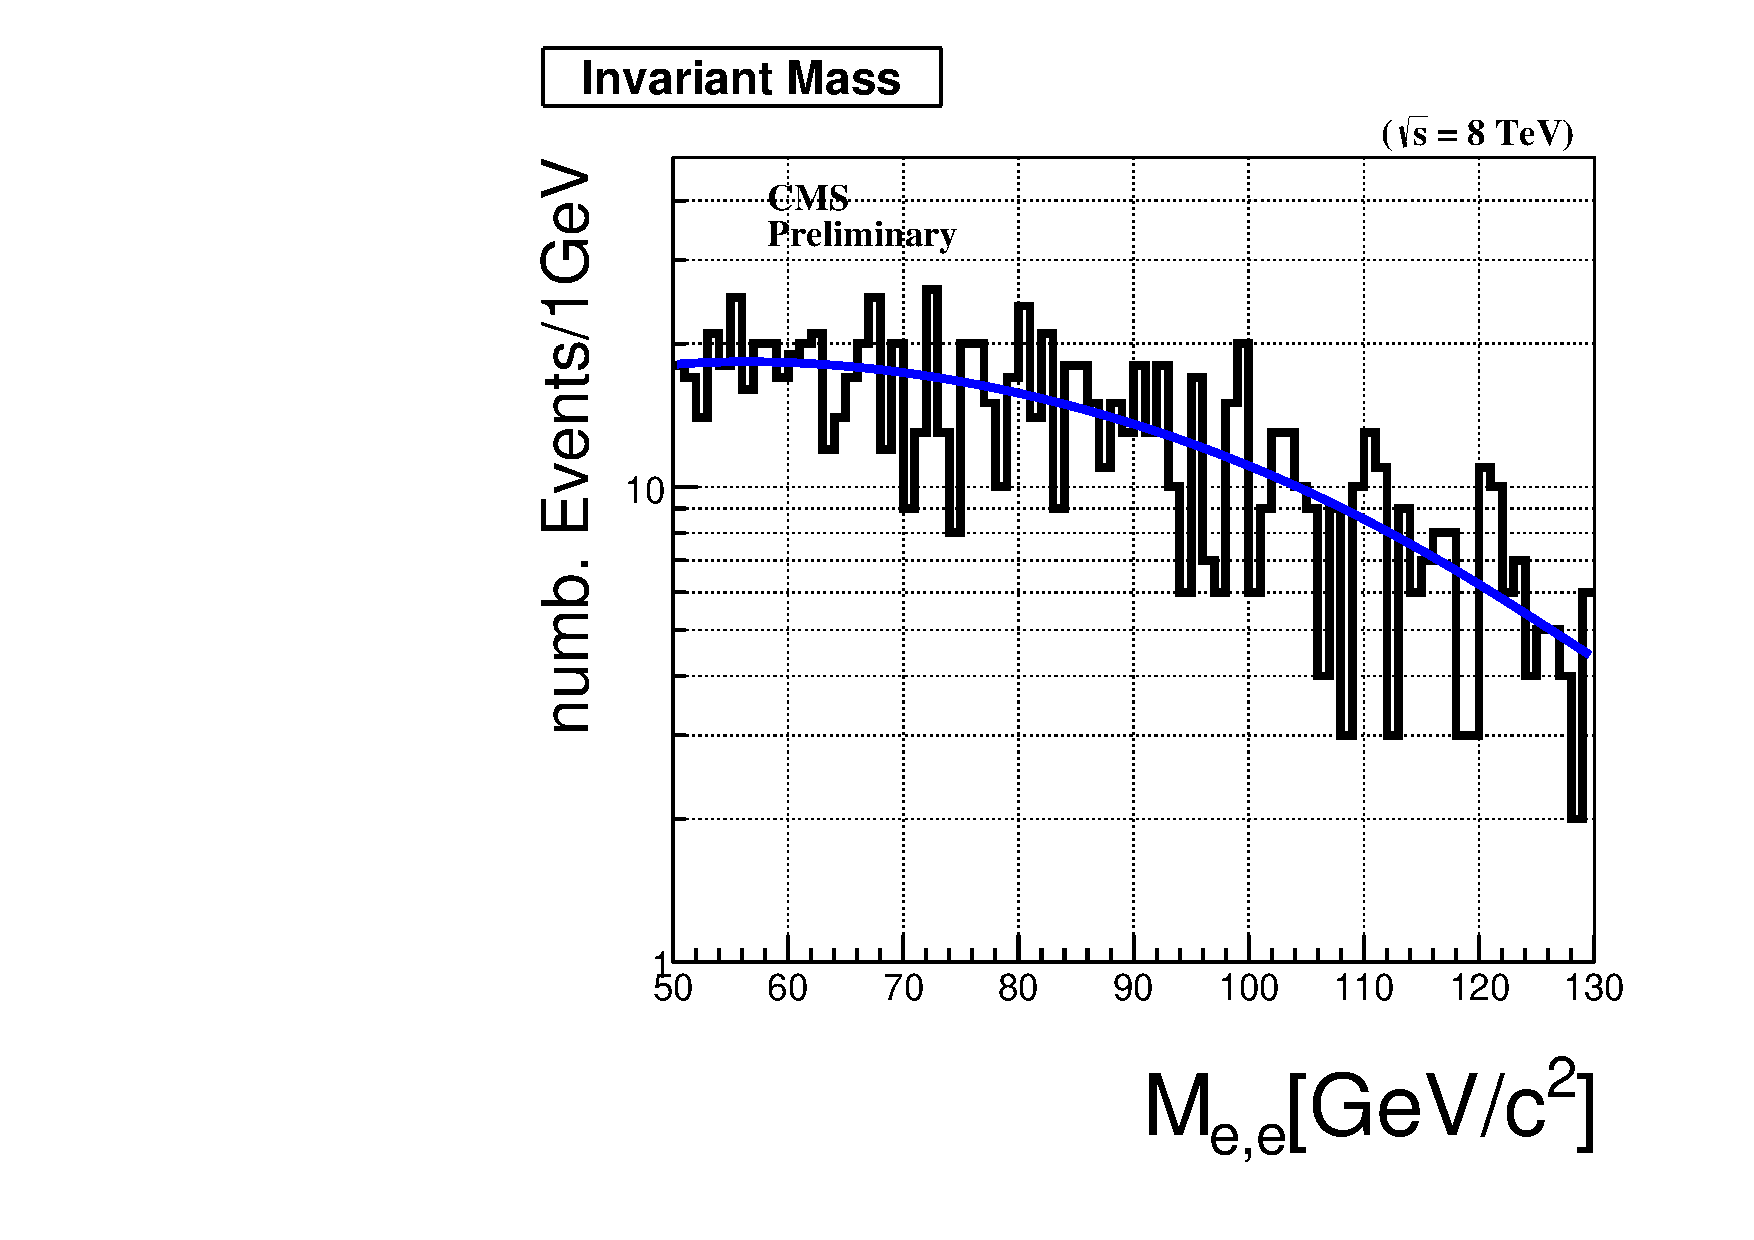
\includegraphics[height=0.550\textwidth, width=0.52\textwidth]{THESISPLOTS/Early-Time-Z-Events.pdf} \quad
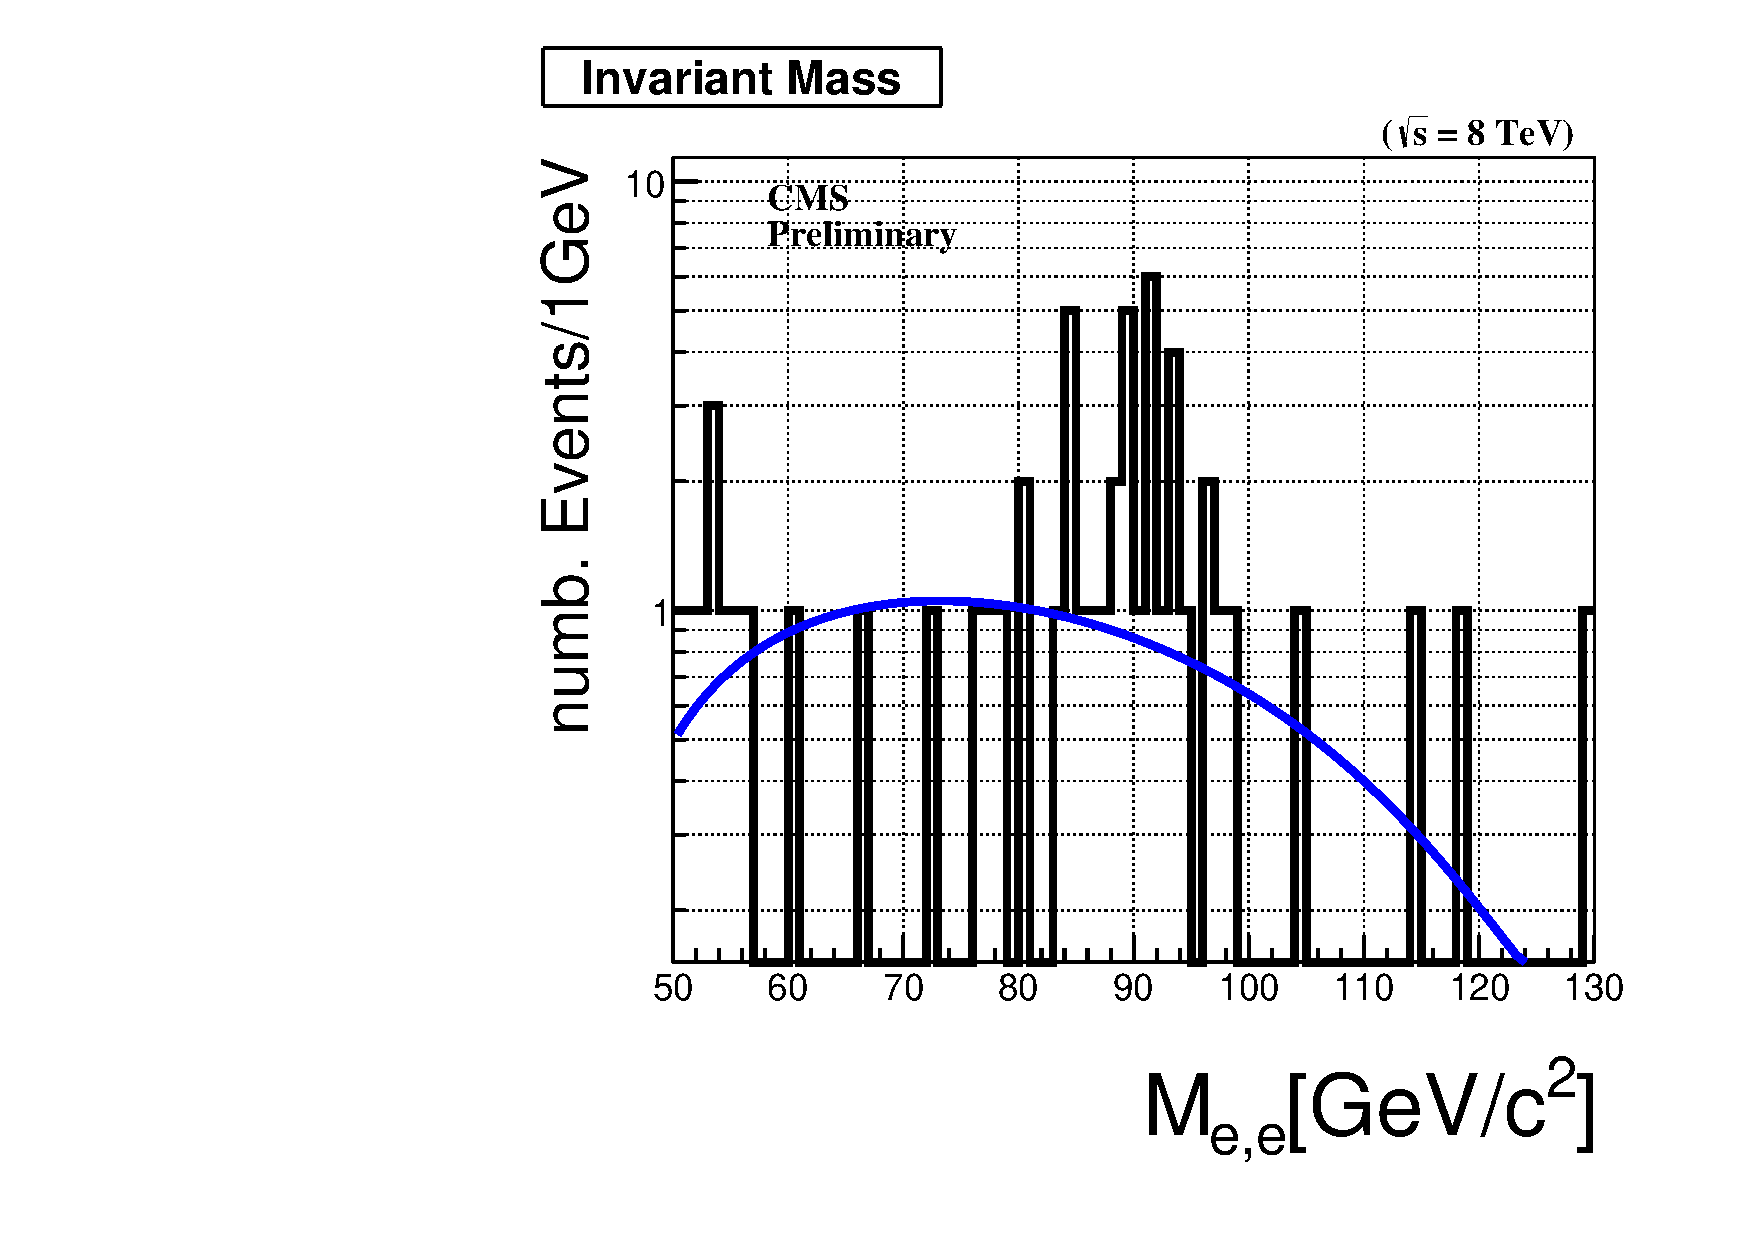
\includegraphics[height=0.550\textwidth, width=0.52\textwidth]{THESISPLOTS/Late-Time-Z-Events.pdf}
%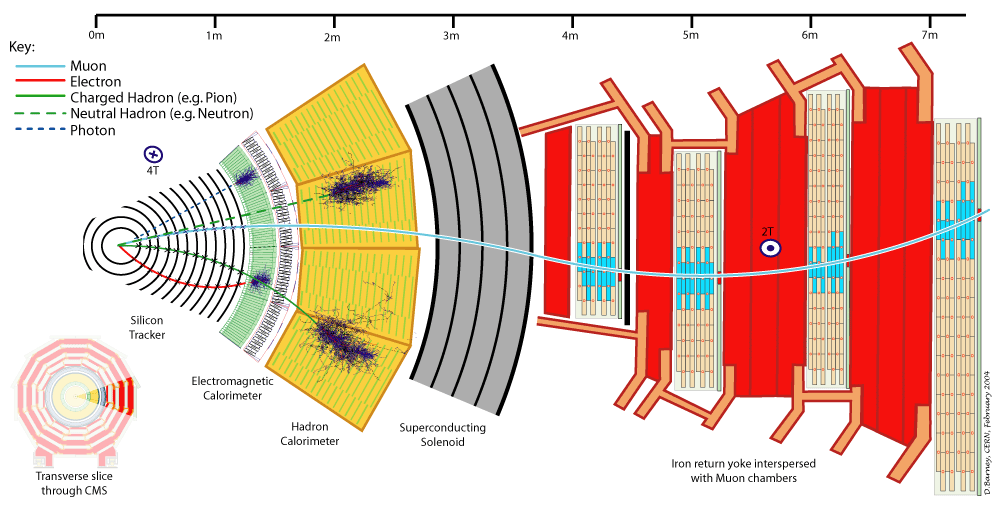
\includegraphics[height=6cm, width=0.5\textwidth]{THESISPLOTS/CMS_Slice.png}
}
\captionof{figure}{
Di-electron invariant mass and polynomial fit~(red) for sideband sample~($50 < m_{\EE} < 76$\GeVcc and $ 100 < m_{\EE} < 130$\GeVcc). Di-electron invariant mass and polynomial fit~(blue) for in-time~($|t| < 2$\ns) \PZ candidates~(\textit{top right}). Di-election invariant mass and polynomial fit for out-of-time~($t < -3$\ns) \PZ candidates~(\textit{bottom left}). Di-election invariant mass and polynomial fit for out-of-time~($t > 3$\ns) \PZ candidates~(\textit{bottom right}). The fits are used to estimated the number of true \PZ bosons in the int-time and out-of-time \PZ candidate samples.}
\label{fig:collZ}
\end{center}
\end{minipage}

\clearpage


%  The estimated ratio for out-of-time events to in-time collision events for the final time distribution of signal electron candidates after the normalized sideband subtraction, shown in Figure \ref{fig:Ztime} is about, $N_{t > 3~ns}/ N_{|t| < 2.0~ns} = 1.29 ^{+0.374}_{-0.325} \times 10^{-5}$.
%\par
%We cannot interpret this inequality  as a disagreement between both methods for estimating the number of background events from collision. On the contrary, this non-agreement can be explained. We have not applied any \MET selection requirements for the \PZ candidate events selection. A simple cut in missing transverse energy, $\MET > 60$\GeV, could further reduce the estimated ratio, $N_{t > 3~ns}/ N_{|t| < 2.0~ns}$, to a very smaller number than what we got. In fact, the smallness of this ratio confirms our speculation that indeed . This means, the number $N^{col}_{D} = 0.366^{+0.106}_{-0.092}$, can be used for our estimated number of background events from collision and our final results will not change by a lot.
  
%%\vspace{5mm}
%%\begin{minipage}{0.90\linewidth} 
%%\begin{center}
%\mbox{
%%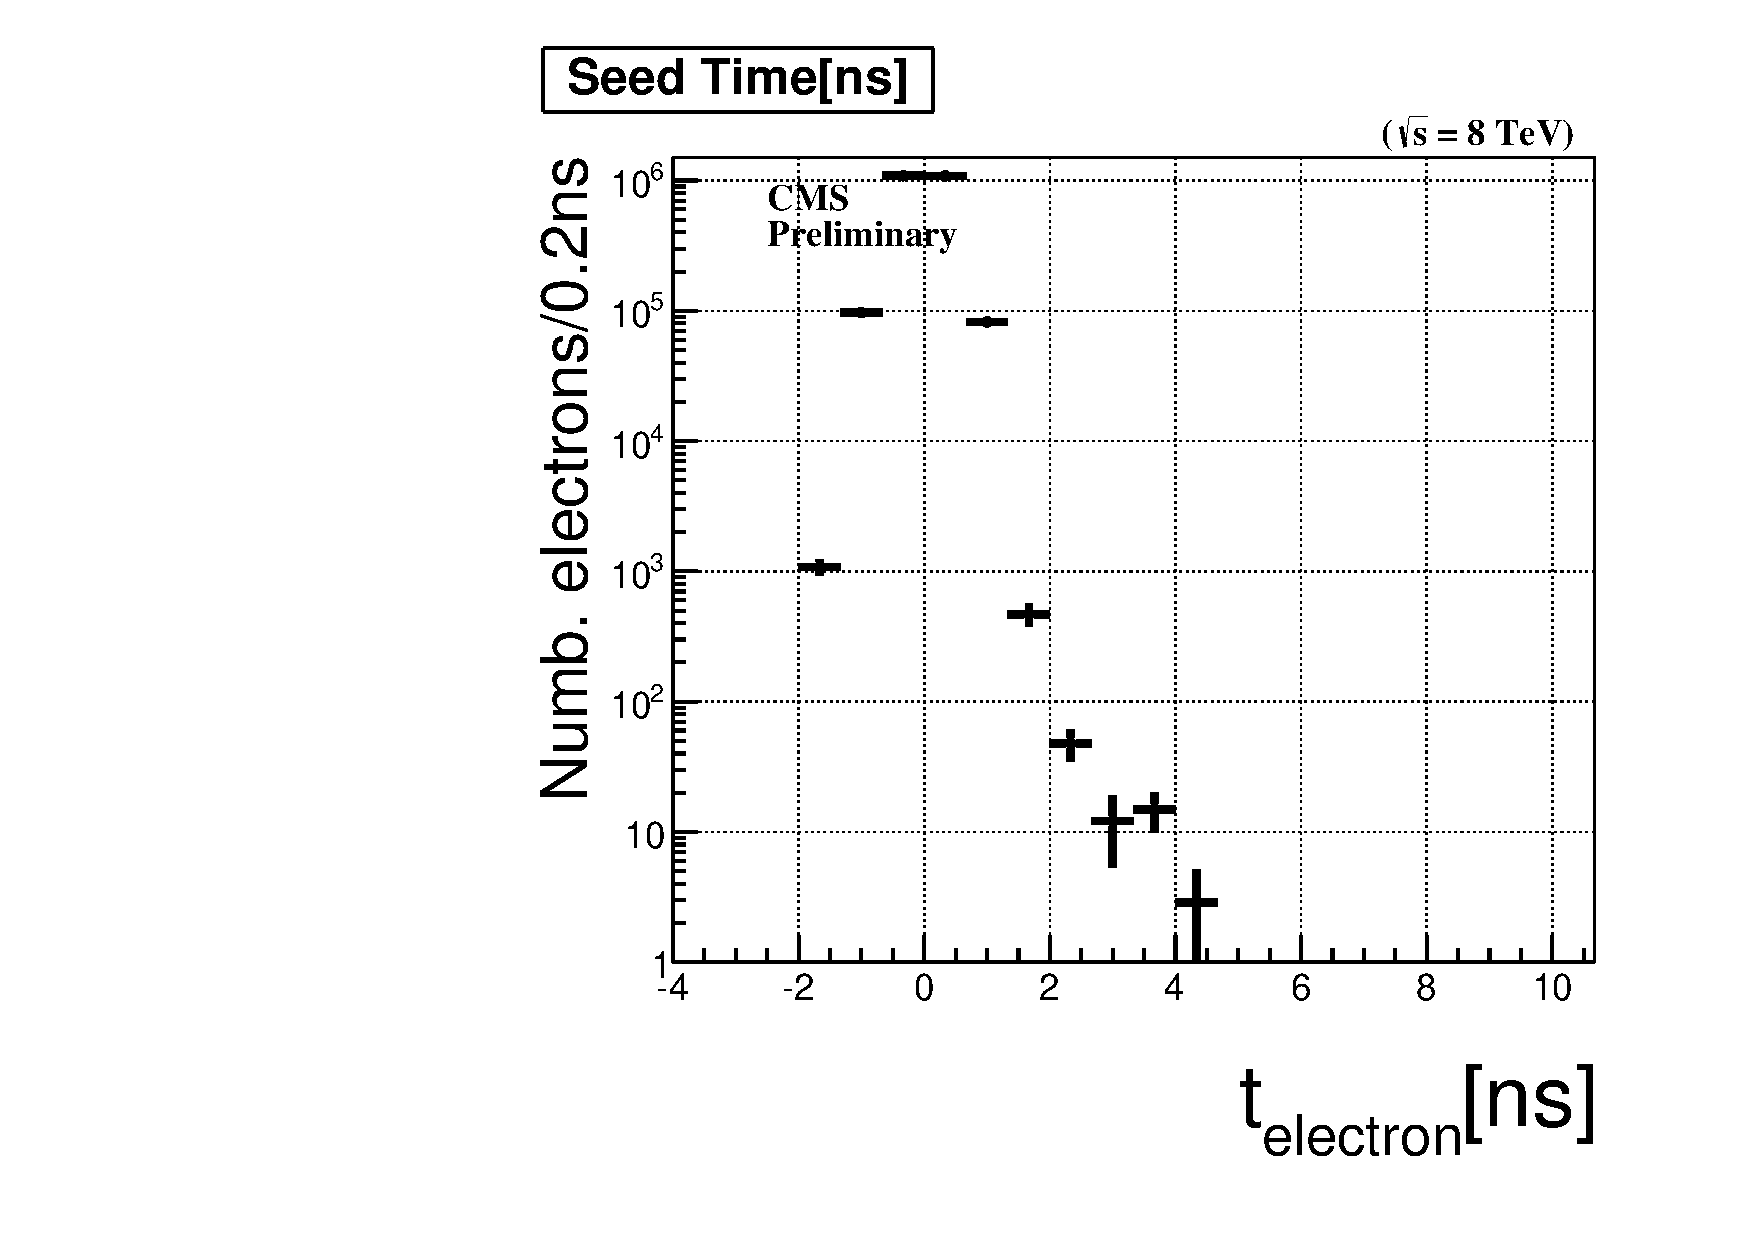
\includegraphics[height=0.55\textwidth, width=0.7\textwidth]{THESISPLOTS/Seed-Time-From-Uncleaned-di-photon-Mass-Fit-DoubleElectron-Run2012A.pdf}
%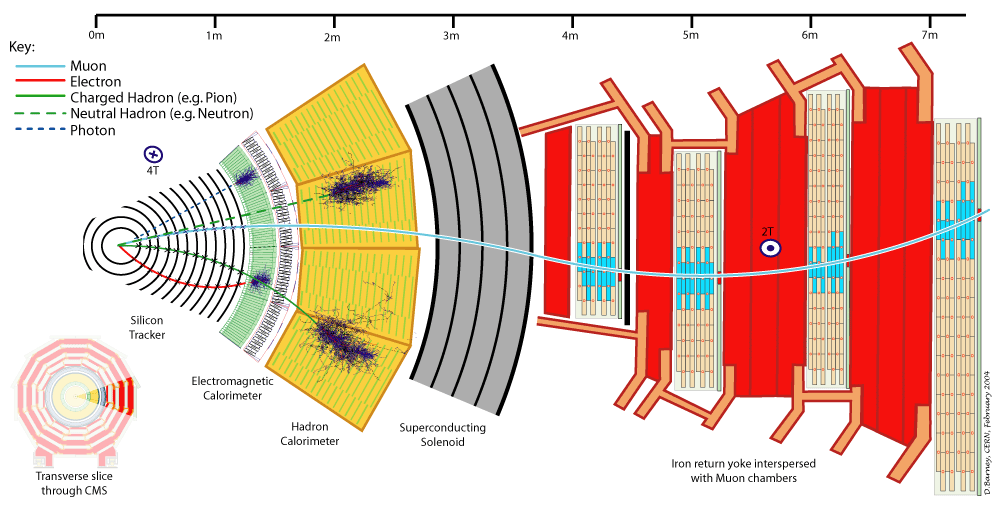
\includegraphics[scale=0.2]{THESISPLOTS/CMS_Slice.png}
%%\captionof{figure}{ECAL time distribution of genuine $\PZ$ bosons after background contribution is subtracted.}
%%\label{fig:Ztime}
%%\end{center}
%%\end{minipage}

\section{Results}
After running our analysis on the SinglePhoton data samples requiring events with at least 2 jets, at least one photon with ECAL time  $ 3.0 < t_{\gamma} < 13.0$\ns, ${\ETslash}^{\gamma}\hspace{0.25cm} > 60$\GeV, and $\ETslash\hspace{0.25cm} > 60$\GeV, we observe a single event passing all our event selection requirements as a signal candidate. This event has one photon and two jets. The photon has a transverse momentum  of 224\GeVc and an ECAL time of 12.17\ns.
\newline
Our expected number of background events estimated is $0.093^{+0.301}_{-0.047}$ which was computed as
\begin{align*} 
 N_{D}^{Total} &= \left( \frac{1 - 0.14}{3}\times 0\right) +  0.093 = 0.093^{+0.301}_{-0.047}
\end{align*}
using the event yields presented in Table \ref{tab:EVTYIELD}.
%% N_{B}^{col} &= \frac{28246}{604958} \times 3 = 0.140^{+0.108}_{-0.061} \\
%% N_{D}^{col} &= \frac{28246}{604958} \times 2 = 0.093^{+0.093}_{-0.047} \\

\par 
For the final result we use the $\PZ\rightarrow\EE$ method to estimate the collision background. This is because the di-electron candidates sample provides a good sample where the non-collision background contribution is almost negligible and in terms of kinematics is the most appropriate sample to estimate how often the time of an electromagnetic particle is mis-measured. The estimated number of background events from collision contributing to samples \textsc{B} and \textsc{D} and total number of background events is given as
\begin{align*} 
 N_{B}^{col} &= 0.51^{+0.28}_{-0.27} \\
 N_{D}^{col} &= 0.37^{+0.09}_{-0.07} \\
 N_{D}^{Total} &= \left( \frac{1 - 0.51}{3}\times 0\right) +  0.37 = 0.37^{+0.39}_{-0.07}.
\end{align*}

\par 
Assuming a Poisson distribution for the observed number of events we obtain a upper limit of $4.37$ on the number of signal events at 95\% Confidence Level~(CL) using the one event observed in the signal sample and the estimated $0.37$ background events.

\vspace{5mm}
\begin{minipage}{0.90\linewidth} 
\begin{center}
\begin{tabular}{c|c|c}
\toprule
 \hline
\bfseries{Control Sample} & 0- and 1-jet Events & $\geq 2-$jets Events \\
\hline
\toprule
\textsf{A} & 851 & 3 \\
\textsf{B} & 38 & 1  \\
\textsc{C} & 359 & 0\\
\textsf{D} & 10 & 1 \\
\hline\hline
\bfseries{Collision Background Events} &  \\ \hline \hline
\textsf{A}& 8 &  3\\ 
\textsf{C}& 2 & 1 \\  
\textsf{F} & 35271& 28246 \\    
\textsf{E}&  1445254 & 604958\\             
\hline
\bottomrule
\end{tabular}
\captionof{table}{Number of events used in the validation~(0- and 1-jet events) and final analysis~($\geq2$-jets events) of the \textsf{ABCD} background~(non-collision~(Halo/cosmic/spikes) and collision) estimation. All events must pass photon, jet and \MET selection requirements.}
\label{tab:EVTYIELD} 
\end{center}
\end{minipage}


\begin{comment}
%%\vspace{5mm}
%%\begin{minipage}{0.90\linewidth} 
%%\begin{center}
%%\begin{tabular}{c| c} %| c| c| c }
%%\toprule
%% \hline
%%\bfseries{Control Sample} & \bfseries{Yield }\\%& Beam Halo & Cosmic & Spike \\
%%\hline
%%\toprule
%%\hline \bfseries{Total Events} &  \\ \hline
%%\textsf{D} & 1 \\% 0 & 0 & 0 \\
%%\textsc{C} & 0 \\%& 2 & 1& 0  \\
%%\textsf{B} & 1 \\%& 1&  1 &  1\\
%%\textsf{A} & 3 \\%& 6 & 0 & 0\\
%%\hline \bfseries{Collision Background Events} &  \\ \hline
%%\textsf{A}& 2 \\%& 0 & 0 & 0\\ 
%%\textsf{C}& 4 \\%& 0 & 0 & 0\\  
%%\textsf{F}& 28246 \\%& -& - & -\\    
%%\textsf{E}& 604958 \\%& - & - & \\       
%%\hline
%%\bottomrule
%%\end{tabular}
%%\captionof{table}{Event yields used in our final background estimation for signal candidate events whose final state consist of at least one photon, at least two jets, . }
%%\label{tab:RESULT} 
%%\end{center}
%%\end{minipage}
%\vspace{5mm} 
\end{comment}

\label{Search_Analysis_chapter}

%\paragraph*{}\mbox{}\\
%\begin{minipage}{\linewidth} 
%\begin{center}
%\centering
%%\begin{tabular}{|c| c| c|}
%%%\mbox{Fake Rate }
%%\toprule
%%\hline
%%\bfseries{Non-Collision} & $\mathbf{{\ETslash}^{\gamma}\hspace{0.15cm}} < 60$\GeV & $\mathbf{{\ETslash}^{\gamma}\hspace{0.15cm}} > 60$\GeV \\
%%\hline
%% $3.0 < t_{\gamma} < 13.0$~ns & \textsf{$C$}($0$) & ~\textsf{$D$}(\textcolor{blue}{$1$}) \\
%% $-10.0 < t_{\gamma} < -3.0$~ns & \textsf{$A$}($5$) & ~\textsf{$B$}($1$) \\
%%\hline \hline
%%\bfseries{Collision} & $\mathbf{\ETslash\hspace{0.15cm}} < 60$\GeV & $\mathbf{\ETslash\hspace{0.15cm}} > 60$\GeV \\
%%\hline 
%% $3.0 < t_{\gamma} < 13.0$~ns & \textsf{$D$}($5$) & ~\textsf{D} \textcolor{red}{$0.0888 ^{+0.1869}_{-0.0444}$} \\
%% $-2.0 < t_{\gamma} < 2.0$~ns & \textsf{$F^{\prime}$}($657663$) & ~\textsf{$F$}($30242$) \\
%% $-10.0 < t_{\gamma} < -3.0$~ns & \textsf{$B$}($1$) & ~\textsf{$B$} $0.23 ^{+0.092}_{-0.118}$) \\
%%\hline
%%\bottomrule
%%\end{tabular}
%%\captionof{table}{Result of observed events and estimated background from signal sample, events with at least $2$-jets. Numbers in bracket represent our observed number of events while numbers not is bracket are our expected number of background events estimated using \textsf{ABCD} method.}
%%\label{tab:RF} 
%%\end{center}
%%\end{minipage}
%%\paragraph*{}\mbox{}\\

%% ECAL Timing
%Algorithms for extracting and calibrating ECAL crystals using the reconstructed hit~(\textit{rechit}) time have been developed
%and we describe them in detail in the coming sections.
%We use $t_{reco}$ to denote the reconstructed time of each hit or crystal.
%We will denote the calibrated reconstructed time of an electromagnetic object as, $T_{reco}$. 
%Measuring the difference of the ECAL measured time between any two reconstructed objects~(which can be individual crystals or electromagnetic objects) arriving from the same nominal point, which in principle are both expected to have the same time, gives a reliable measurement of the timing resolution of the sub-detector including the crystal-to-crystal synchronization factor.  In ECAL timing, the photon reconstructed time, $t_{reco}$, can be calculated using either of the following methods:
%%\begin{enumerate}
%%\item \textbf{seed time}: The time of the highest energy crystal or hit in the highest energy basic cluster~(about $9$ crystals) of the photon super cluster~(about $25$ crystals). It is denoted 
%%\item \textbf{Average or mean time}: This is the error weighted average time of all the crystals in the photon seed basic cluster.
%%It is denoted as $t_{Ave}$ or $t_{mean}$.
%%\end{enumerate}
%Therefore, the arrival time of a photon or an electromagnetic object, $t_{\gamma}$ or $t_{\Pepm}$, can either be given as $t_{seed}$ or $t_{Ave}$.


%%% Useless intro
%\par 
%Non-collision events with photons from cosmic, \textit{beam halo} muons and \textit{spikes} can also have large ECAL time measurements. $pp$ collision events with \PW, \PZ, multiple jets and $\gamma +$jet(s) where the electron or jet is misidentified as a photon and its arrival time mismeasured, can also give rise to large ECAL time photons. And if these events happen to have \MET due to finite detector resolution(\ie instrumental \MET), it is possible for them to be misidentified as the decay of a long-lived neutral particle. We refer to these kinds of events as background events.
%\par 
%To estimate the background contamination to signal, we  use a data driven approach where we divide our data sample using ECAL time, jet multiplicity and \MET into different control samples~(CRs). After rejecting events with spikes, cosmic and beam halo muons, we employ an \textsf{ABCD} background estimation method to estimate background events contributing to the signal sample. 
%\newline 
%Our analysis approach is to count the number events with late photon(s) from proton-proton collision we observed compared to the number of background events we expected.
%Events containing \textit{spikes} produced when particles like high \pt neutrons by-pass the $\pb$ crystals and hit directly the photo-detectors~(APDs) is also a source of isolated early and also late arrival photons. Although  ECAL time measurements of most spikes show they are isolated and have high \pt, with arrival time much earlier compared to "\textit{normal}" photons produced at the nominal proton-proton interaction region whose calibrated average arrival time at ECAL is 0~ns. These different sources of background make it challenging to distinguish a possible signal photon from these separate background photons.
%\newline 
%Together with photons produced from non-collision, events from $pp$ collisions with misreconstucted ECAL time can equally contribute to the tails of the photon time distribution.
% can mimic the signal of an isolated late photon, with large \MET and multiple jets. In the case where the \PW decay into and electron and neutrino, the electron or jet is mis-identified as a photon and its ECAL time miss-measured during event reconstruction, while the undetected photon is identified as \MET. Events where the \PZ boson decays into neutrinos, have large \MET and if the associated jet(s) is mis-identified as photons and their ECAL time mis-measured, such events could mimic signal events with late photons.
%We expect a typical signal event of the decay of a massive neutral long-lived particle, to be produce in a  proton-proton~($pp$) collision at the LHC and detected with the CMS detector, according to the prediction of a benchmark Gauge Mediating Supersymmetry Breaking~(GMSB) model described as the "Snowmass Points and Slope 8"~(SPS8). In this model, the massive long-lived neutral particle is the Next-to-Lightest Supersymmetric Particle~(NLSP) which is the lightest neutralino~(\PSneutralinoOne).

%It decay into a photon~(\Pphoton) and the,  $\PSneutralinoOne\rightarrow\Pphoton + \tilde{G}$. The $ \tilde{G}$  is undetected because it does not interacts with the CMS detector material and as a result, its presence is indirectly inferred by measuring the missing transverse momentum~(\MET). The photon, because of the long-lived nature of the \PSneutralinoOne, arrives late at the ECAL compared to photons produced from nominal $pp$ collisions. 
%\par
%The \PSneutralinoOne can be produced, at the LHC, alone~($\Pquark\APquark\rightarrow \PSgxpm\PSneutralinoOne$) or as a pair~( $\Pquark\APquark\rightarrow \PSneutralinoOne\PSneutralinoOne$), through the direct interaction of the quarks/gluons~(partons) inside the proton. In our analysis, we are interested in the indirect production of the \PSneutralinoOne from  This is because the gluino/squark production cross-section is relatively large at a $pp$ collider like the LHC, since it is a strong interaction process. 
%in association with the \PSneutralinoOne decay, these signal events also contain  and this provide an  requirement useful for suppressing background events without jets.
 %Finding such an event with the CMS detector will be evidence of a new physics phenomena. 
%\par 
%Our signal event must have at least one high-\pt delayed photon, a number of high-\pt jets and large missing transverse momentum(\MET).
%of the neutralino decay, $\PSneutralinoOne \rightarrow \Pphoton + \tilde{G} $, 
%possible new physics parameter space used for the present physics analysis involves: $\tan(\beta) = 15$, $sign(\mu) = 1$, and $\mathbf{M}_{m} = 2\mathbf{\Lambda}$. While $c\tau$ and $\mathbf{\Lambda}$ are used to scan the available parameter space which maximises the sensitivity of the CMS detector to long-lived particles, in this scenario mostly neutralinos~($\tilde{\chi}^{0}_{1}$). The cascade decay of higher mass SUSY particles in the SUSY spectrum to $\tilde{\chi}^{0}_{1}$ allows for signal events with the following constituents:
%\begin{itemize}
%\par
%Our background events could be produce from $pp$ collisions which we call \textit{collision background events} and from non-$pp$ collisions which we call \textit{non-collision background events}, like the so-called beam halo, cosmic muons and spikes. .
%%%%%%%%%%%%%%%%%%%%%%%%%%%%%%%%%%%%%%%%%%%%%%%%%%%%
%%\subsection{Background Modeling}
%%Although our background estimation study is data-driven, however, we also generated a small sample of  $\gamma +$jet(s) events at leading order cross-section. The $\gamma +$jet(s) MC sample is used for studying ECAL time of simulated events. 
%%\newline
%%We did not produced MC samples for background events with \PW, \PZ and $t\bar{t}$ decays because
%%in addition to the fact that their contribution as background events is small, our high-\pt~($\pt > 80$\GeVc) photon requirement will suppress these background events further as most of the electrons from these events which can be misidentified as photons are not high-\pt photons. 
%%\newline
%%We also did not produce MC samples for spikes, cosmic and beam halo muons as simulations of the %%photon ECAL time is not very reliable especially for those events with large photon ECAL time. 
% eventhough these events have \MET and multijets, there are not so many cases in which the photon have a  large ECAL time because a jet was misidentified as a photon and its ECAL time mismeasured. Another reason we did not use MC samples of these events is because simulations of photon/electron ECAL time is not very reliable especially for those events with large photon/electron ECAL time. 
%One of our event selection requirement is high \pt isolated photons, this should reduce contributions from these collision background events by a lot. 